\subsection{Dinámica de los ITQ's con AWGN y banda limitada}

En esta sección exploramos la respuesta de un sistema de medición de entropías en presencia de ruido aditivo y señales filtradas.
Esta inquietud surge como resultado de la implementación detallada en la sección \ref{sec:ImpFPGA}.
El filtrado es inherente al ancho de banda del sistema de medición y las señales a medir siempre están contaminadas con ruido, por lo tanto es necesario caracterizar la respuesta de nuestro sistema de medición ante estos dos procesos.
Este trabajo es complementario al desarrollo de un sistema de medición de entropías implementado en FPGA.

\subsubsection{Filtrado digital}
\label{sec:filtrado}

Ya sea en la elección de un filtro como en cualquier problema de diseño en ingeniería, generalmente no es posible dar una respuesta posible acerca de cual es al mejor solución. Se discute la posibilidad de la implementación de distintos filtros porque no hay un solo método de diseño ni un solo tipo de filtro mejor para todas las circunstancias. La elección del tipo de filtro depende de la importancia de sus ventajas aplicadas a cada problema.

Un filtro ideal es aquel en el que la respuesta en frecuencia es unitaria en el rango de las frecuencias de paso, cero en la banda de rechazo y no posee banda de transición. Dada la inherente periodicidad de la respuesta en frecuencia para tiempo discreto esta tiene la apariencia de un tren rectangular en frecuencias, sin embargo en este trabajo solo se muestra la frecuencia normalizada en el intervalo $(0;1)$. Entonces la transferencia de un pasabajos ideal en frecuencia normalizada quedaría:
\begin{equation}
H_{LP}=
\left\{ 
\begin{aligned}
&1,\qquad|f-0,5|>f_c\\
&0,\qquad|f-0,5|<f_c
\end{aligned}
\right.
\end{equation}
Ecuación definida en el intervalo de frecuencias normalizadas $f\in\left(0,1\right)$.

El hecho de que no podemos contar con series de valores infinitamente largas para ser filtradas, equivale a decir que disponemos de una serie de muestras enventanada.
Como el producto en el dominio del tiempo equivale a una convolución en el dominio de la frecuencia, podemos estudiar el efecto que este enventanado tiene sobre la respuesta frecuencial del filtro.
Consideremos la ventana mas sencilla; la ventana rectangular. Supongamos que la aplicamos sobre una versión retardada de la respuesta ideal, su efecto en el dominio de la frecuencia será la convolución entre la respuesta de nuestro filtro ideal y la transformada esta ventana rectangular, es decir una función $sinc$ de período $1/N$ en donde $N$ es la cantidad de muestras que entran en la ventana.

El efecto de enventanado o truncaminto de la respuesta es doble: por una parte, la anchura del lóbulo principal está relacionada con la aparición de una banda de transición en el filtro. Por otra, la presencia de lóbulos laterales (secundarios) lleva a la aparición de un ripple u oscilaciones en la respuesta en frecuencia, en ambas bandas, (más apreciable en la banda no pasante).
La aparición de los lóbulos secundarios se debe a que la ventana rectangular presenta una discontinuidad abrupta que, al pasar al dominio de la frecuencia, conlleva un reparto de la energía por todo el espectro a causa del aliasing.

Una opción que se plantea es generalizar el concepto de ventana y emplear ventanas más suaves que la rectangular para realizar el truncamiento de la respuesta deseada, esta técnica es una de las formas de realizar un filtro FIR.
Sin embargo, si analizamos la transformada de la ventana cuadrada vemos que presenta valores nulos cada $1/N$, que son los mismos lugares en donde aparecen las componentes espectrales de la DFT. Esto significa que los efectos de la ventana rectangular aparecen al convertir la respuesta de este filtro a tiempo continuo.

Otra opción sería diseñar un filtro analógico y transformar su respuesta a frecuencia discreta. Para esto contamos con fórmulas cerradas de diseño, por lo que podemos satisfacer cualquier especificación preestablecida. La utilización de esta técnica da como resultado un filtro IIR. Comparado con un FIR, un filtro IIR requiere un orden mucho menor para cumplir las especificaciones de diseño.

Aquí analizamos un sistema en el cual la respuesta es analizada en el dominio digital. Además, es necesario filtrar componentes espectrales de a una, lo que requiere una banda de transición muy estrecha, esto reduce el conjunto de filtros posibles. Por el lado del IIR probamos un filro elíptico, este filtro presenta una banda de transición muy estrecha en sacrificio de un ripple que aparece tanto en la banda de paso como en la de rechazo. Por el lado del FIR probamos un filtro ideal con una ventana rectangular que abarca toda la serie de valores, en la sección \ref{sec:resultados} se detalla como fue implementado.

\subsubsection{Resultados}
\label{sec:resultados}

Para representar la dinámica en función del filtrado, se eligieron dos señales representativas (cuadrada y senoidal) y se les calcularon los cuantificadores descriptos en la sección \ref{sec:entropias} luego de ser filtrados por los filtros elegidos en la sección \ref{sec:filtrado}. Por otro lado, se calculan los mismos cuantificadores a una señal de ruido blanco gaussiano.

En la figura \ref{fig:flowchart} se muestra el procedimiento utilizado. Primero se generó un vector de ruido blanco gaussiano de $N=50E3$ muestras, la desviación estándar $\sigma$ es variable y se logra multiplicando al vector inicial de $\sigma=1$ por la desviación estándar elegida.
Luego se genera la señal determinística de $N=50E3$ muestras, período $T=100$ muestras y amplitud unitaria, que se sumó el ruido para lograr la señal contaminada.
La señal resultante se filtra para luego calcular cuantificadores.
Como se explicó más arriba, para calcular le entropía de valores se genera el histograma de valores y se lo normaliza para calcular la Función Densidad de Probabilidad de valores $PDF_{hist}$ a la que se le calcula la entropía de Shannon normalizada que da como resultado la entropía de valores normalizada $H_{hist}$.
Para calcular la entropía de patrones de orden se utiliza el histograma de patrones de orden que cuando se normaliza se consigue la función densidad de probabilidad de patrones de orden $PDF_{BP}$, a la que se le calcula la entropía de Shannon normalizada para conseguir la entropía de patrones de orden $H_{BP}$.
%
\begin{figure}[h]
\centering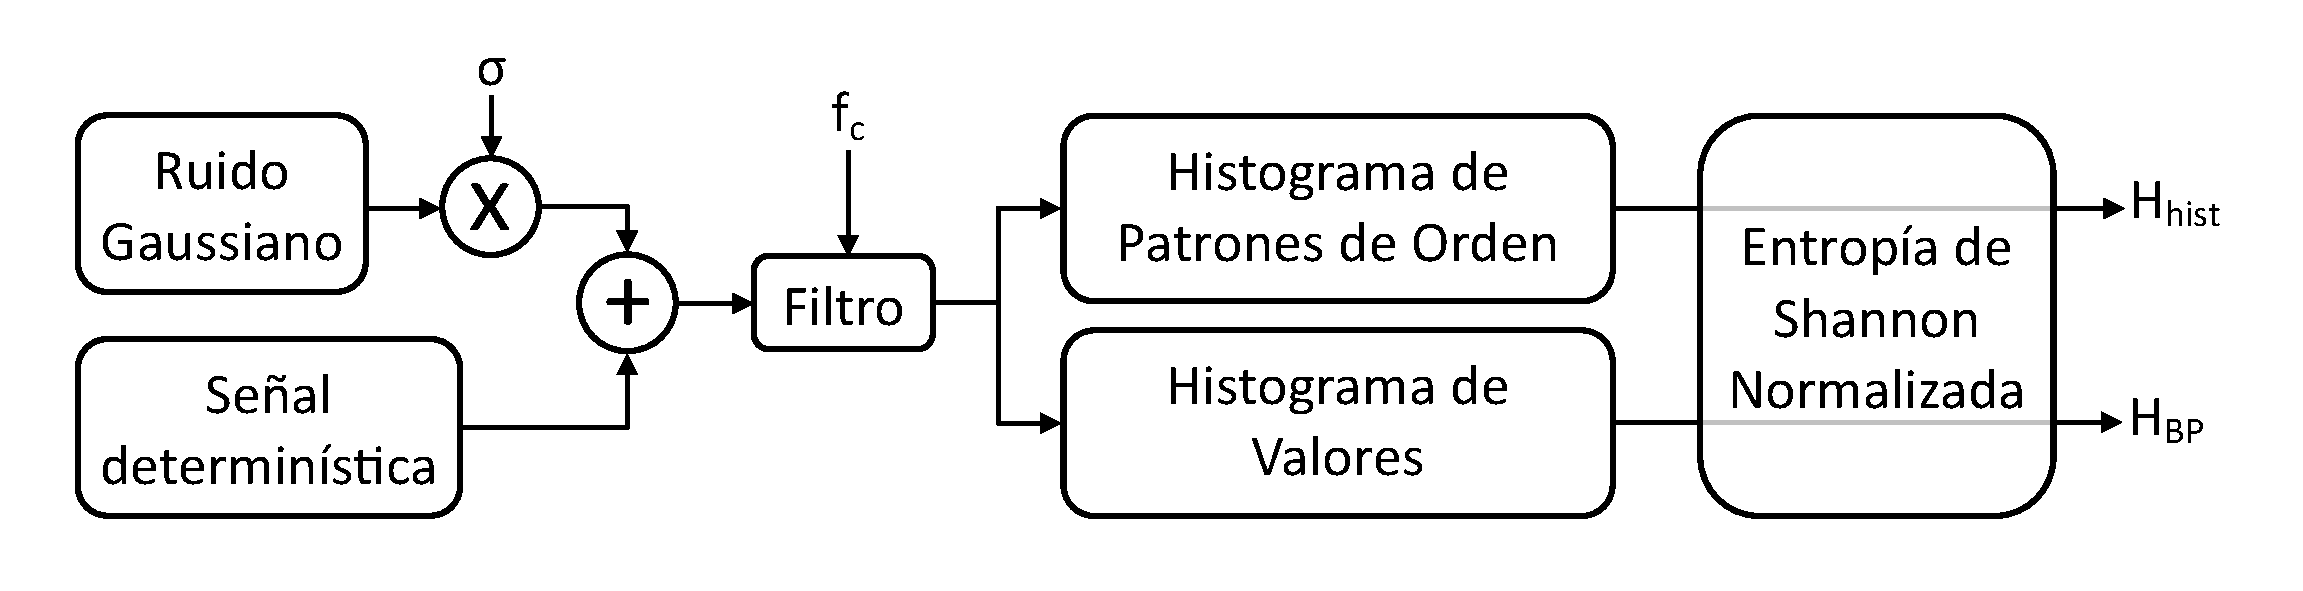
\includegraphics [width=0.99\textwidth]{FlowChart}
\caption {Diagrama de flujo del experimento.}\label{fig:flowchart}
\end{figure}

Para evaluar la contribución de cada componente espectral a las entropías, se evaluaron dos filtros. Primero se aplicó un filtro elíptico de orden $10$ con ripple pasabanda de $0,5 dB$, ripple en la banda de rechazo de $100 dB$ y frecuencia de corte variable $f_c$, en la figura \ref{fig:filtroellip} se muestra su respuesta en ganancia (fig. \ref{subfig:filtroellip_amplitud}) y fase (fig. \ref{subfig:filtroellip_frecuencia}) para el caso de $f_c=0,5$. De esta forma se logra un filtrado lo suficientemente abrupto como para considerar que a medida que se barren distintas frecuencias de corte se eliminan componentes espectrales individualmente.
Los resultados de este filtrado se compararon con los resultados de un filtro ideal (fig. \ref{fig:filtroideal}), que consiste en una máscara aplicada a la transformada de fourier de la señal a filtrar, de esta manera se consigue el espectro de la señal filtrada, el cual es antitransformado para recuperar la versión filtrada en las muestras. El diagrama de este filtro puede verse en la figura \ref{subfig:filtroideal_diagrama}. Este procedimiento equivale a un filtrado ideal sin retardo, por lo que el bode de amplitud es $0dB$ en la banda de paso y $-\infty dB$ en la banda de rechazo (fig. \ref{subfig:filtroideal_diagrama}); la fase $\omega\tau=0$ es lineal con pendiente nula (fig. \ref{subfig:filtroideal_frecuencia}).
%
\begin{figure}[h]
    \centering
    \begin{subfigure}[t]{0.32\textwidth}
        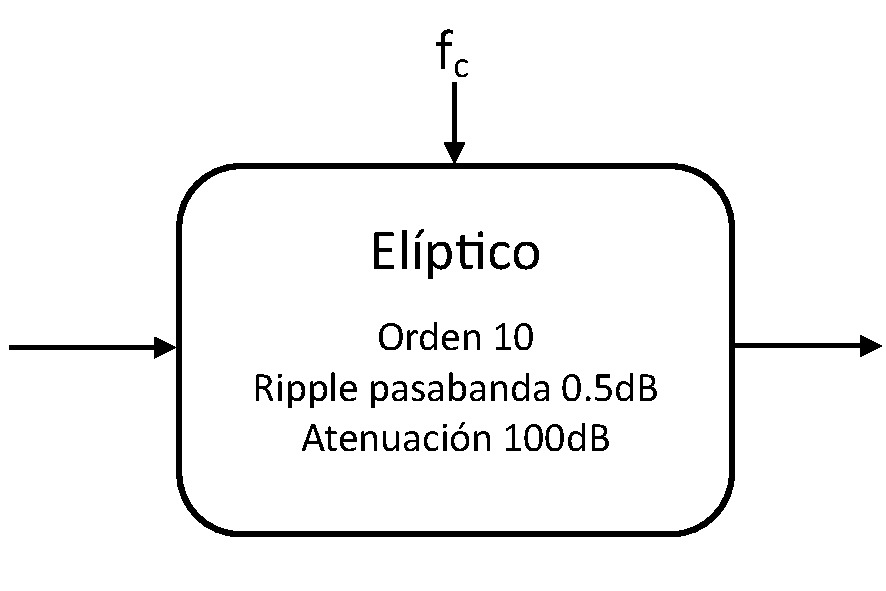
\includegraphics[width=\textwidth]{Ellip}
        \caption{Esquema}
        \label{subfig:filtroellip_diagrama}
    \end{subfigure}
    ~ %add desired spacing between images, e. g. ~, \quad, \qquad, \hfill etc. 
      %(or a blank line to force the subfigure onto a new line)
    \begin{subfigure}[t]{0.32\textwidth}
        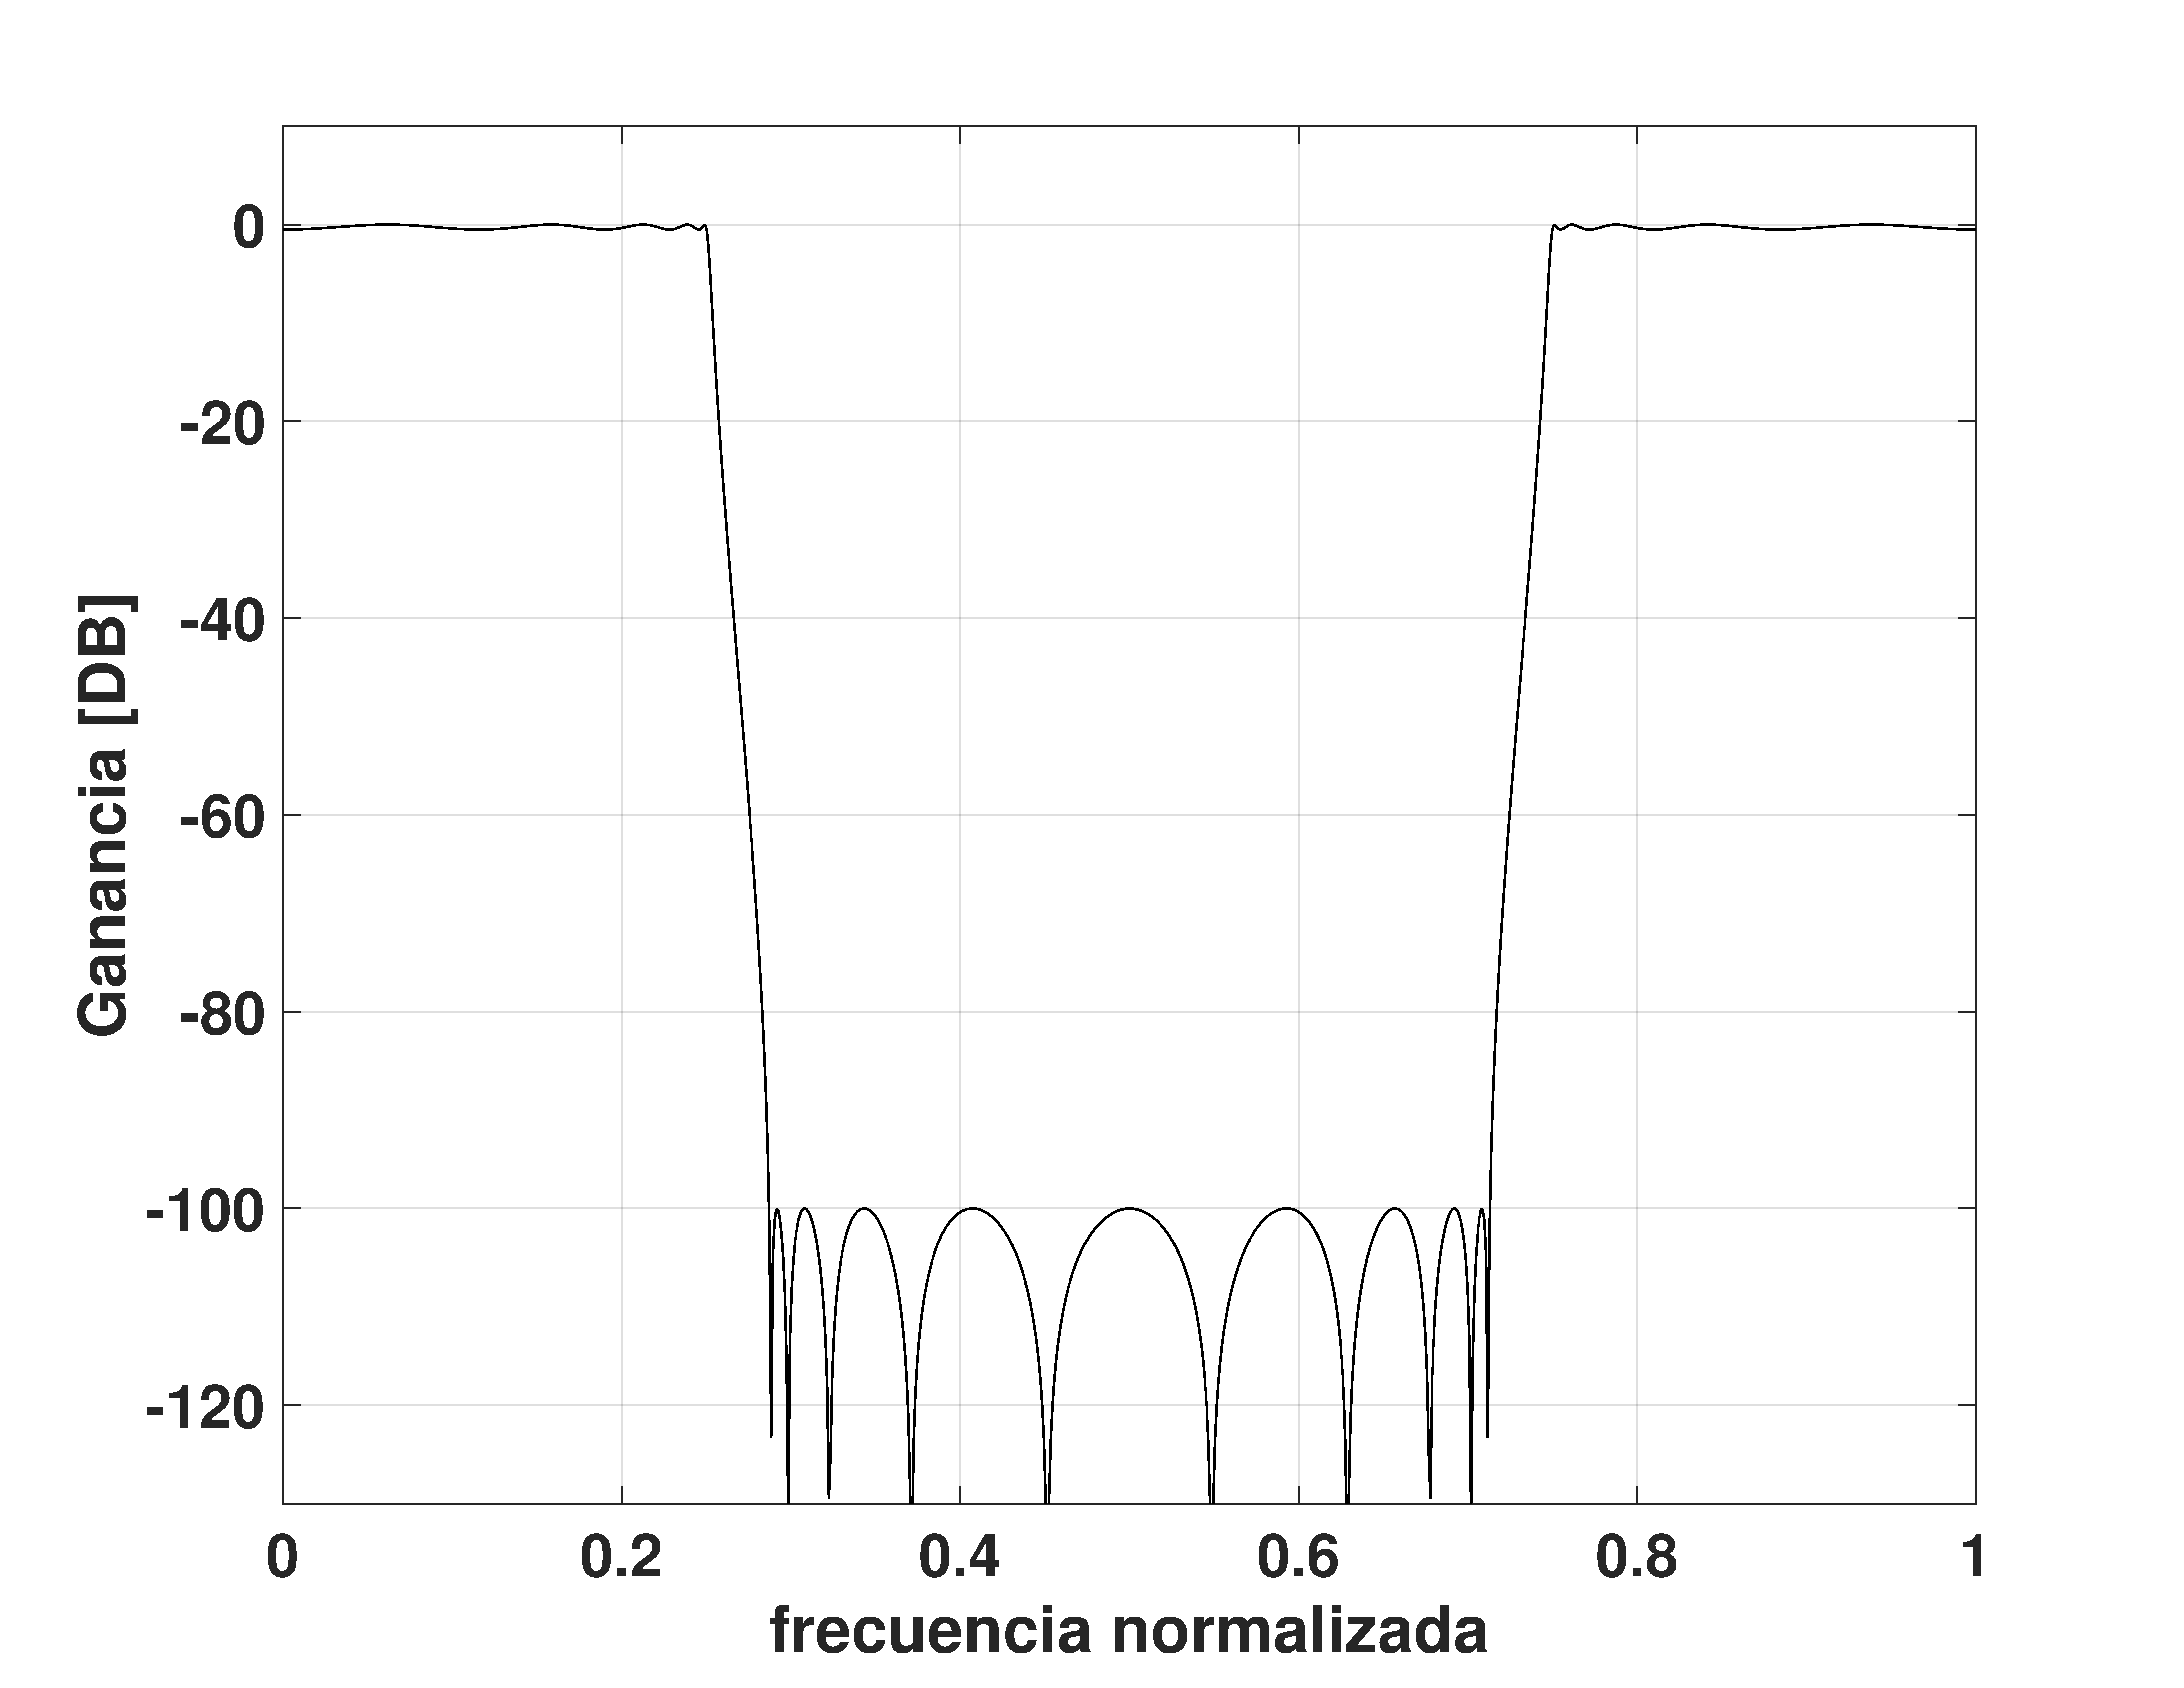
\includegraphics[width=\textwidth]{BodeEllip}
        \caption{Bode de ganancia}
        \label{subfig:filtroellip_amplitud}
    \end{subfigure}
    ~ %add desired spacing between images, e. g. ~, \quad, \qquad, \hfill etc. 
    %(or a blank line to force the subfigure onto a new line)
    \begin{subfigure}[t]{0.32\textwidth}
        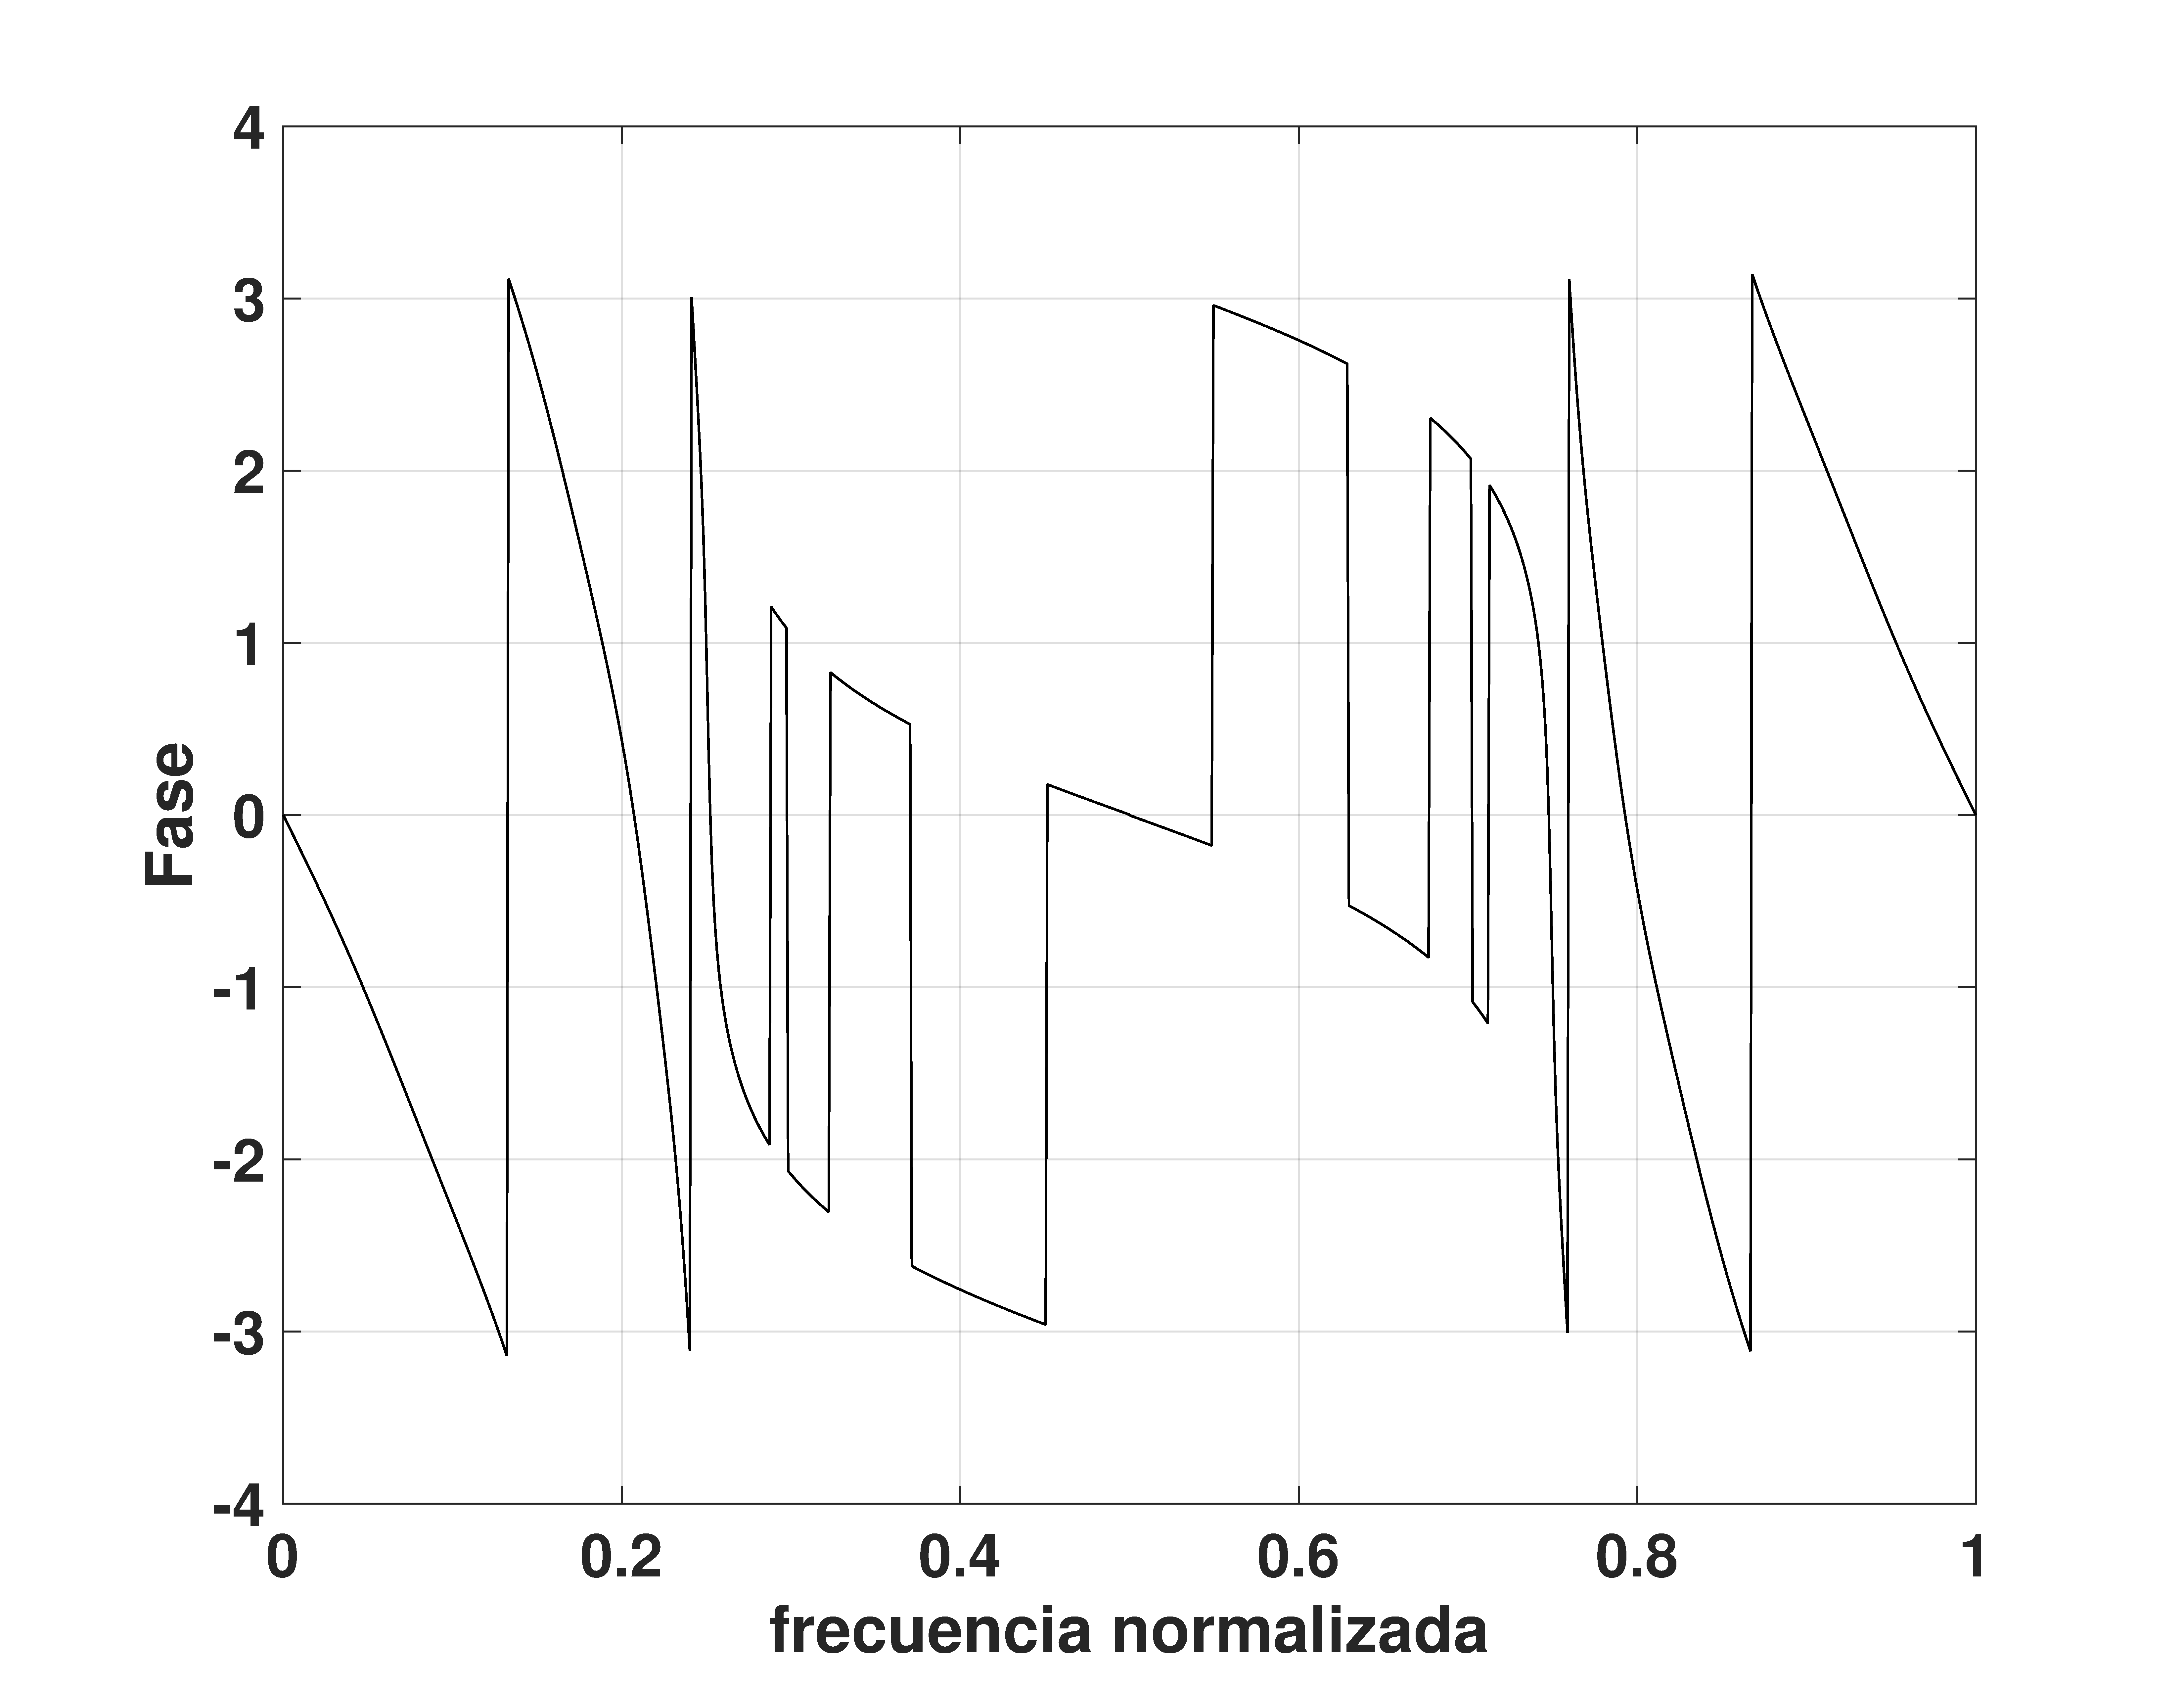
\includegraphics[width=\textwidth]{FreqEllip}
        \caption{Bode de fase}
        \label{subfig:filtroellip_frecuencia}
    \end{subfigure}
    \caption{Filtro elíptico.}\label{fig:filtroellip}
\end{figure}
%
\begin{figure}[h]
    \centering
    \begin{subfigure}[t]{0.32\textwidth}
        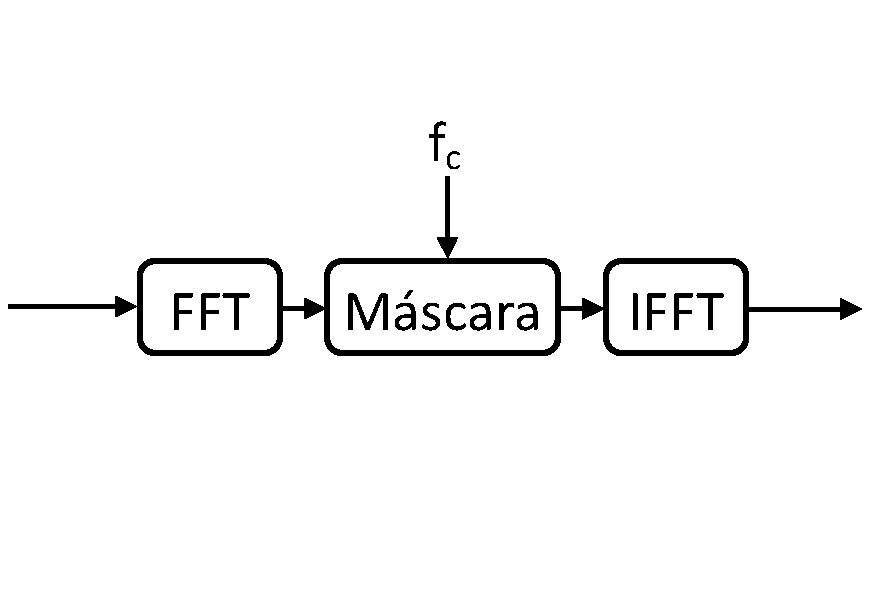
\includegraphics[width=\textwidth]{Ideal}
        \caption{Esquema}
        \label{subfig:filtroideal_diagrama}
    \end{subfigure}
    ~ %add desired spacing between images, e. g. ~, \quad, \qquad, \hfill etc. 
      %(or a blank line to force the subfigure onto a new line)
    \begin{subfigure}[t]{0.32\textwidth}
        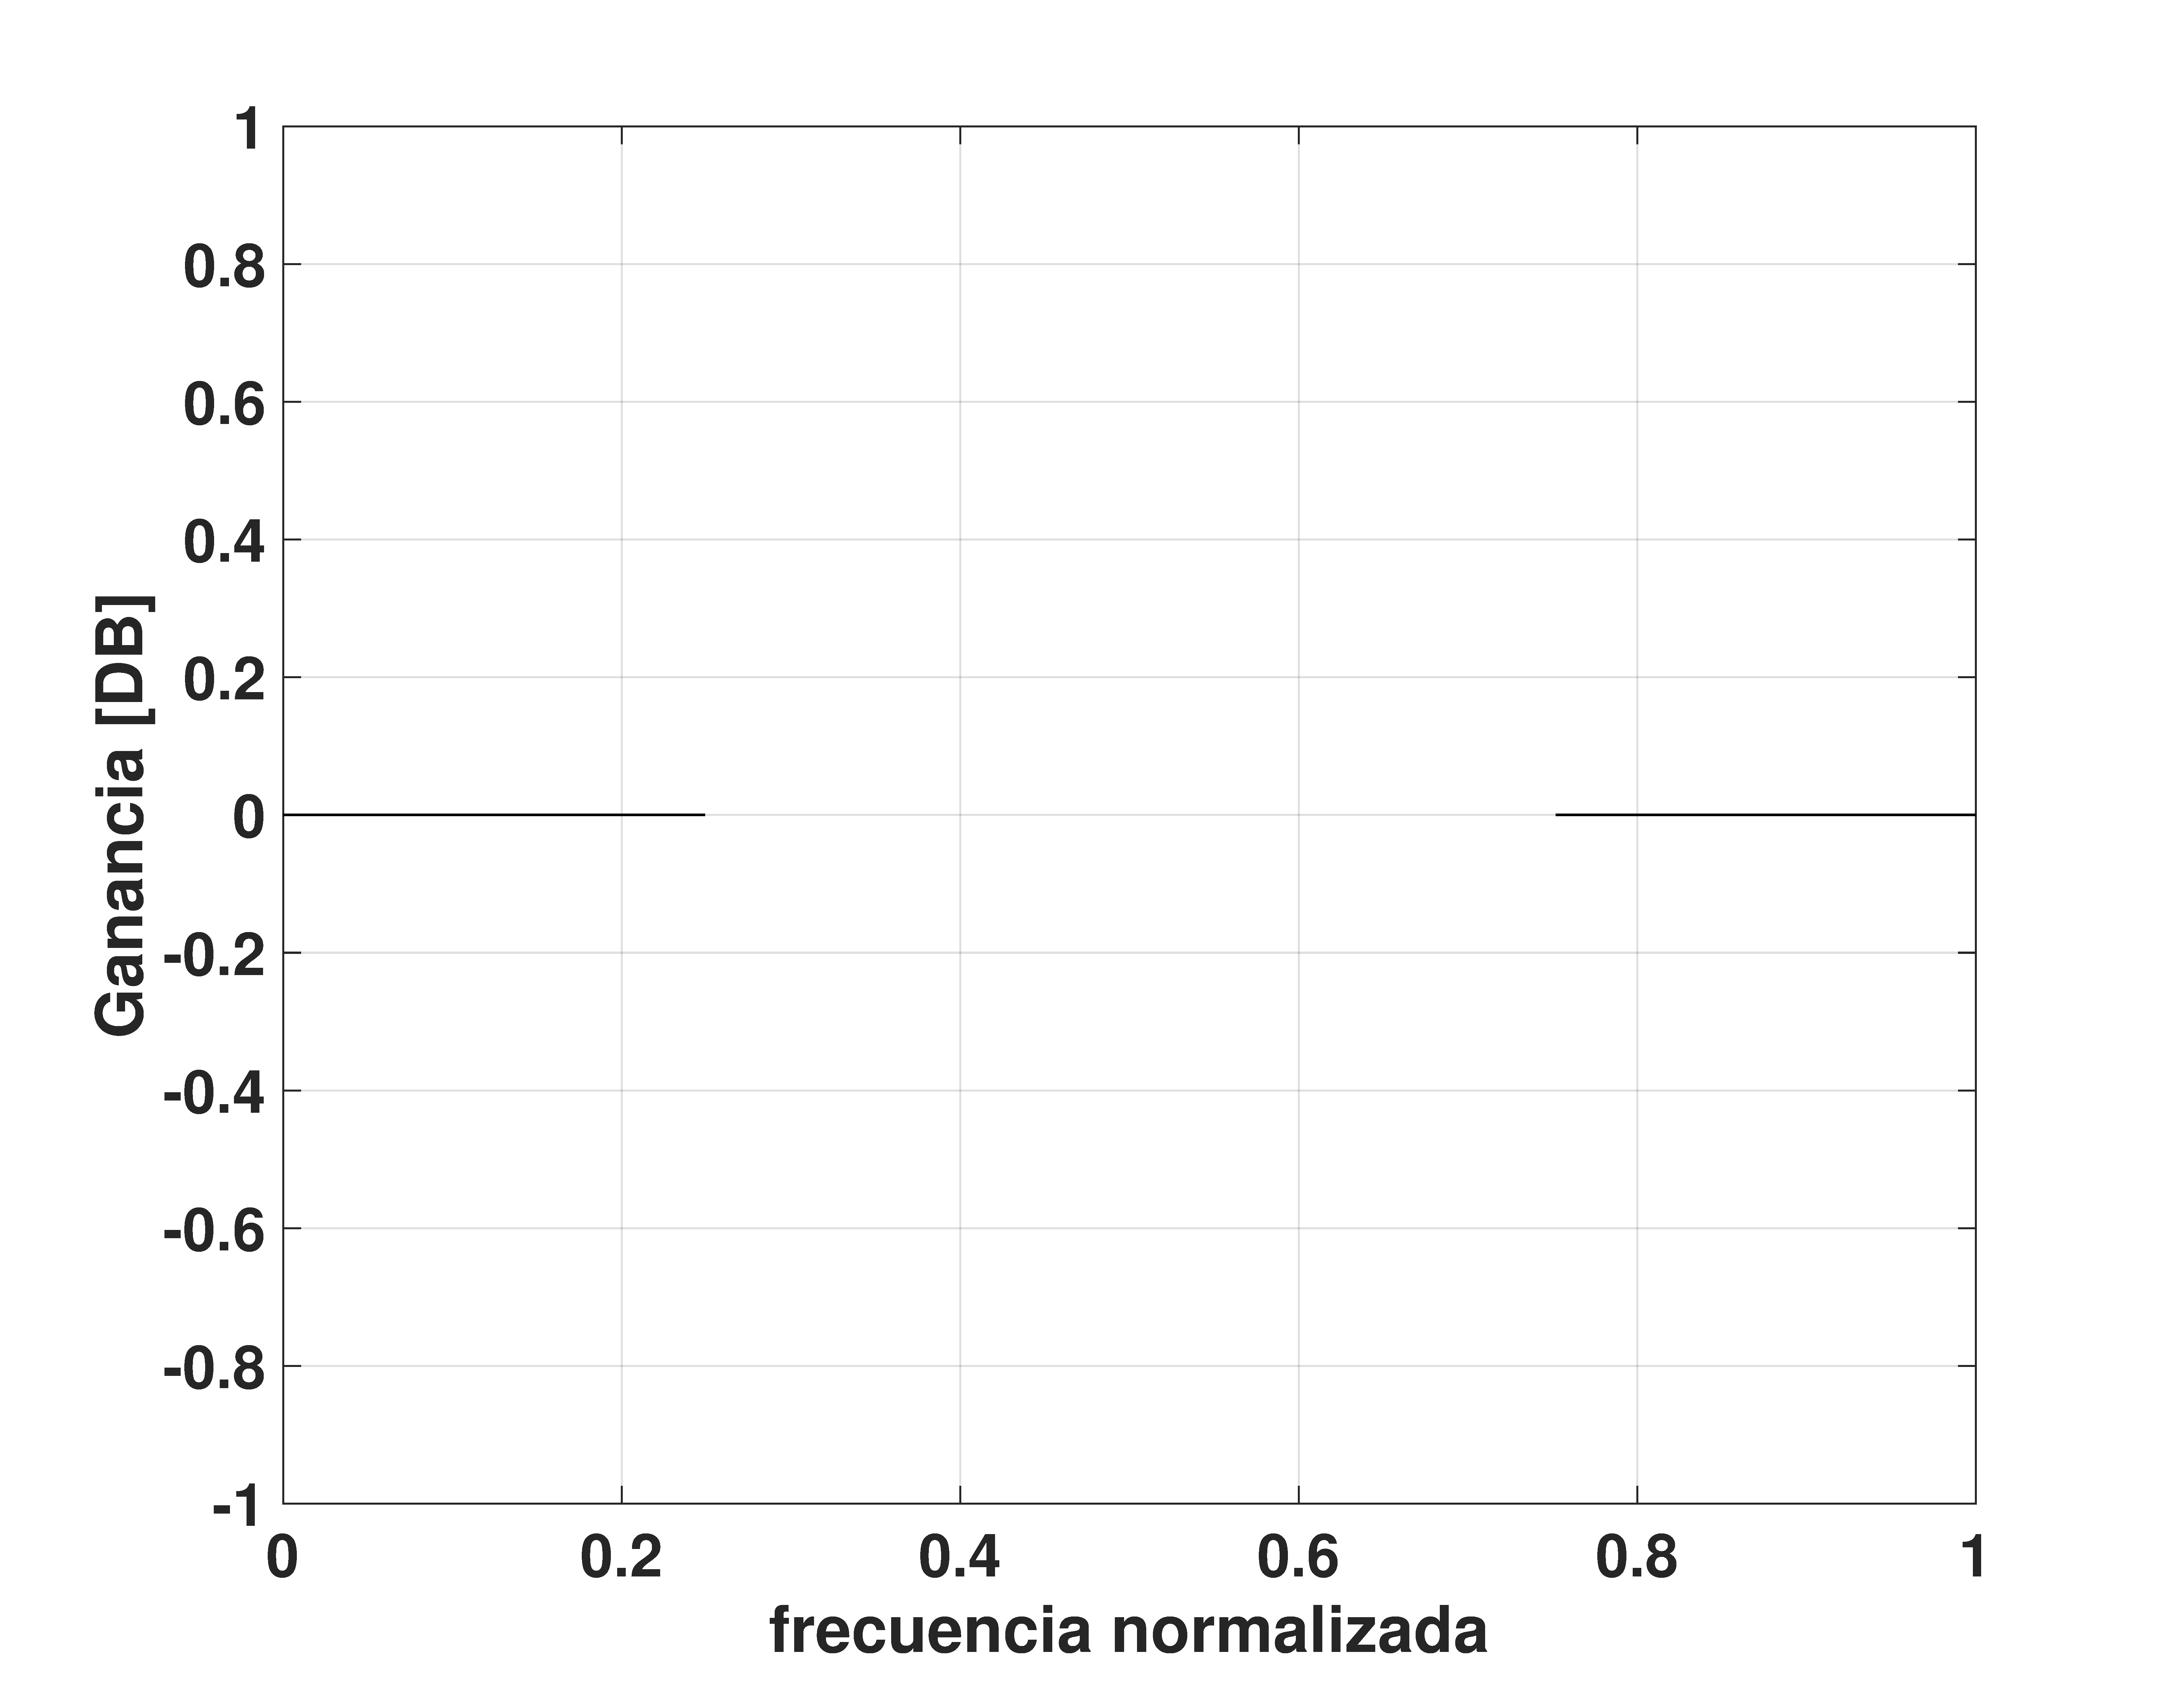
\includegraphics[width=\textwidth]{BodeIdeal}
        \caption{Bode de ganancia}
        \label{subfig:filtroideal_amplitud}
    \end{subfigure}
    ~ %add desired spacing between images, e. g. ~, \quad, \qquad, \hfill etc. 
    %(or a blank line to force the subfigure onto a new line)
    \begin{subfigure}[t]{0.32\textwidth}
        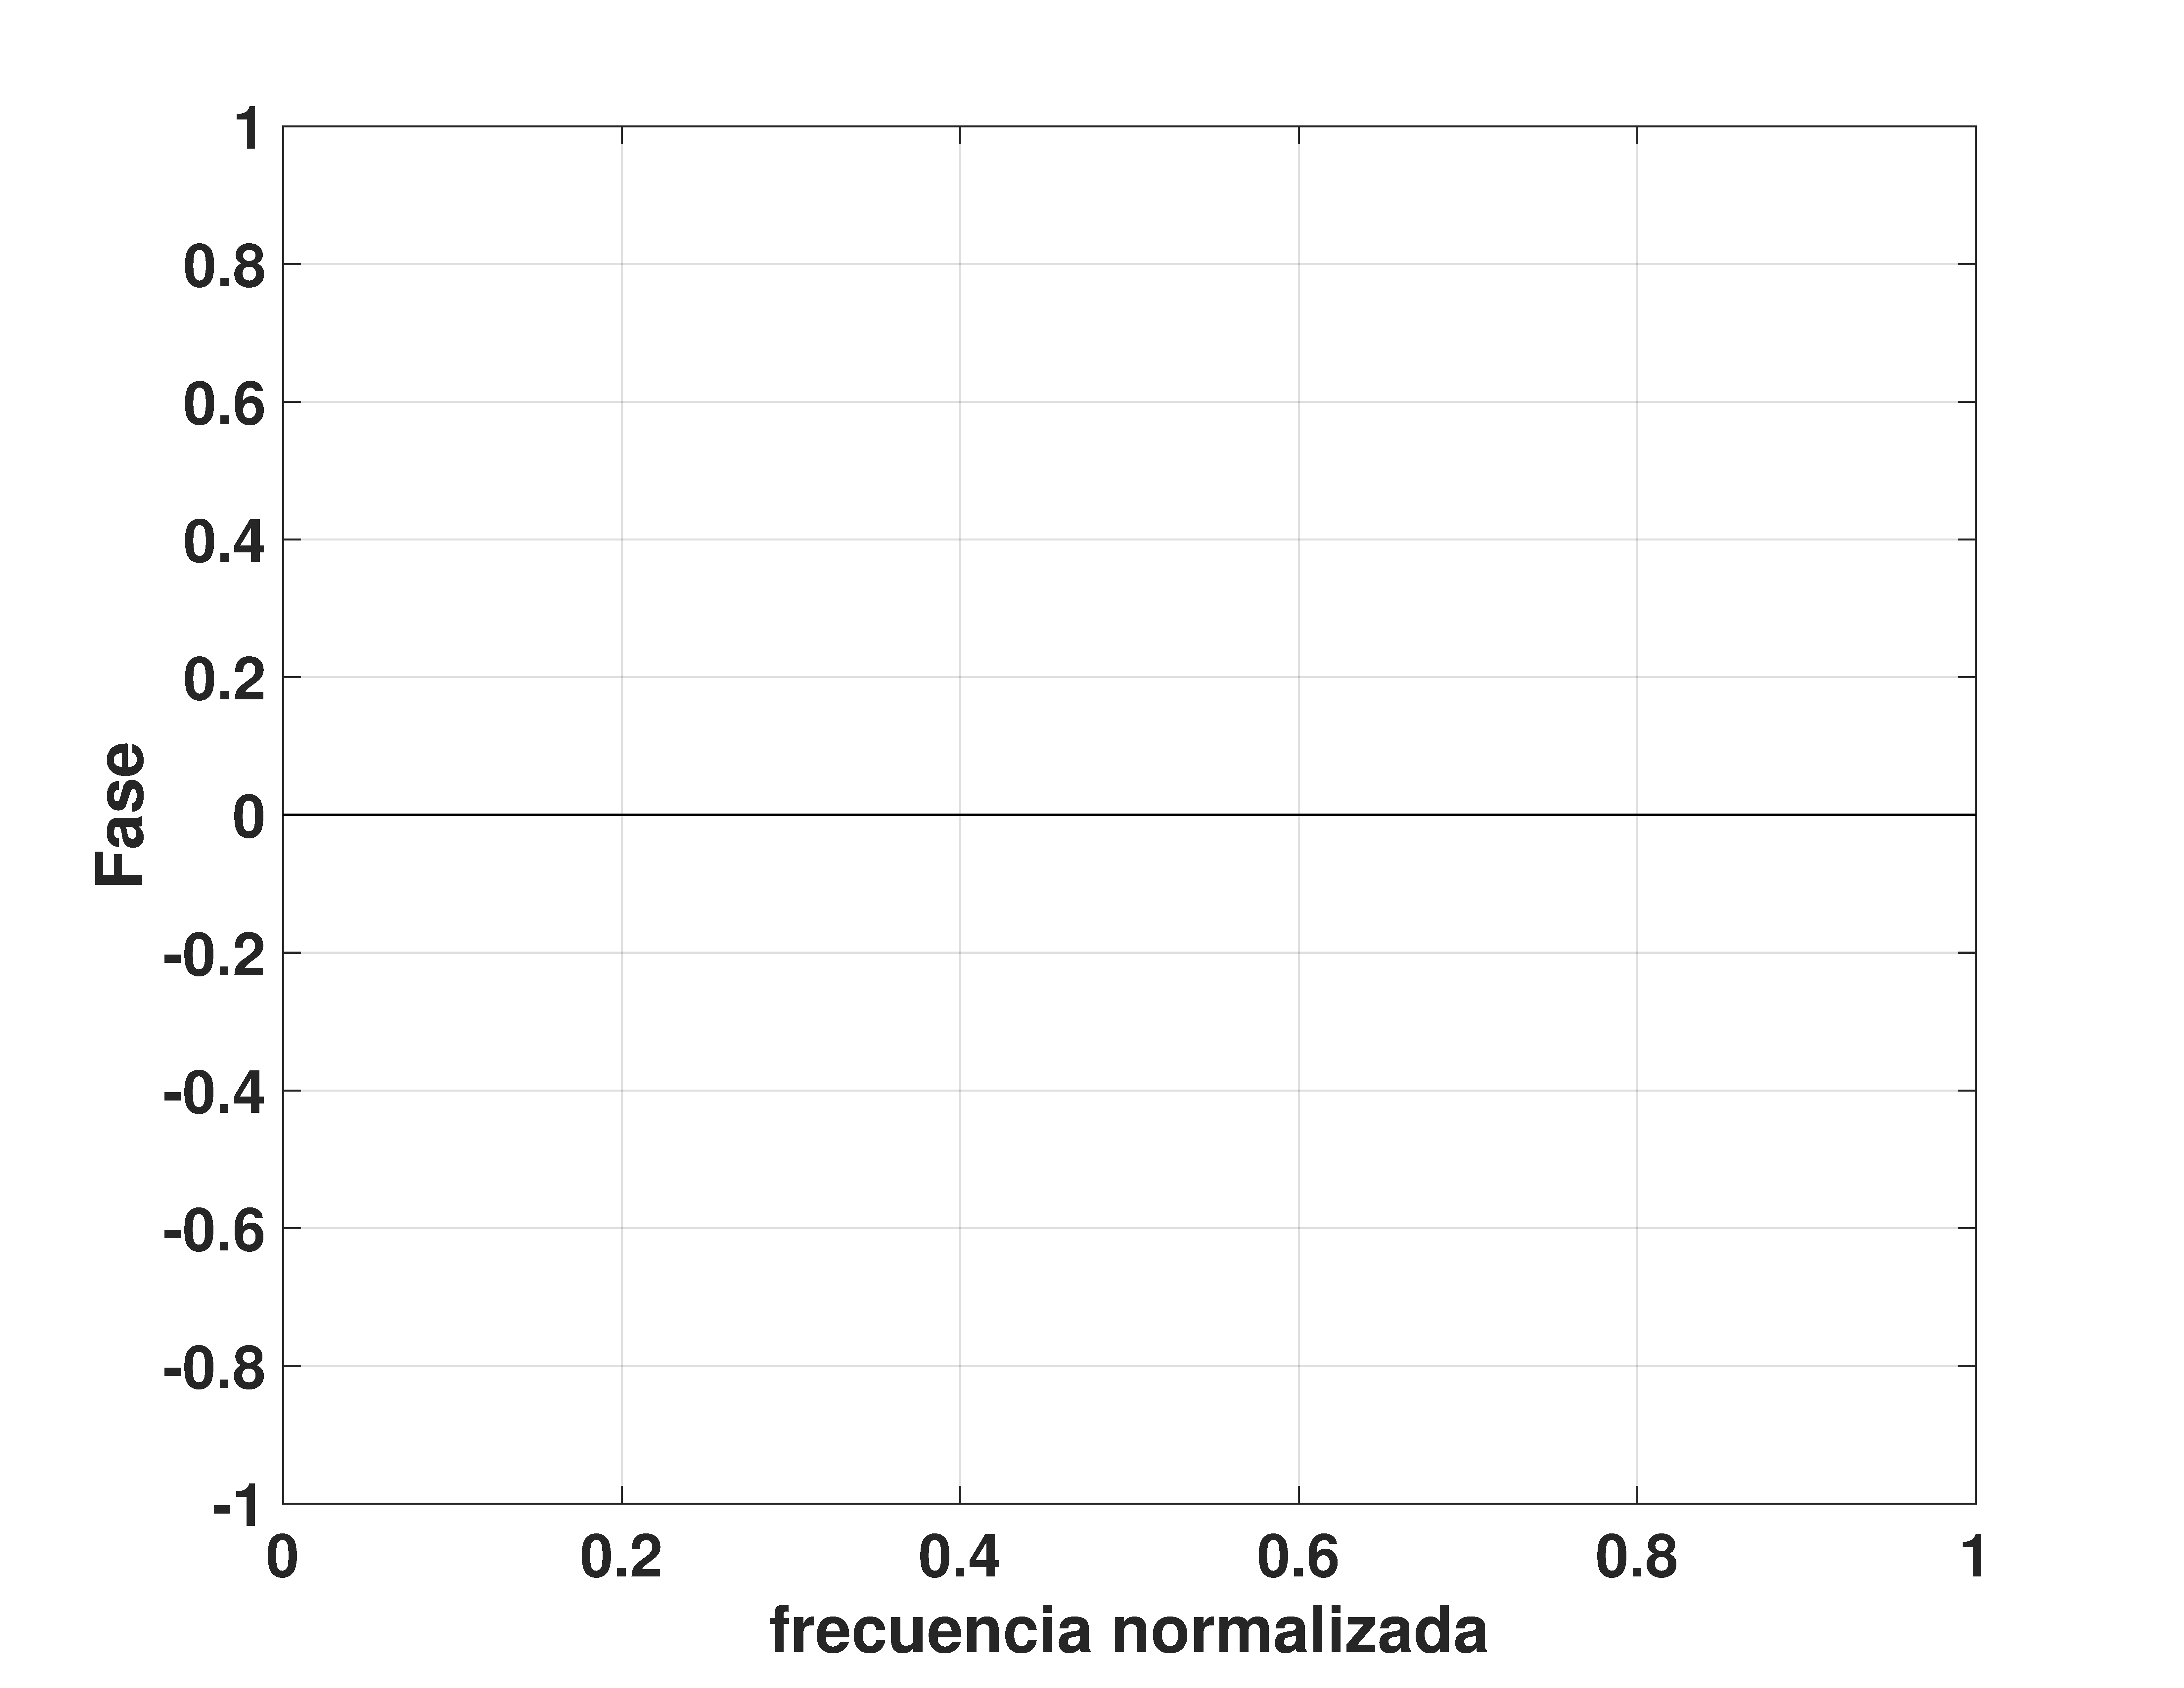
\includegraphics[width=\textwidth]{FreqIdeal}
        \caption{Bode de fase}
        \label{subfig:filtroideal_frecuencia}
    \end{subfigure}
    \caption{Filtro ideal.}\label{fig:filtroideal}
\end{figure}

Primero se aplicó una señal de ruido blanco gaussiano, es decir que la señal determinística es cero y la desviación estándar de la gaussiana unitaria.
En la figura \ref{fig:ellip} se muestra el resultado de los cuantificadores a medida que se va barriendo la frecuencia de corte del filtro elíptico.
En la figura \ref{subfig:ellip_Hhist} se muestra la entropía del histograma de valores $H_{hist}$, puede verse que su valor se mantiene constante alrededor de $0,9$ tanto para el filtro pasa-bajos (roja) como el pasa-altos (azul), este valor es el mismo que resulta de calcular la entropía del histograma de valores a la señal sin filtrar (resultado que se muestra con una línea punteada negra en el mismo plot). También puede verse que cuando la frecuencia de corte del filtro elíptico se acerca a los extremos el valor del cuantificador cae, en estas frecuencias el método numérico que calcula el vector filtrado diverge debido a la precisión finita.
En la figura \ref{subfig:ellip_Hbp} se muestra la entropía de los patrones de orden, $H_{BP}$ se mantiene en valores bajos cuando el filtro (pasa-altos en azul y pasa-bajos en rojo) deja pasar pocas componentes espectrales. Luego, a medida que la frecuencia de corte deja pasar más componentes espectrales, el cuantificador tiende a $1$, que es justamente el valor que arroja cuando se ingresa con la señal sin filtrar (este valor se marca con una línea punteada negra).
El cuantificador detecta los cambios en la forma de la señal a medida que es filtrada.
Por último, en el plano $H_{hist} - H_{BP}$ de la figura \ref{subfig:ellip_HbpHhist} se compacta la información de ambos cuantificadores, aunque se pierde la noción de la frecuencia de corte.
%
\begin{figure}[h]
    \centering
    \begin{subfigure}[t]{0.32\textwidth}
        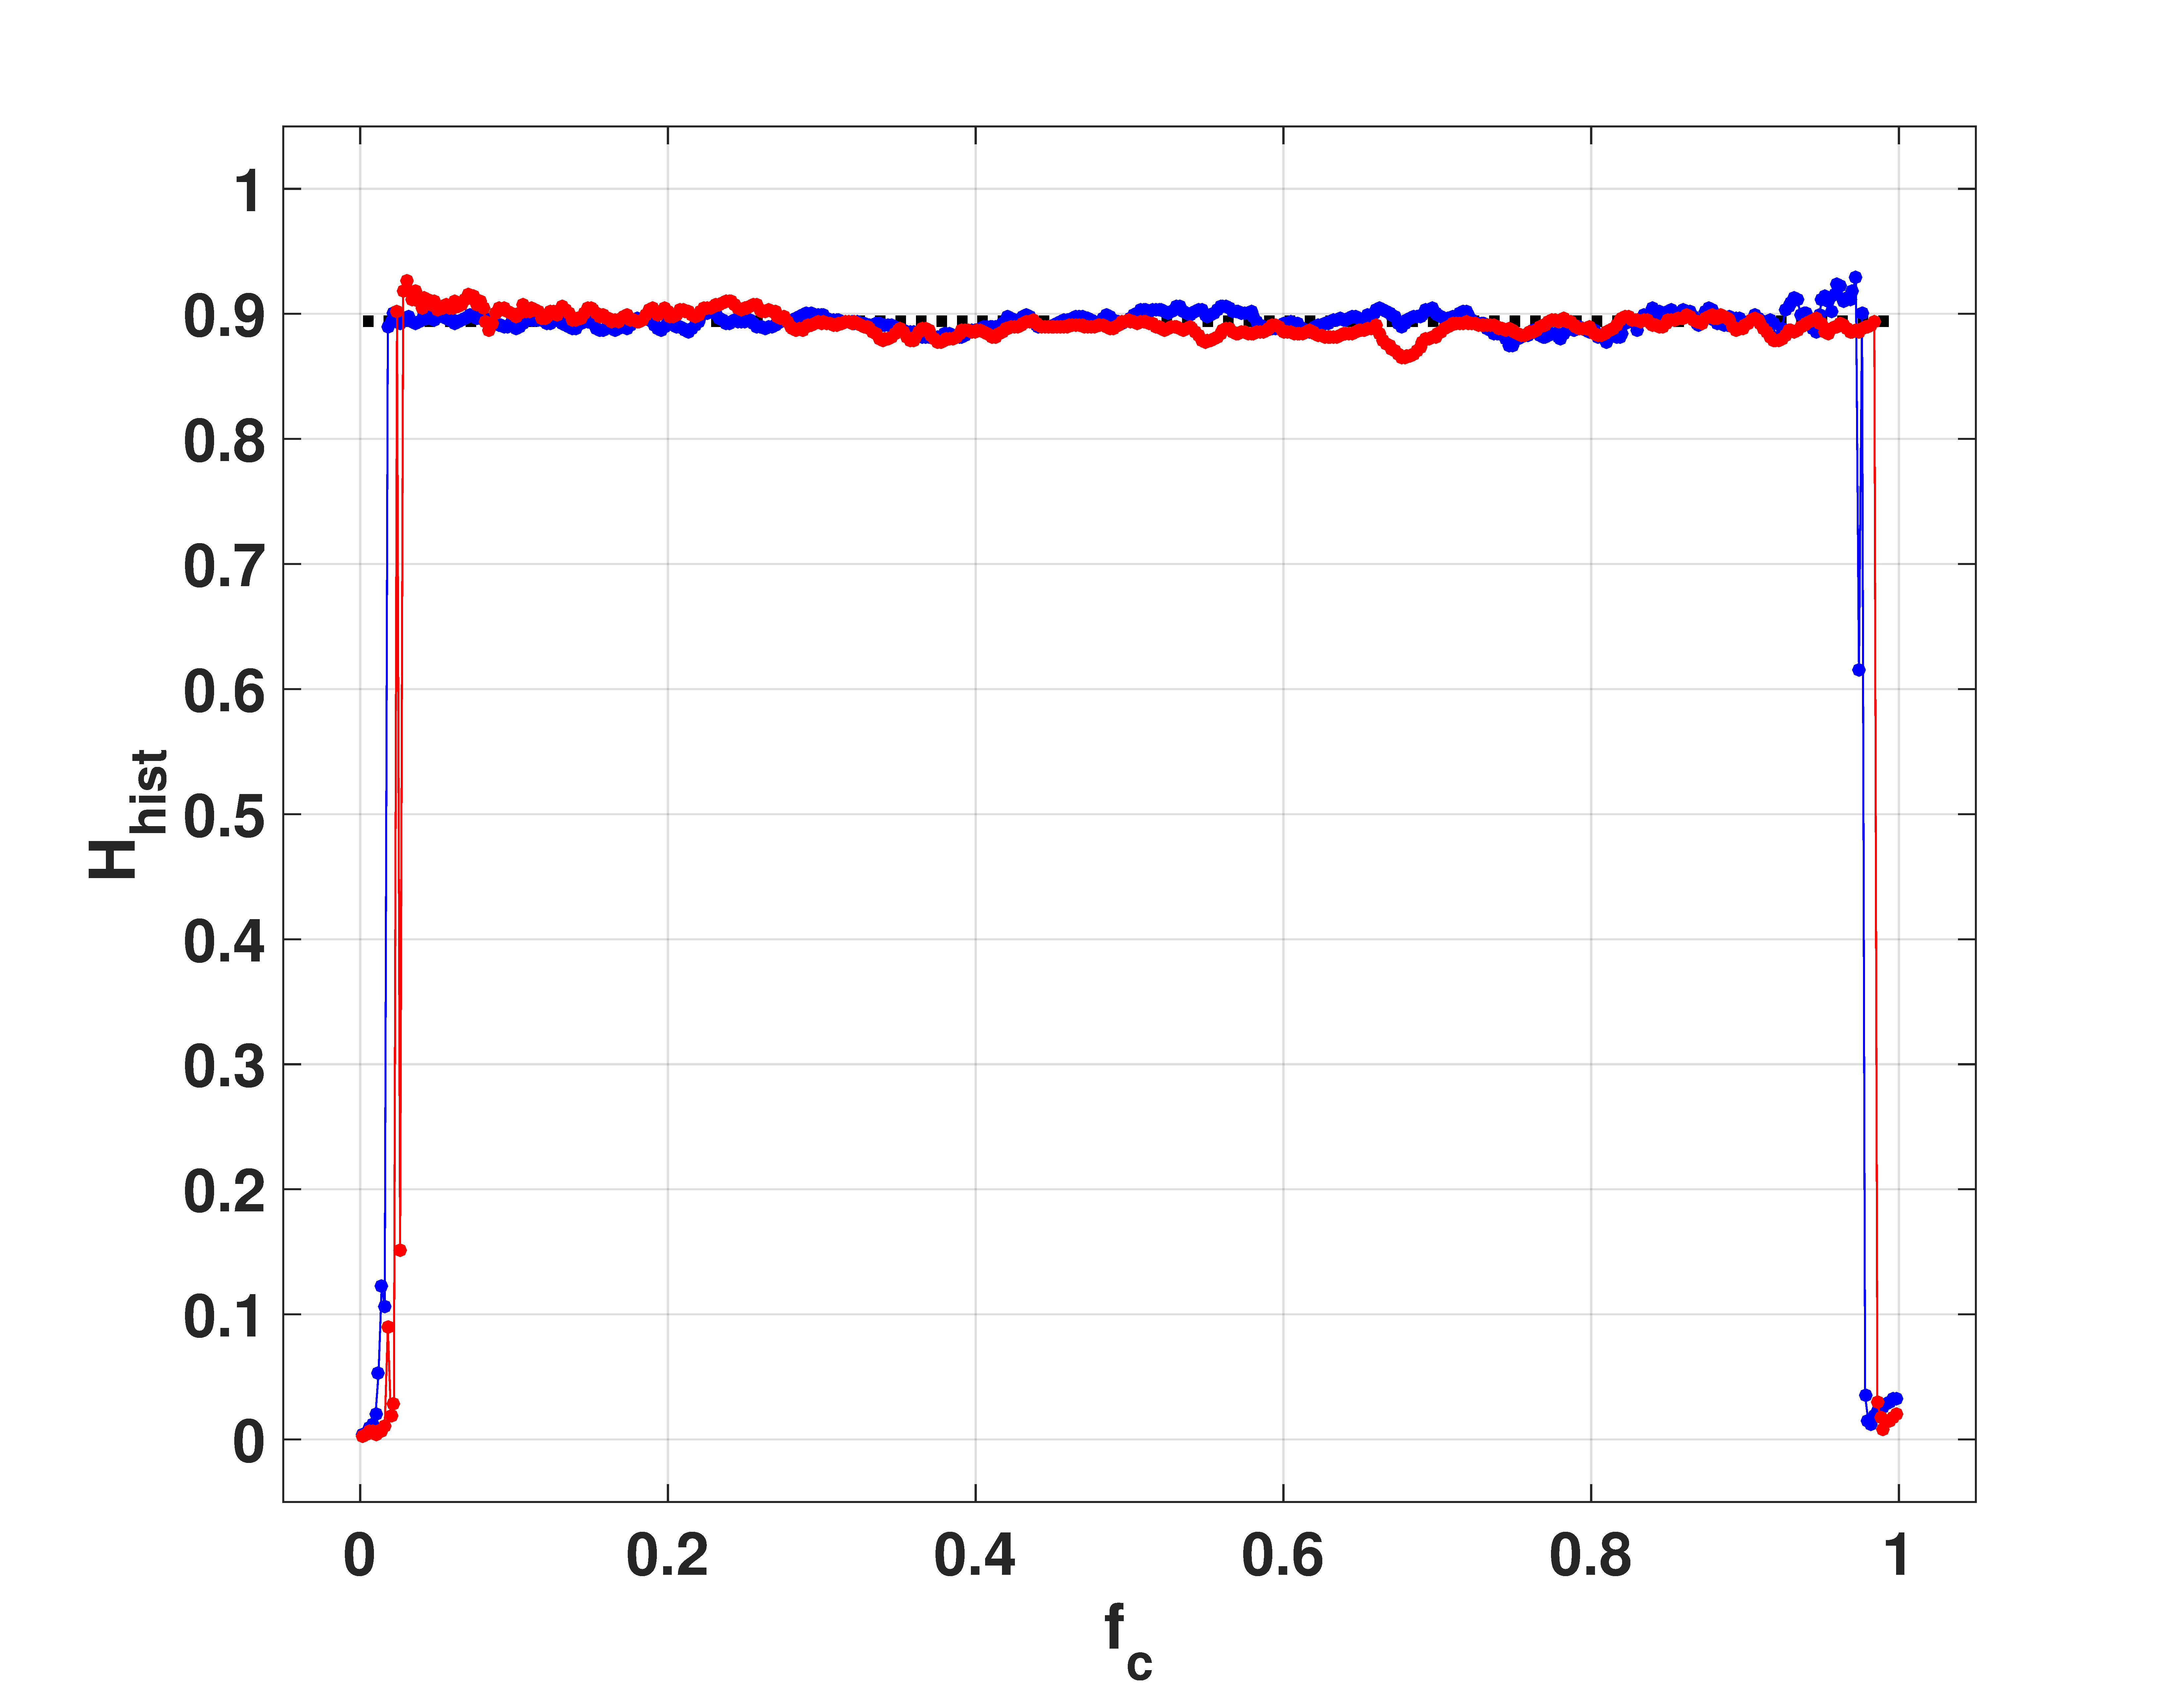
\includegraphics[width=\textwidth]{RuidoEllip_Hhist}
        \caption{Entropía de valores normalizada}
        \label{subfig:ellip_Hhist}
    \end{subfigure}
    ~ %add desired spacing between images, e. g. ~, \quad, \qquad, \hfill etc. 
      %(or a blank line to force the subfigure onto a new line)
    \begin{subfigure}[t]{0.32\textwidth}
        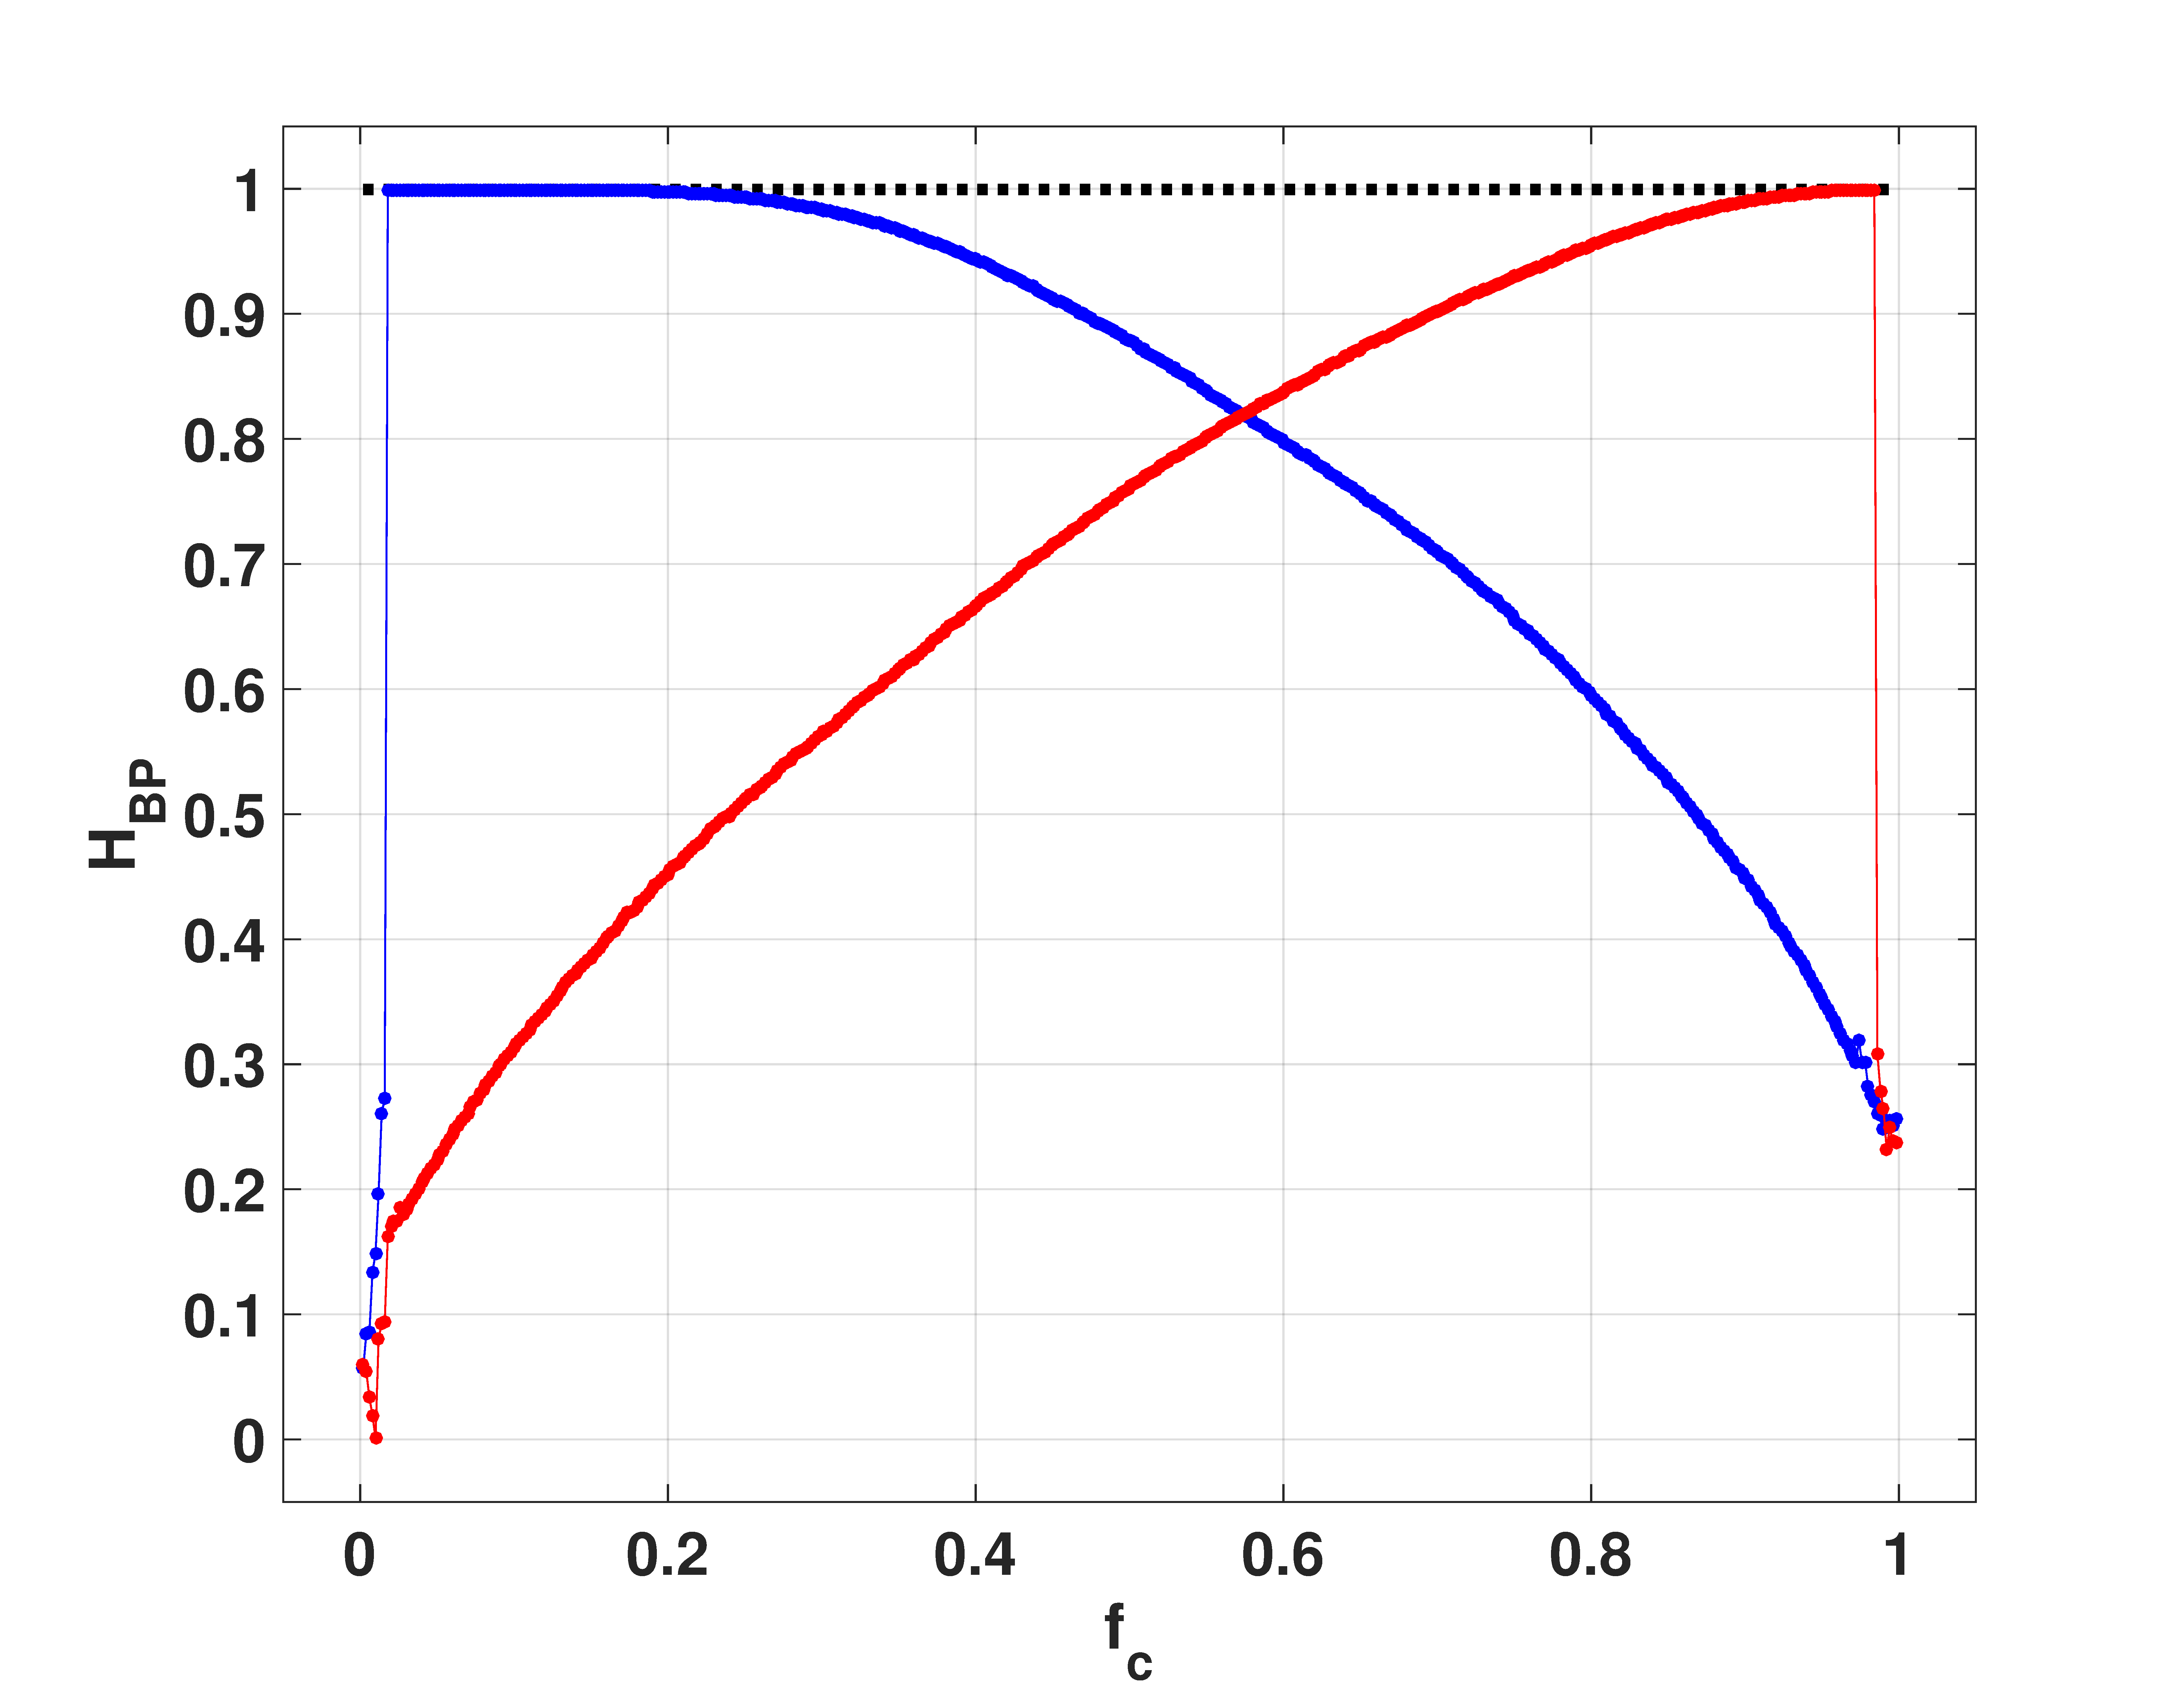
\includegraphics[width=\textwidth]{RuidoEllip_Hbp}
        \caption{Entropía de patrones de orden normalizada}
        \label{subfig:ellip_Hbp}
    \end{subfigure}
    ~ %add desired spacing between images, e. g. ~, \quad, \qquad, \hfill etc. 
    %(or a blank line to force the subfigure onto a new line)
    \begin{subfigure}[t]{0.32\textwidth}
        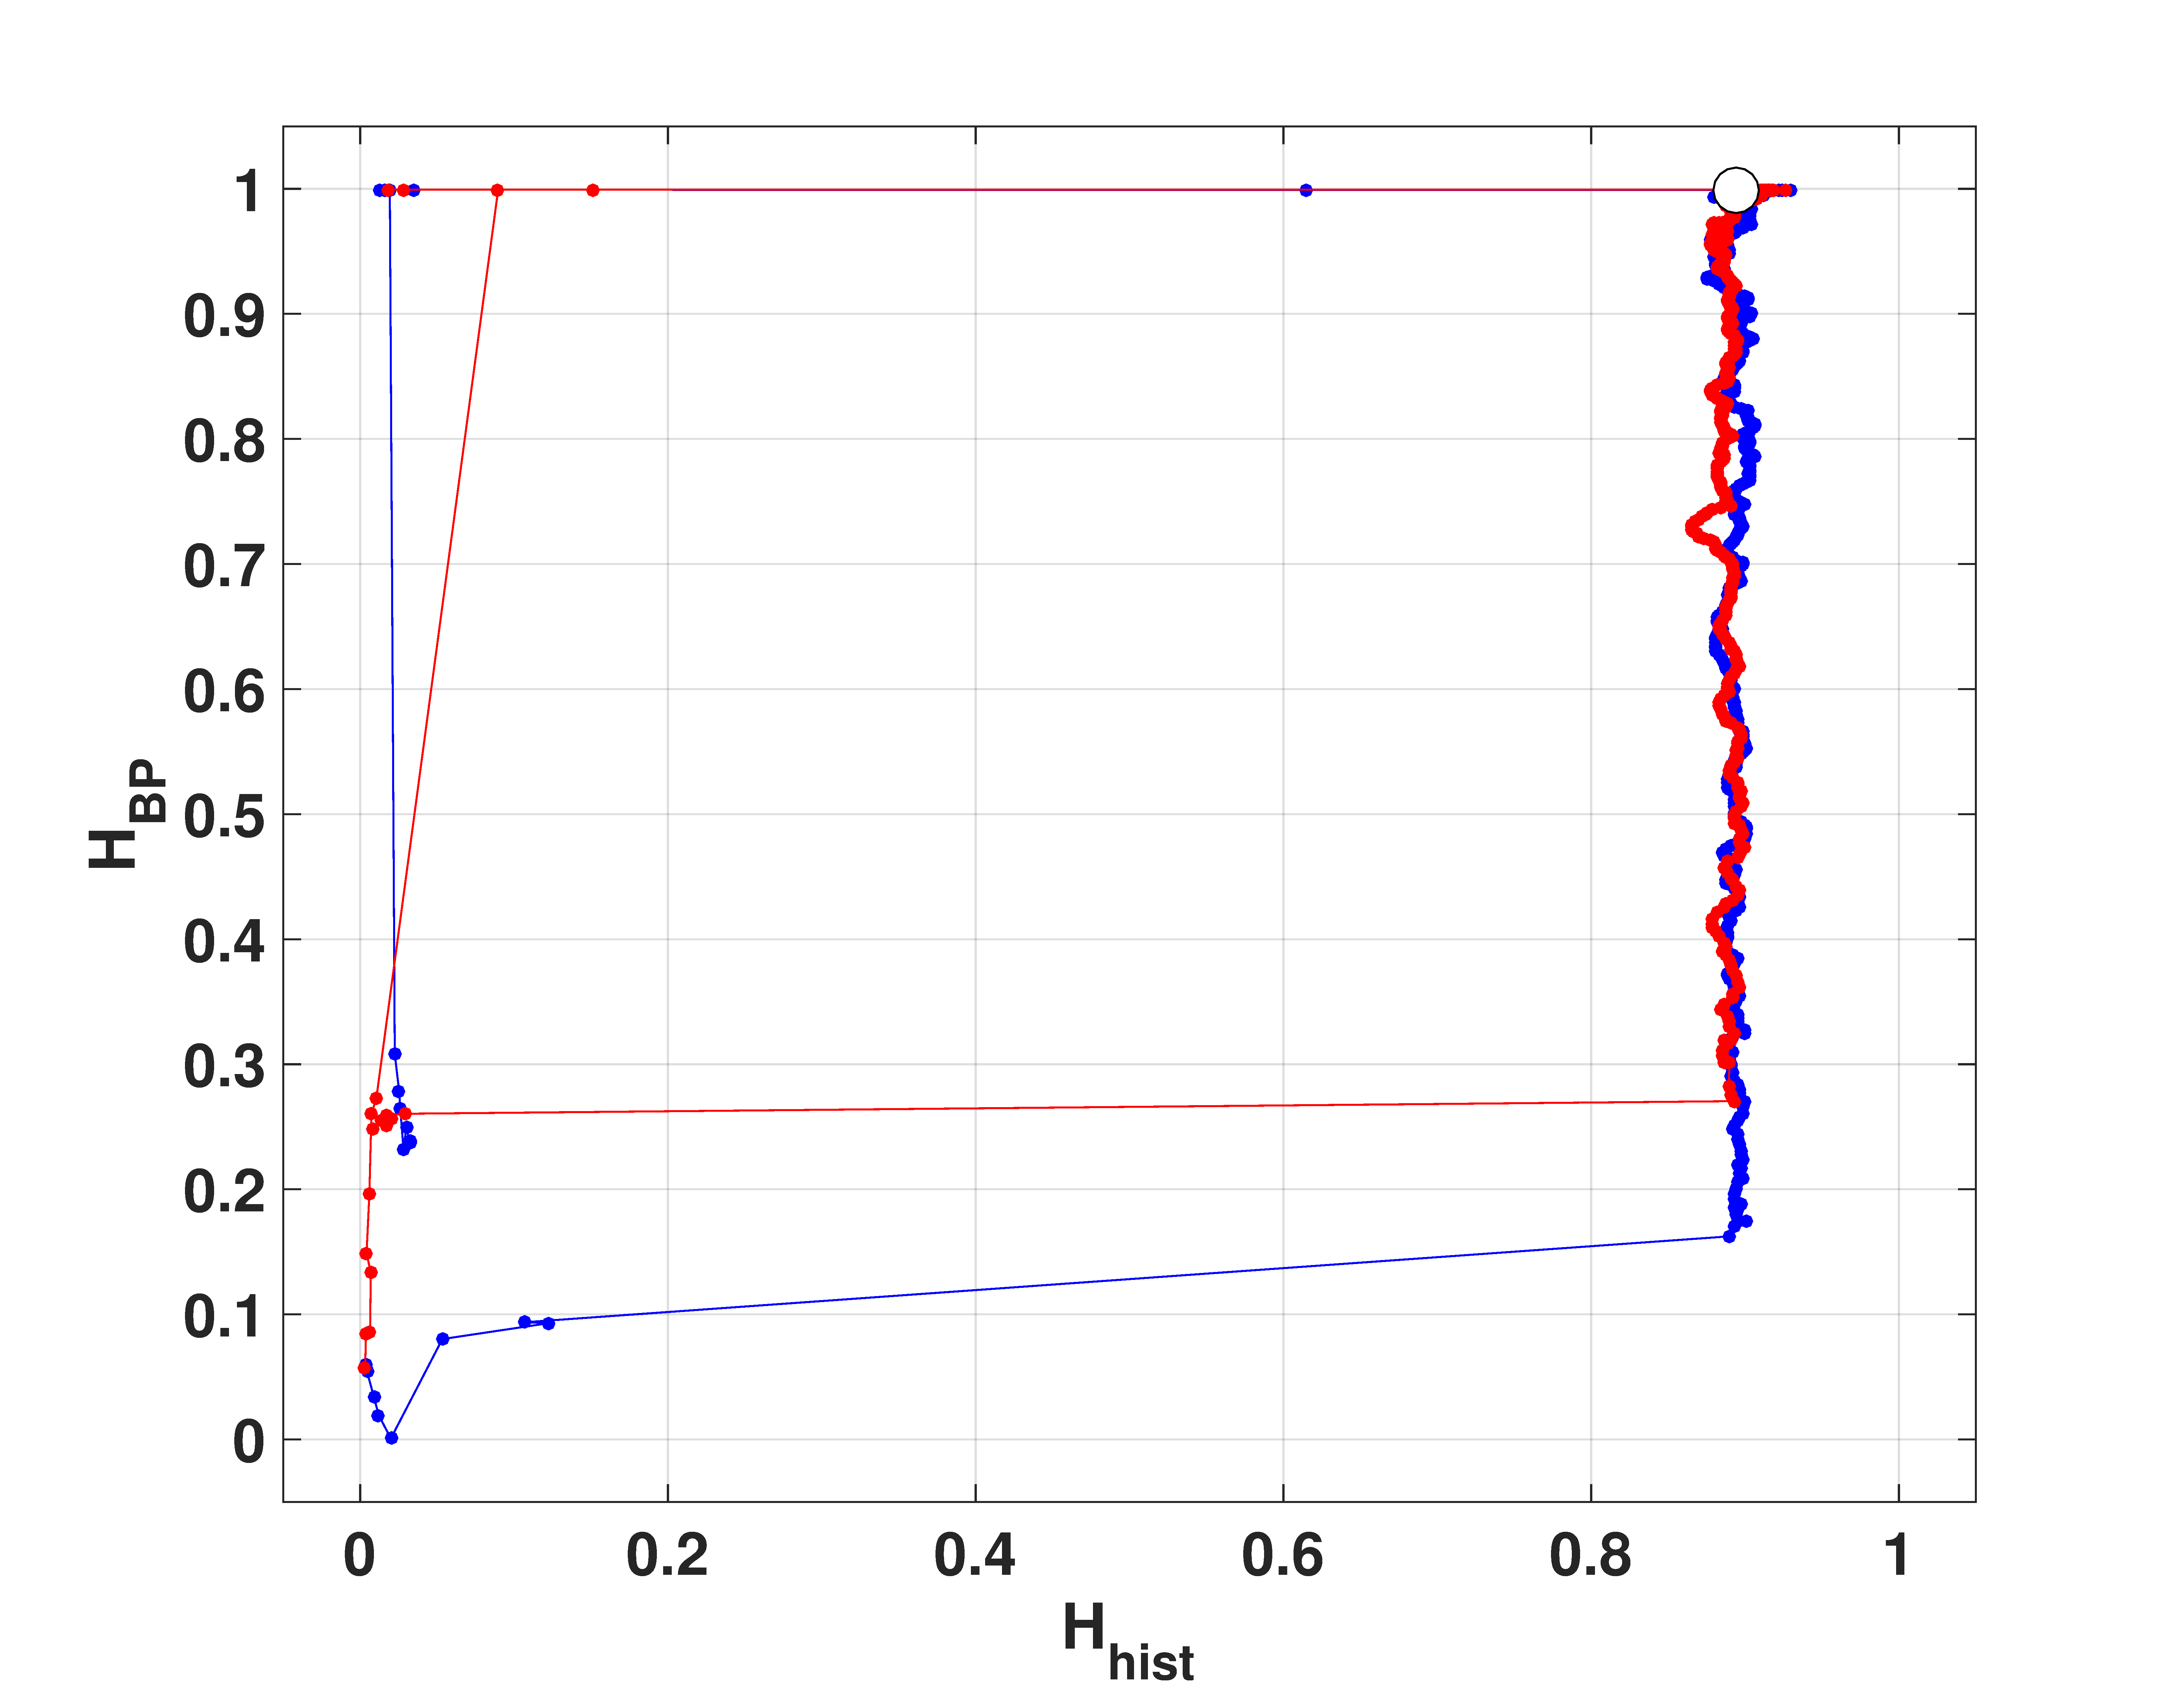
\includegraphics[width=\textwidth]{RuidoEllip_Hbp_Hhist}
        \caption{Plano deoble entropía}
        \label{subfig:ellip_HbpHhist}
    \end{subfigure}
    \caption{Cuantificadores calculados sobre la salida del filtro elíptico cuando se ingresa con ruido blanco gaussiano.}\label{fig:ellip}
\end{figure}

En la figura \ref{fig:ideal} se muestran los resultados del mismo procedimiento pero cuando se aplica un filtro ideal.
El comportamiento de los cuantificadores es igual al del filtro elíptico en todos los casos con la diferencia que el método no diverge cuando $f_c\to1$ o $f_c\to0$.
Pueden verse por lo tanto los valores que arrojan los cuantificadores en los extremos de la frecuencia de corte.
La entropía no causal de la figura \ref{subfig:ideal_Hhist} aumenta levemente en los extremos, en donde el histograma de valores deja de tener una distribución gaussiana y se aplana levemente.
También puede verse en \ref{subfig:ideal_Hbp} que la entropía de valores $H_{BP}\to0,15$ cuando $f_c\to0$ para el pasa-bajos (rojo) y para el pasa-altos (azul) $H_{BP}\to0,22$ cuando $f_c\to1$.
En este caso es fácil comparar la sensibilidad al filtrado de ambos cuantificadores, en el plano doble entropía de la figura \ref{subfig:ideal_HbpHhist}.
El círculo blanco muestra la posición en este plano cuando ningún filtro es aplicado, podemos ver que el apartamiento en el eje vertical aumenta a medida que la serie es filtrada, mientras que no se aparta en el sentido horizontal.
Esto muestra que la sensibilidad al filtrado de $H_{BP}$ es mucho mayor que la de $H_{hist}$.
%
\begin{figure}[h]
    \centering
    \begin{subfigure}[t]{0.32\textwidth}
        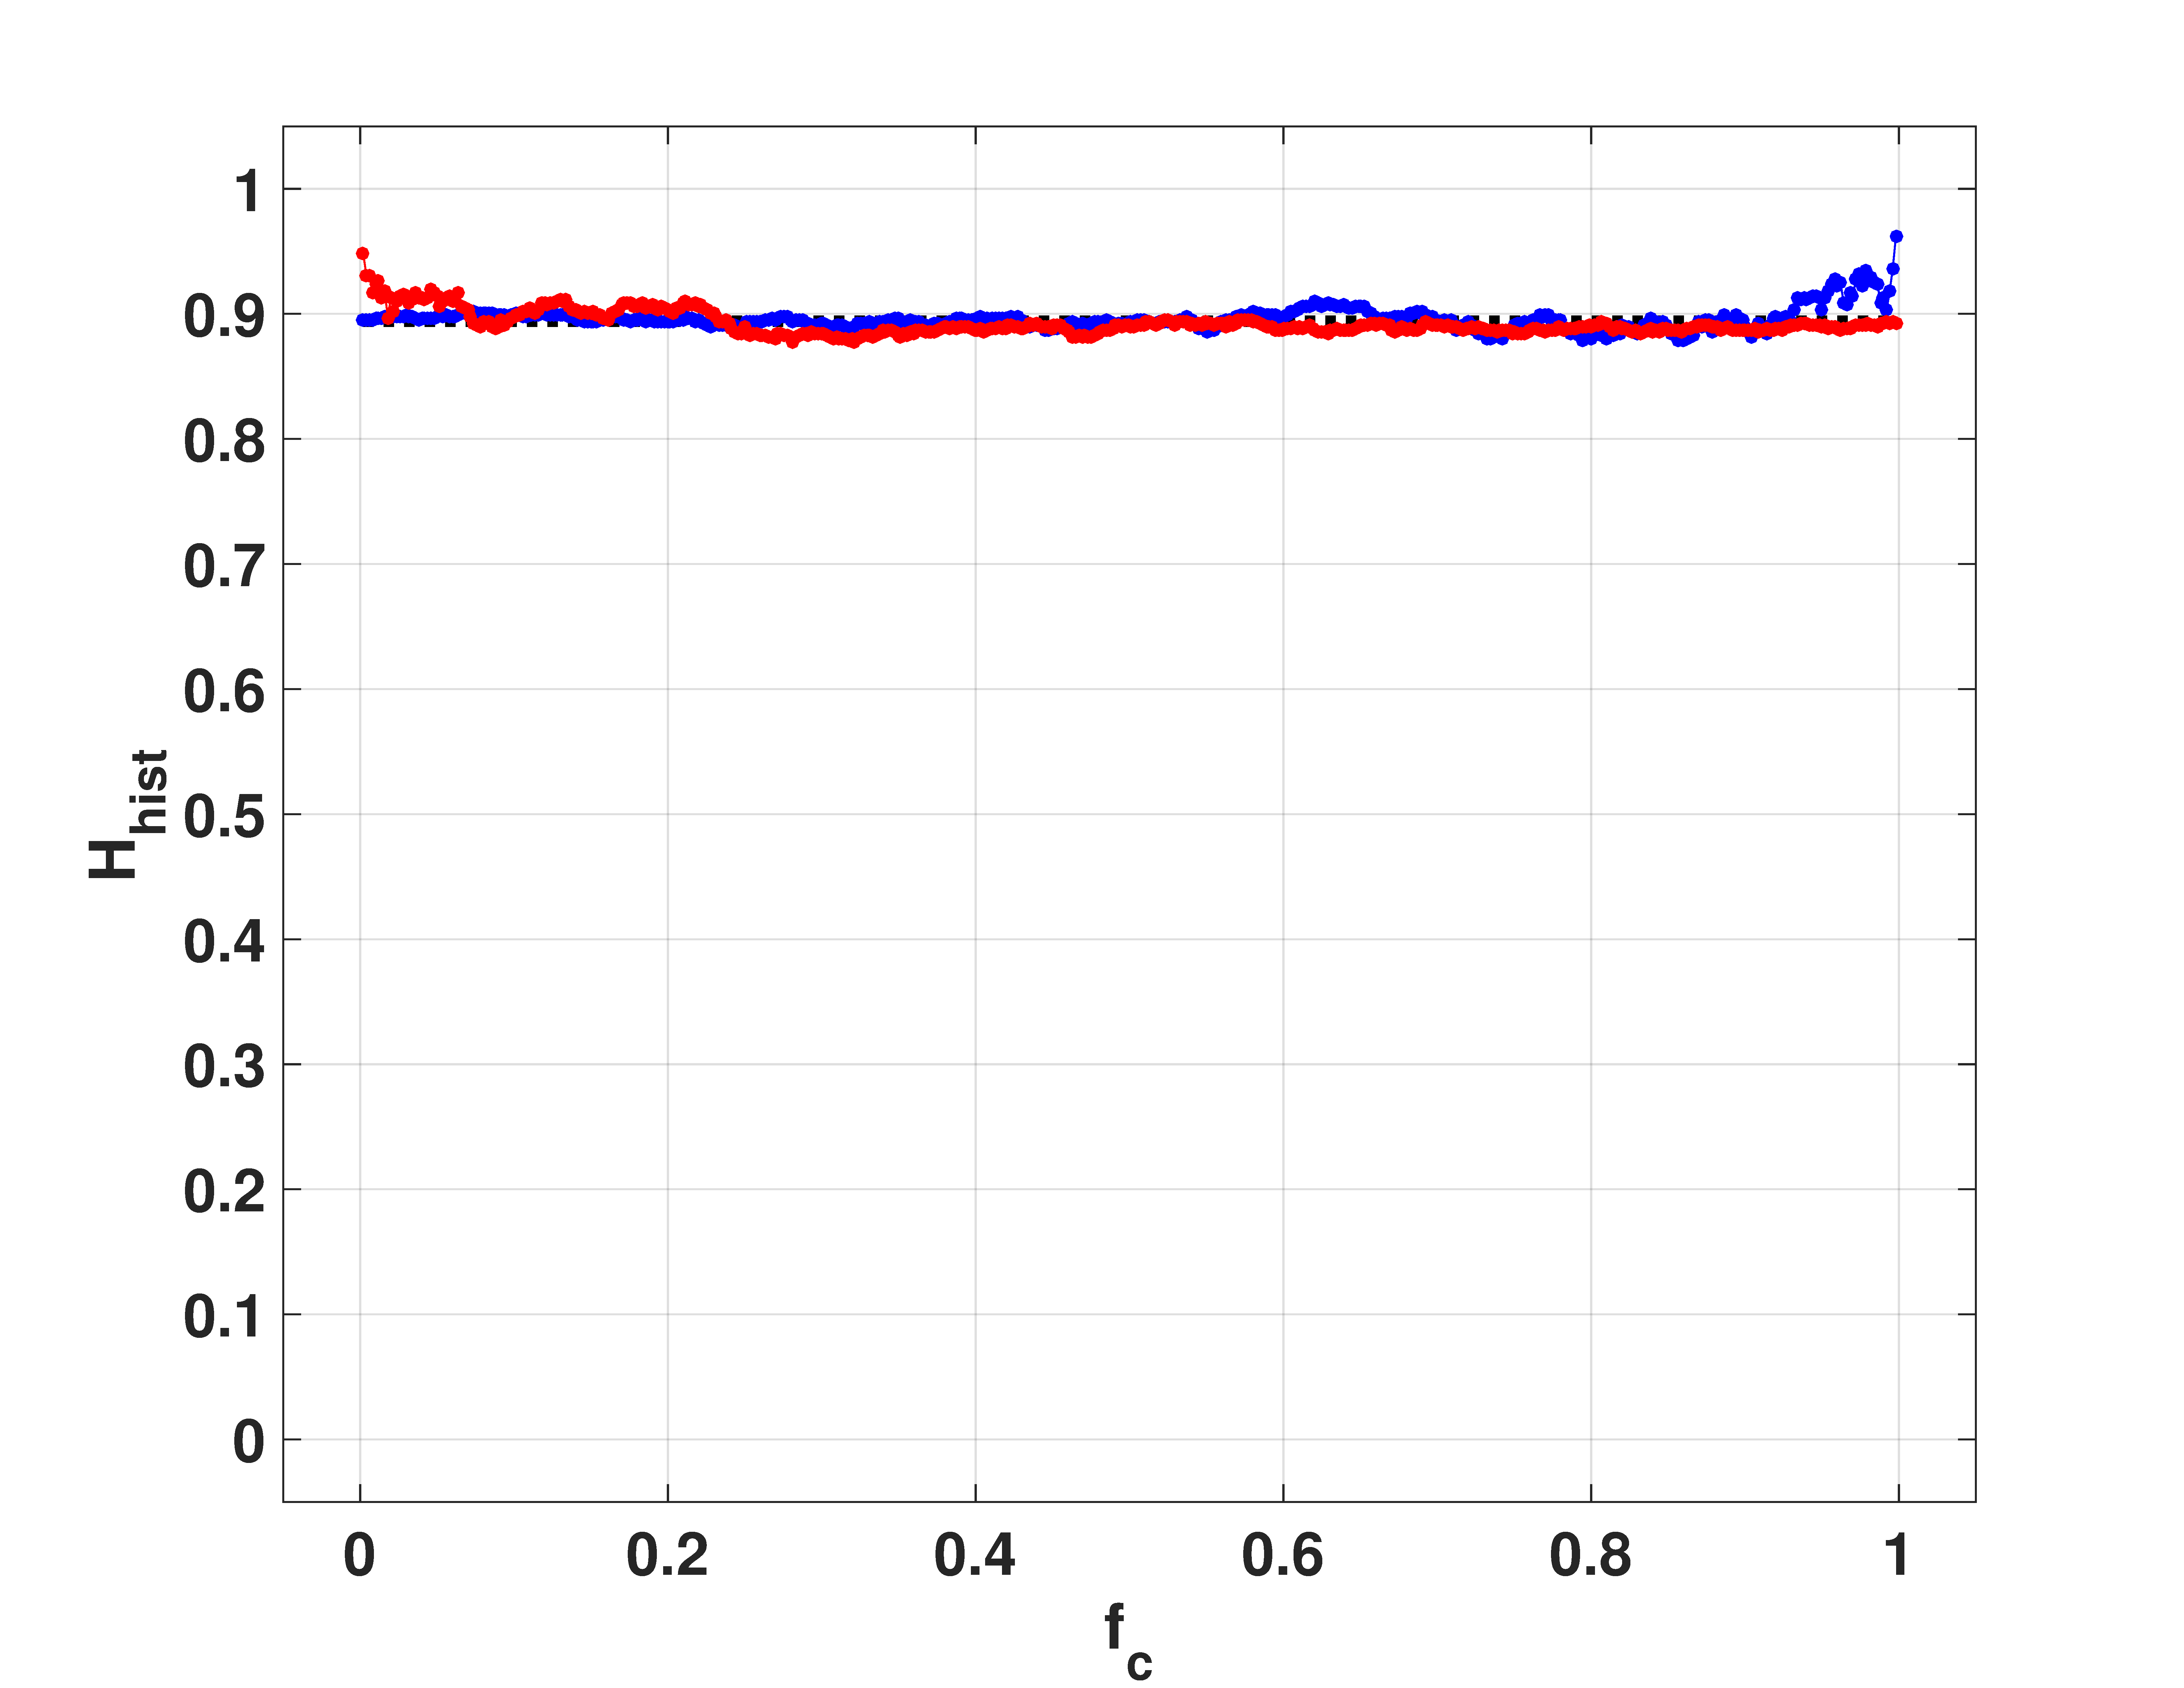
\includegraphics[width=\textwidth]{Ruido_Hhist}
        \caption{Entropía de valores normalizada}
        \label{subfig:ideal_Hhist}
    \end{subfigure}
    ~ %add desired spacing between images, e. g. ~, \quad, \qquad, \hfill etc. 
      %(or a blank line to force the subfigure onto a new line)
    \begin{subfigure}[t]{0.32\textwidth}
        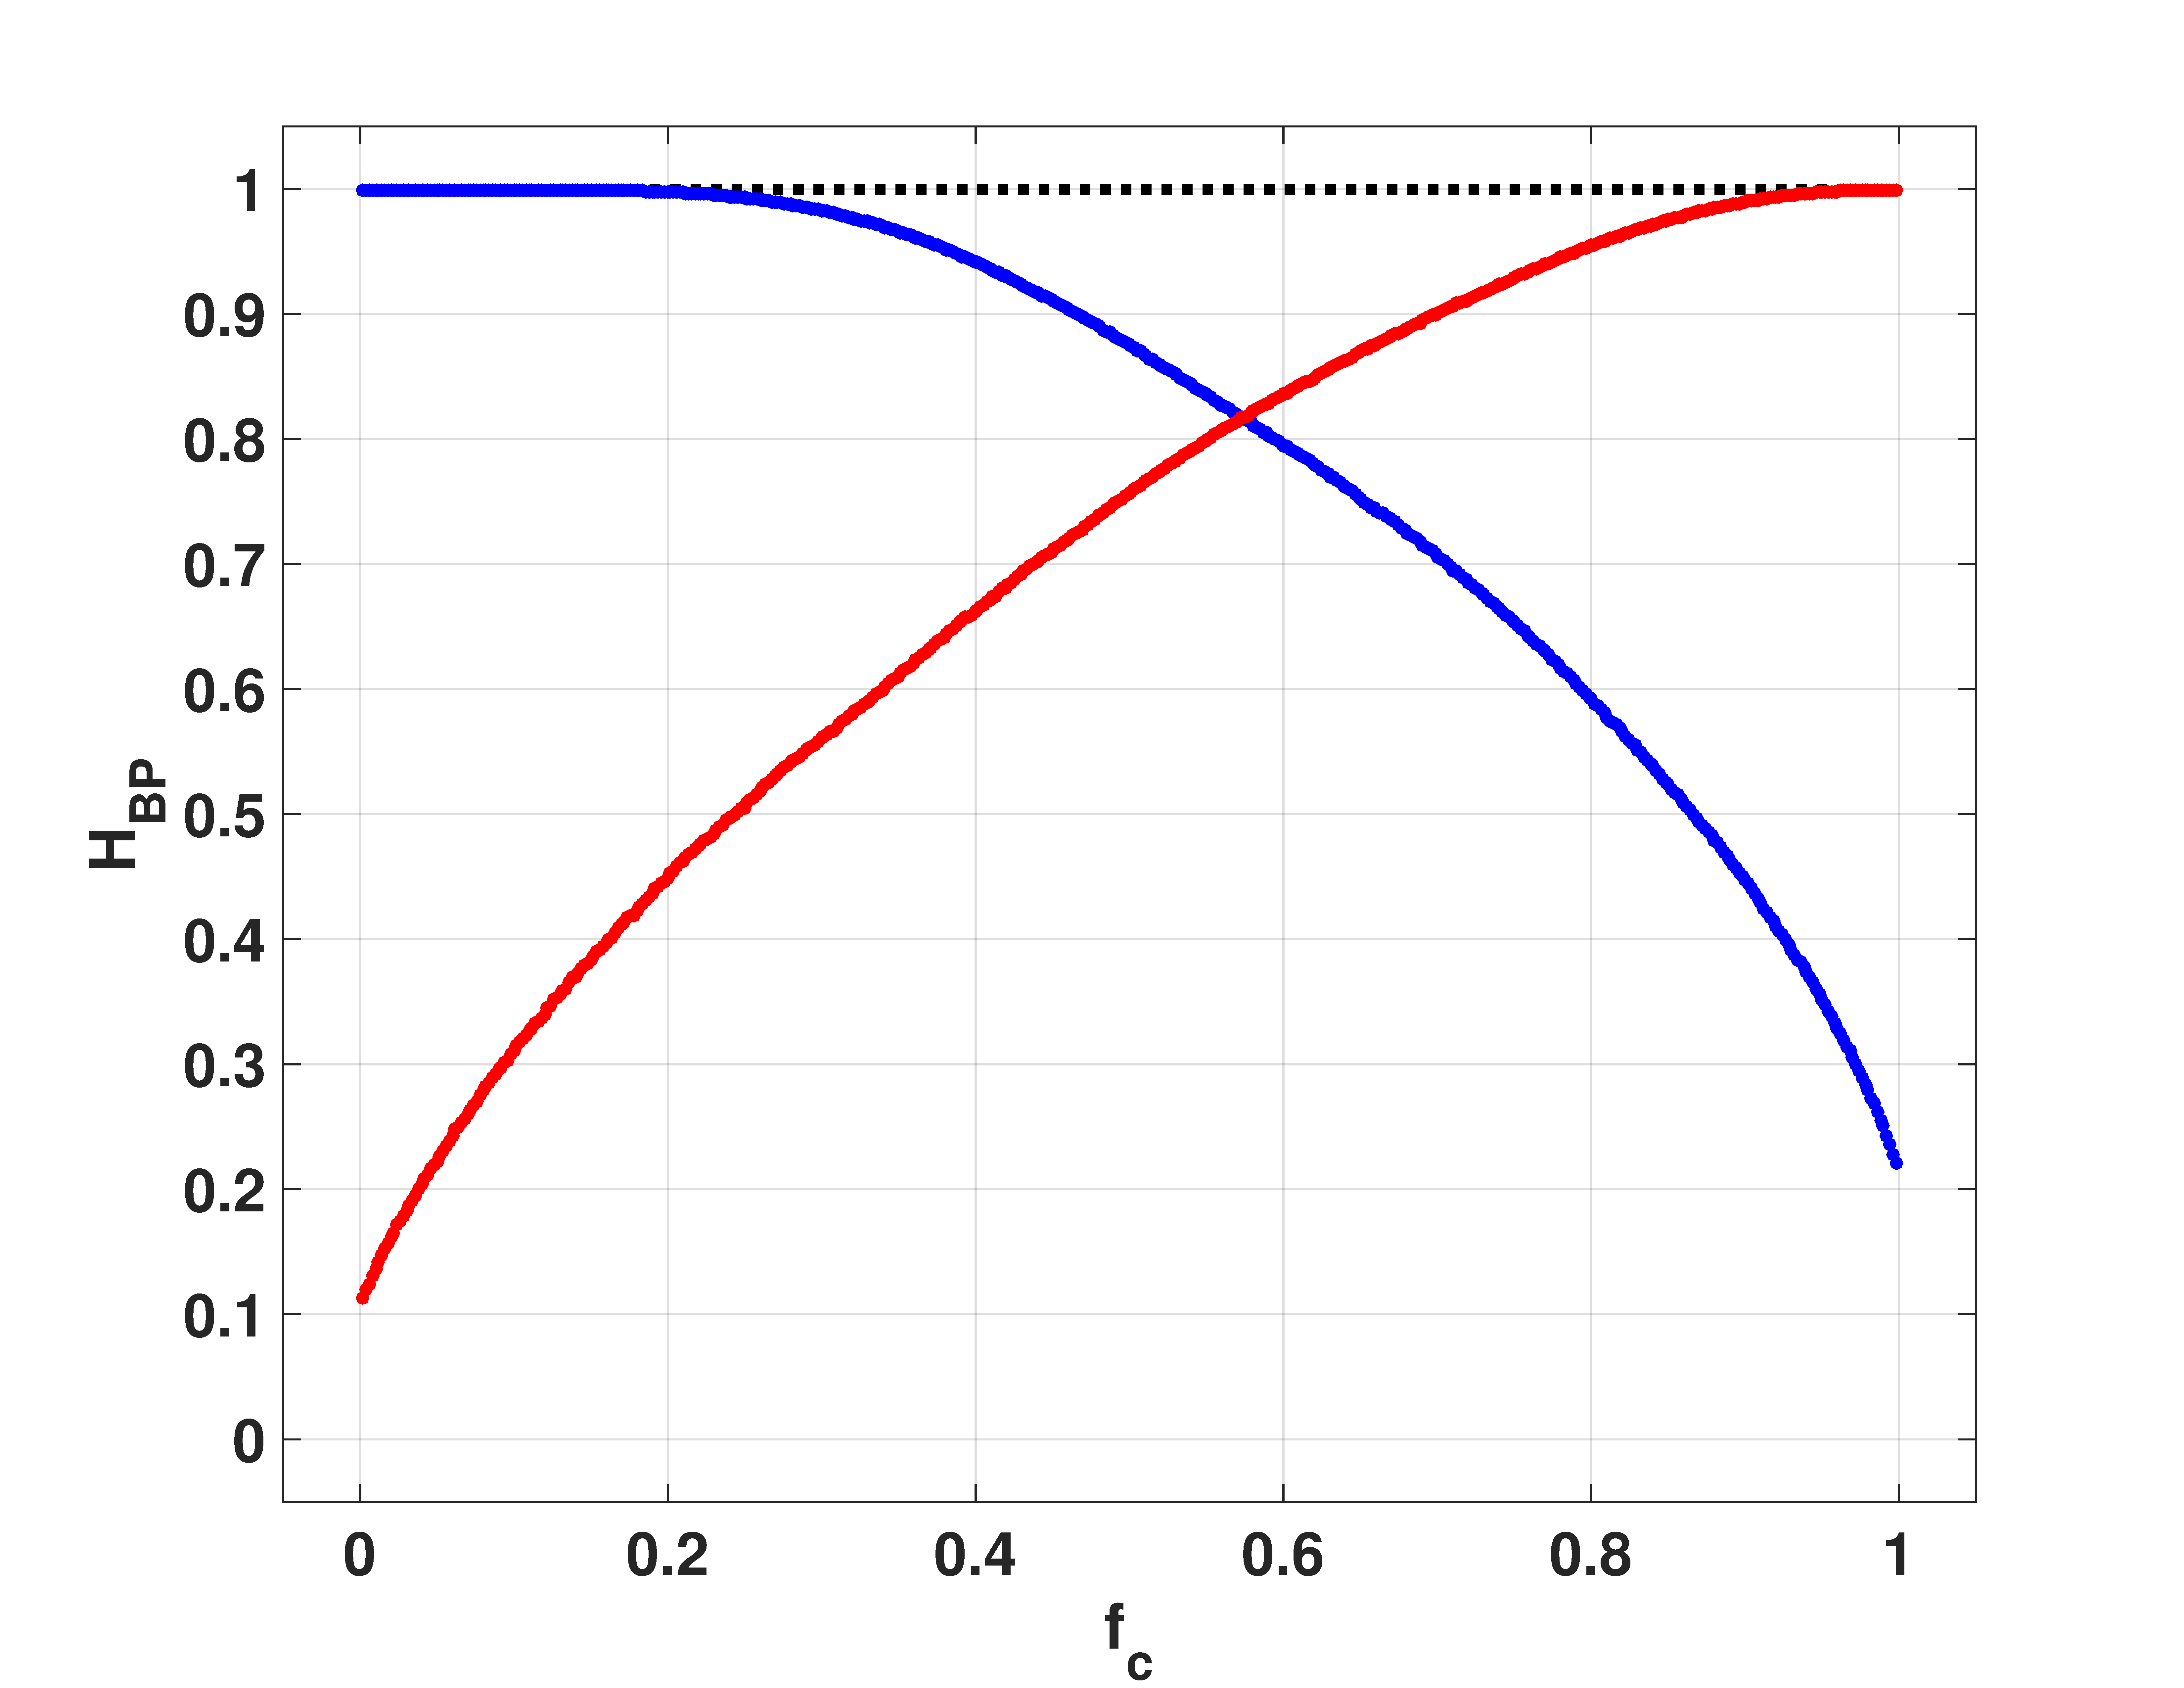
\includegraphics[width=\textwidth]{Ruido_Hbp}
        \caption{Entropía de patrones de orden normalizada}
        \label{subfig:ideal_Hbp}
    \end{subfigure}
    ~ %add desired spacing between images, e. g. ~, \quad, \qquad, \hfill etc. 
    %(or a blank line to force the subfigure onto a new line)
    \begin{subfigure}[t]{0.32\textwidth}
        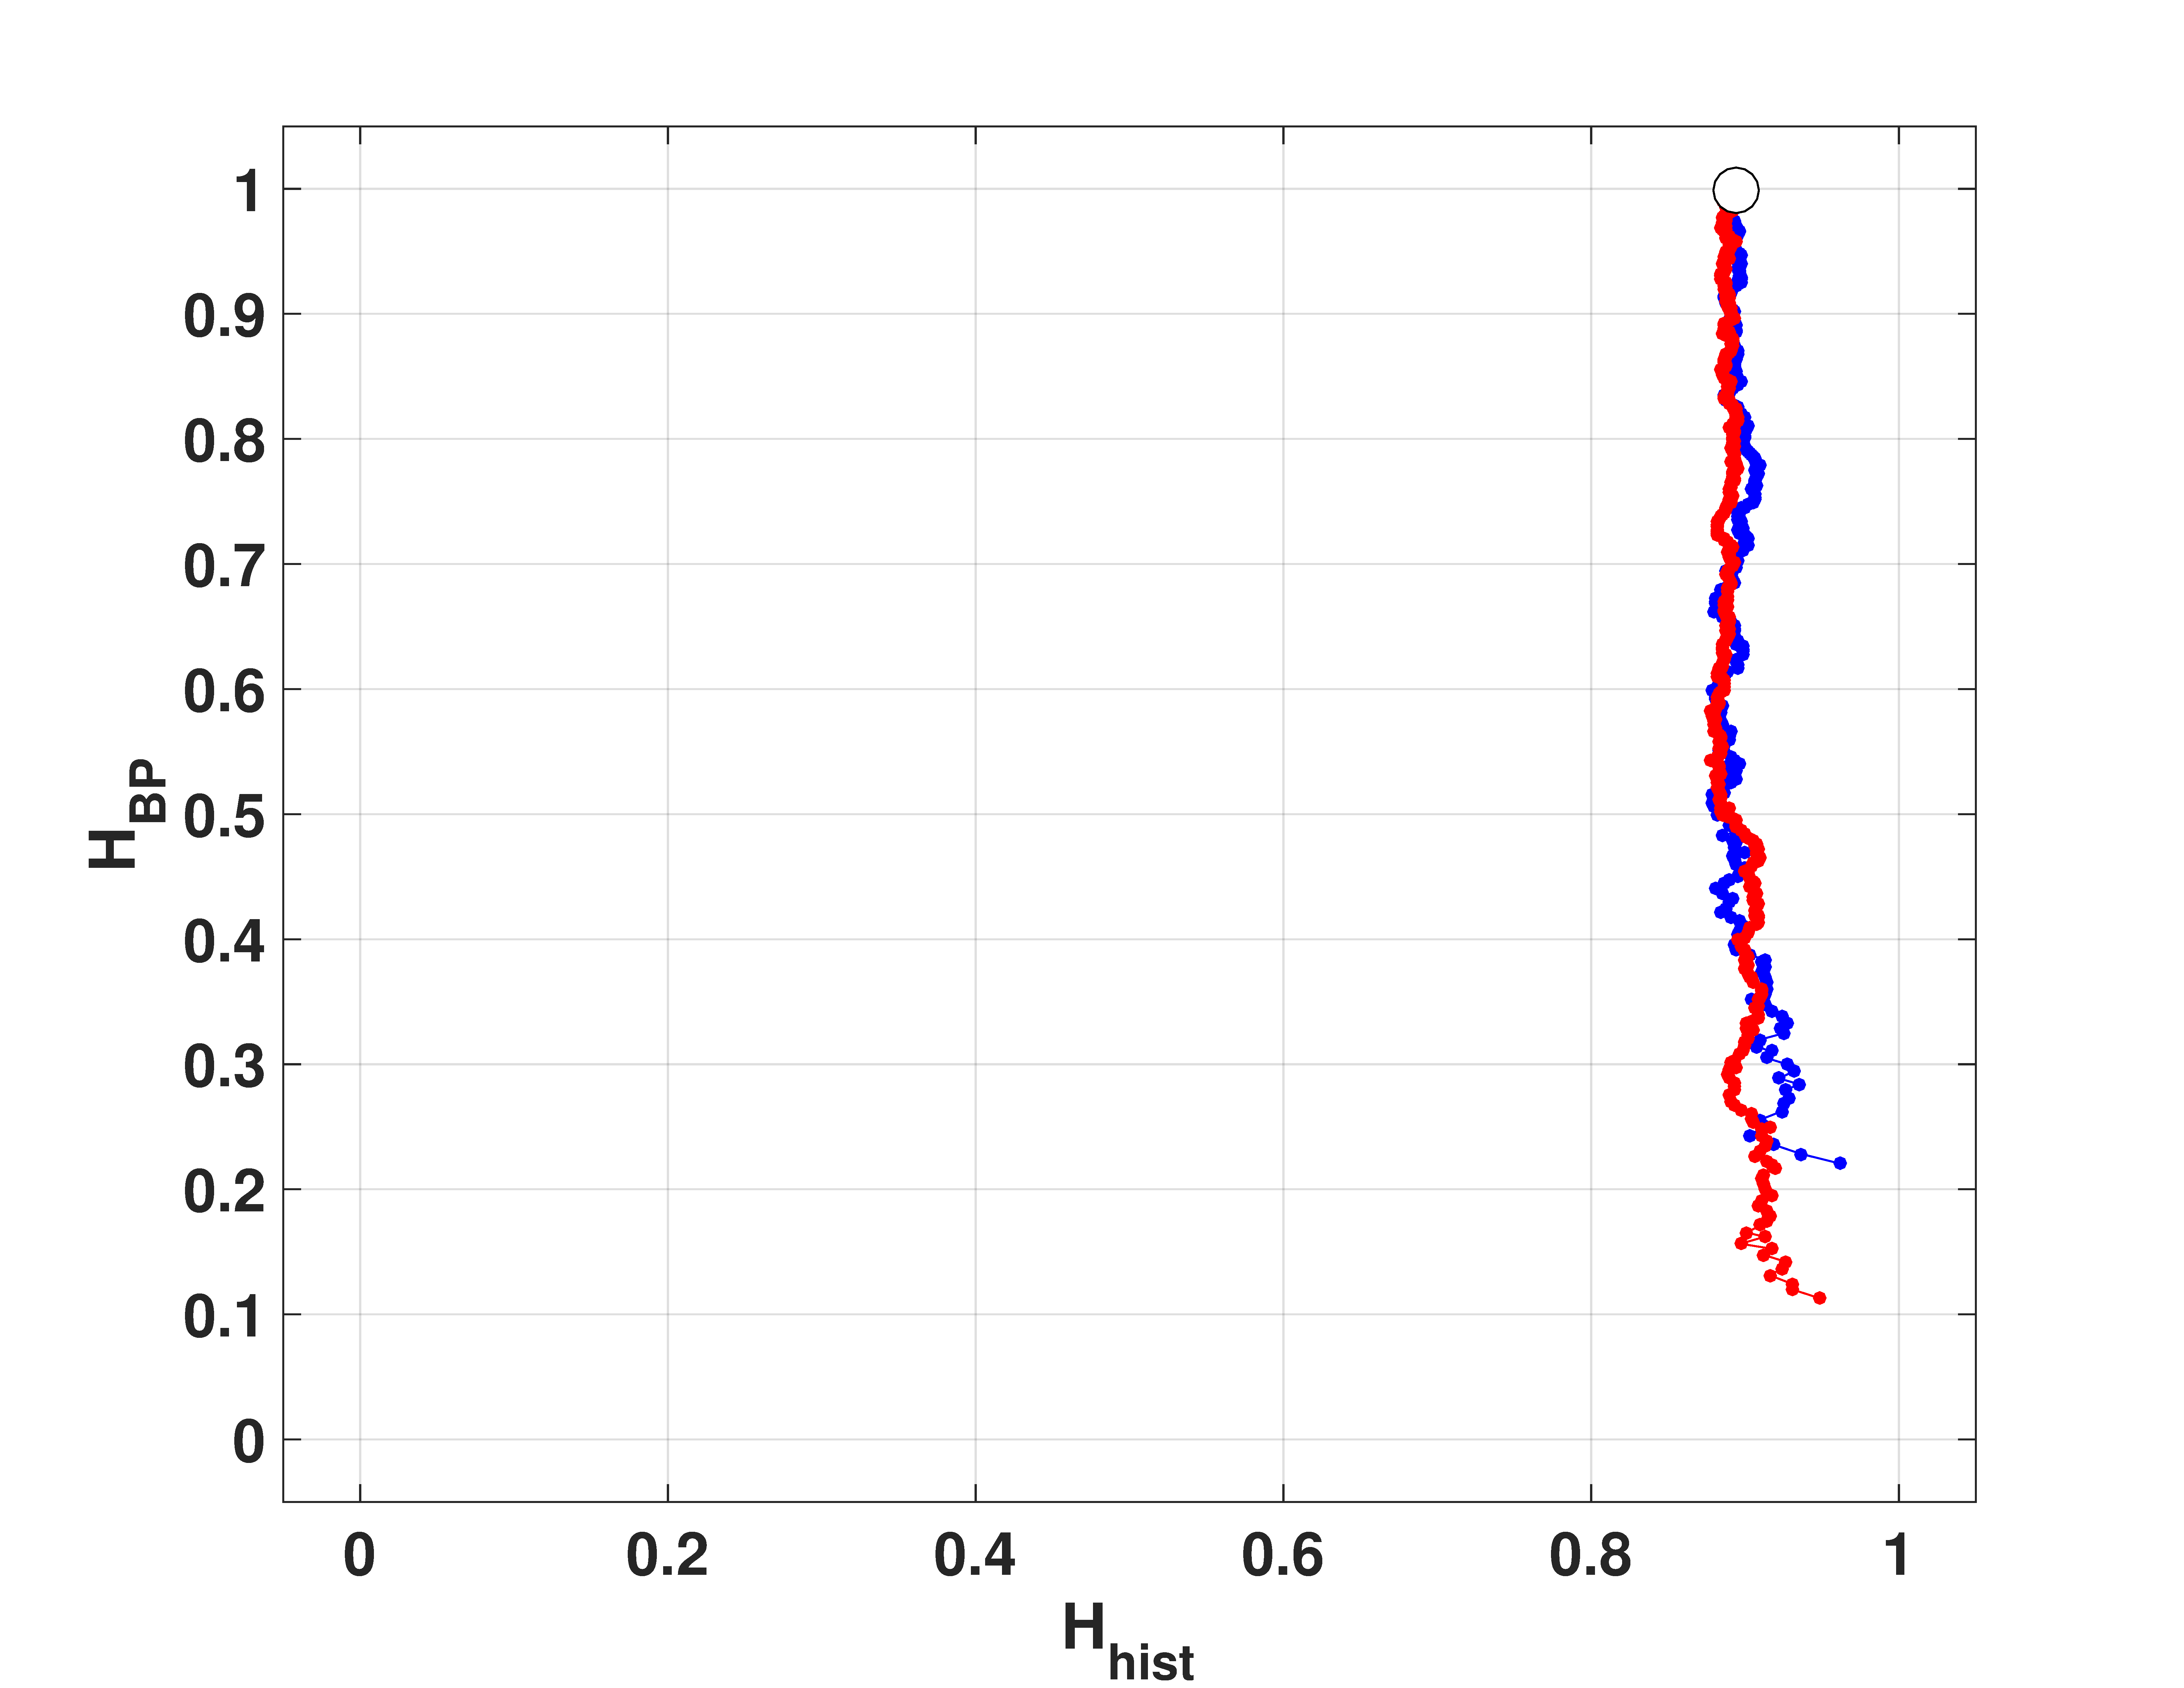
\includegraphics[width=\textwidth]{Ruido_Hbp_Hhist}
        \caption{Plano deoble entropía}
        \label{subfig:ideal_HbpHhist}
    \end{subfigure}
    \caption{Cuantificadores calculados sobre la salida del filtro ideal cuando se ingresa con ruido blanco gaussiano.}\label{fig:ideal}
\end{figure}

Para el sistema planteado no se necesita volver al dominio contínuo analógico, por lo que las dificultades mencionadas en la sección \ref{sec:filtrado} respecto al filtrado ideal (como ripple en las bandas de paso y rechazo) no aplican a este caso.
Por este motivo para esta serie de pruebas elegimos el filtro ideal, dado que presenta mejores resultados que el elíptico.

La primer señal determinística que se muestra es una senoidal de amplitud unitaria con período de $100$ muestras, los resultados pueden verse en la figura \ref{fig:Senoidal}.
Mientras la única componente espectral no es filtrada, el valor de la entropía de valores es $H_{hist}\approx0,57$ en la figura \ref{subfig:Senoidal_Hhist} y la entropía de patrones de orden $H_{BP}\approx0,16$ en la figura \ref{subfig:Senoidal_Hbp}.
Ambos cuantificadores caen a cero cuando la única componente espectral es filtrada, ya sea por el filtro pasa-bajos (azul) o por el pasa-altos (rojo).
El plano doble entropía muestra un punto en $\left(0,57;0,16\right)$ para la senoidal sin filtrar y otro en $\left(0;0\right)$ cuando la única componente espectral es filtrada.
%
\begin{figure}[h]
    \centering
    \begin{subfigure}[t]{0.32\textwidth}
        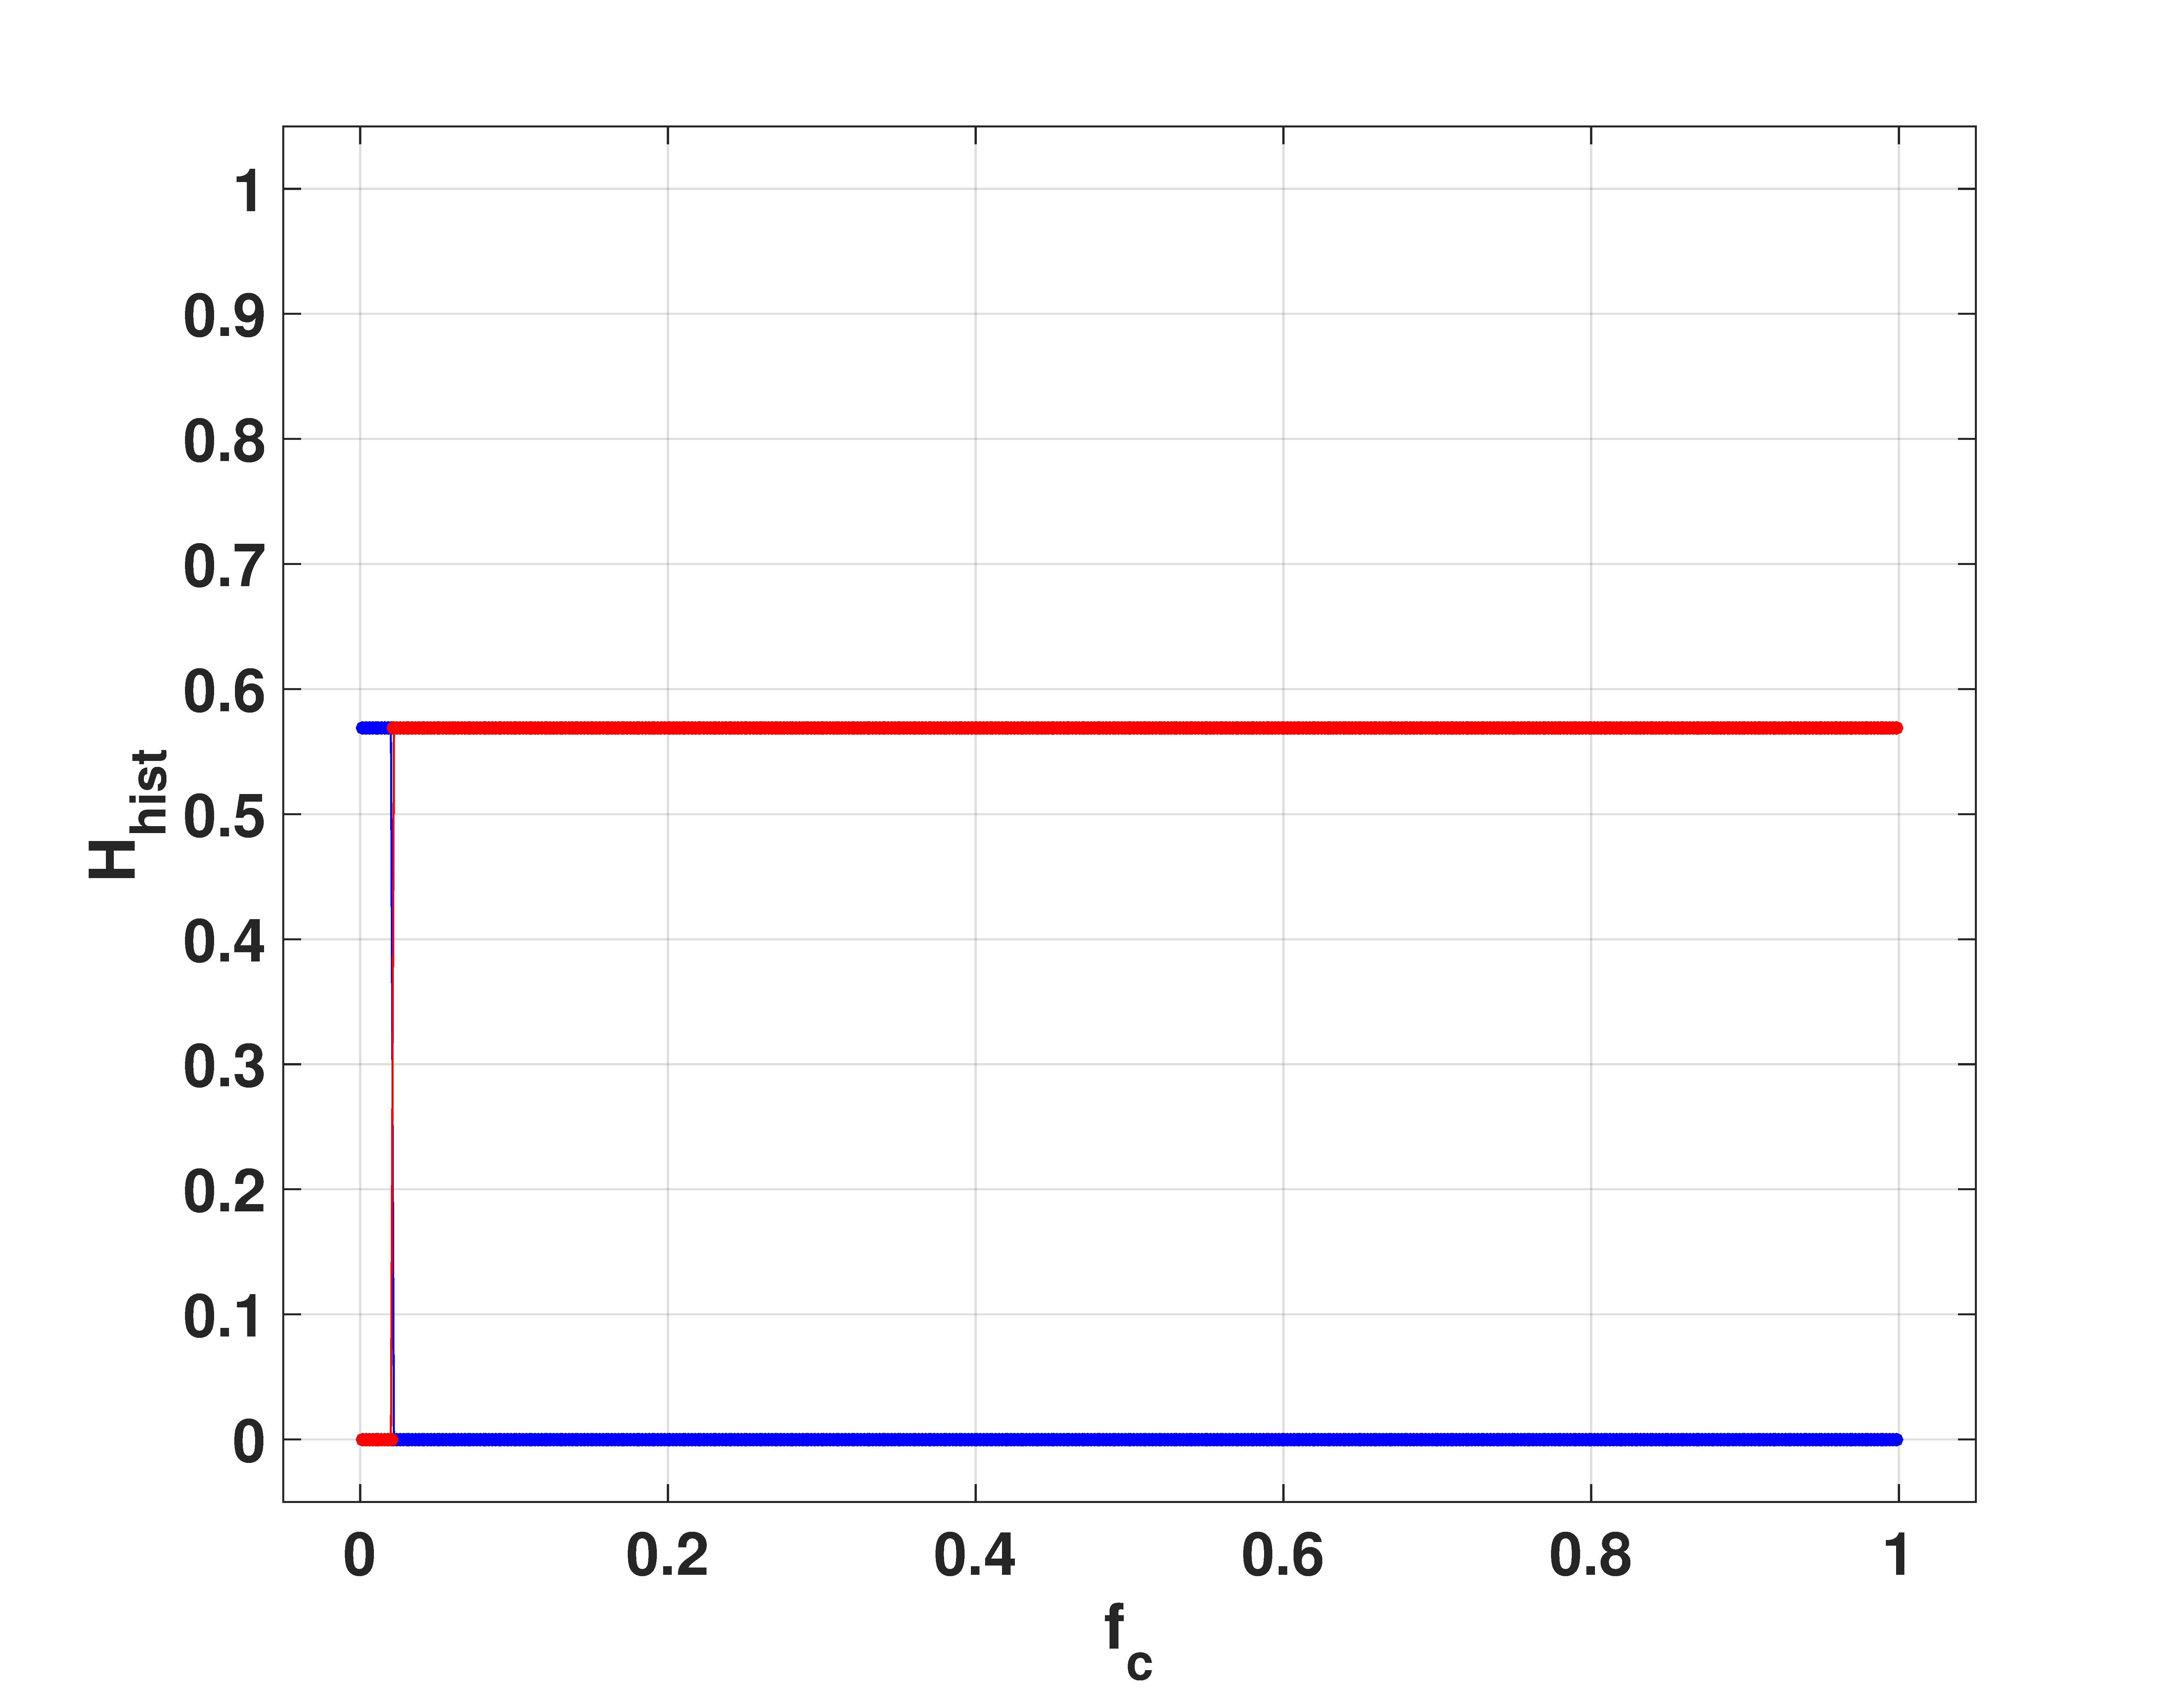
\includegraphics[width=\textwidth]{Senoidal_Hhist}
        \caption{Entropía de valores normalizada}
        \label{subfig:Senoidal_Hhist}
    \end{subfigure}
    ~ %add desired spacing between images, e. g. ~, \quad, \qquad, \hfill etc. 
      %(or a blank line to force the subfigure onto a new line)
    \begin{subfigure}[t]{0.32\textwidth}
        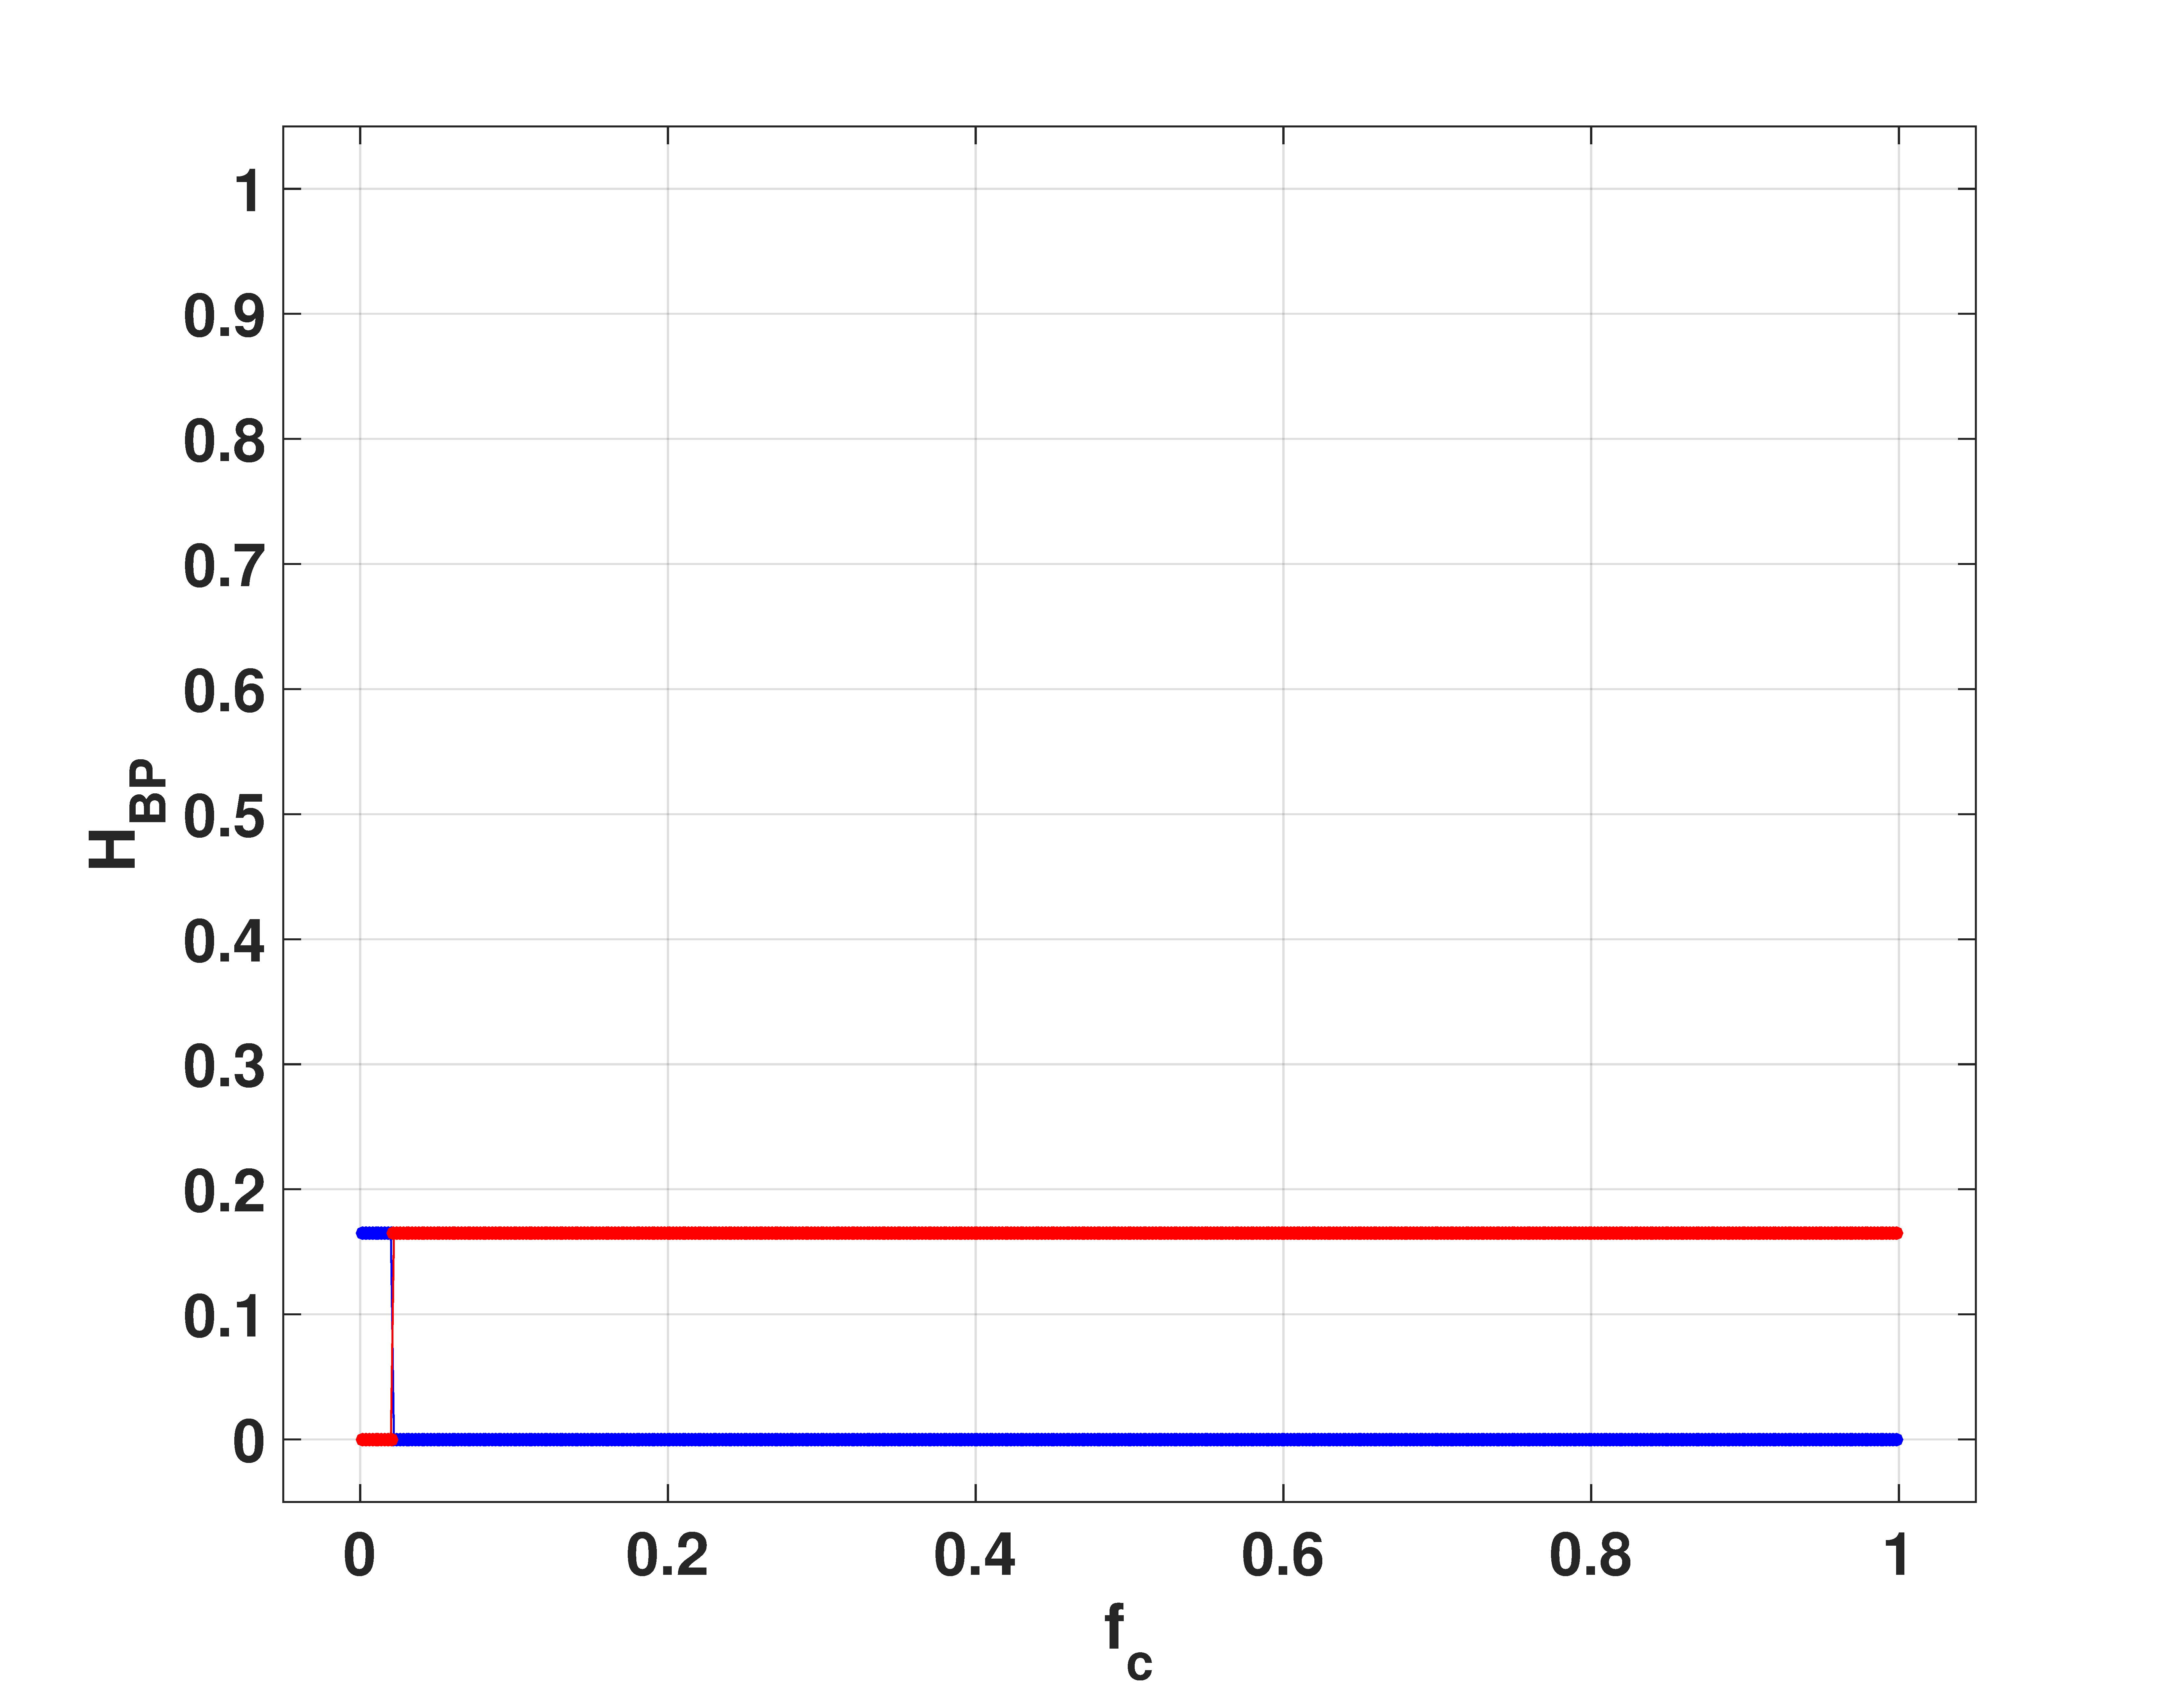
\includegraphics[width=\textwidth]{Senoidal_Hbp}
        \caption{Entropía de patrones de orden normalizada}
        \label{subfig:Senoidal_Hbp}
    \end{subfigure}
    ~ %add desired spacing between images, e. g. ~, \quad, \qquad, \hfill etc. 
    %(or a blank line to force the subfigure onto a new line)
    \begin{subfigure}[t]{0.32\textwidth}
        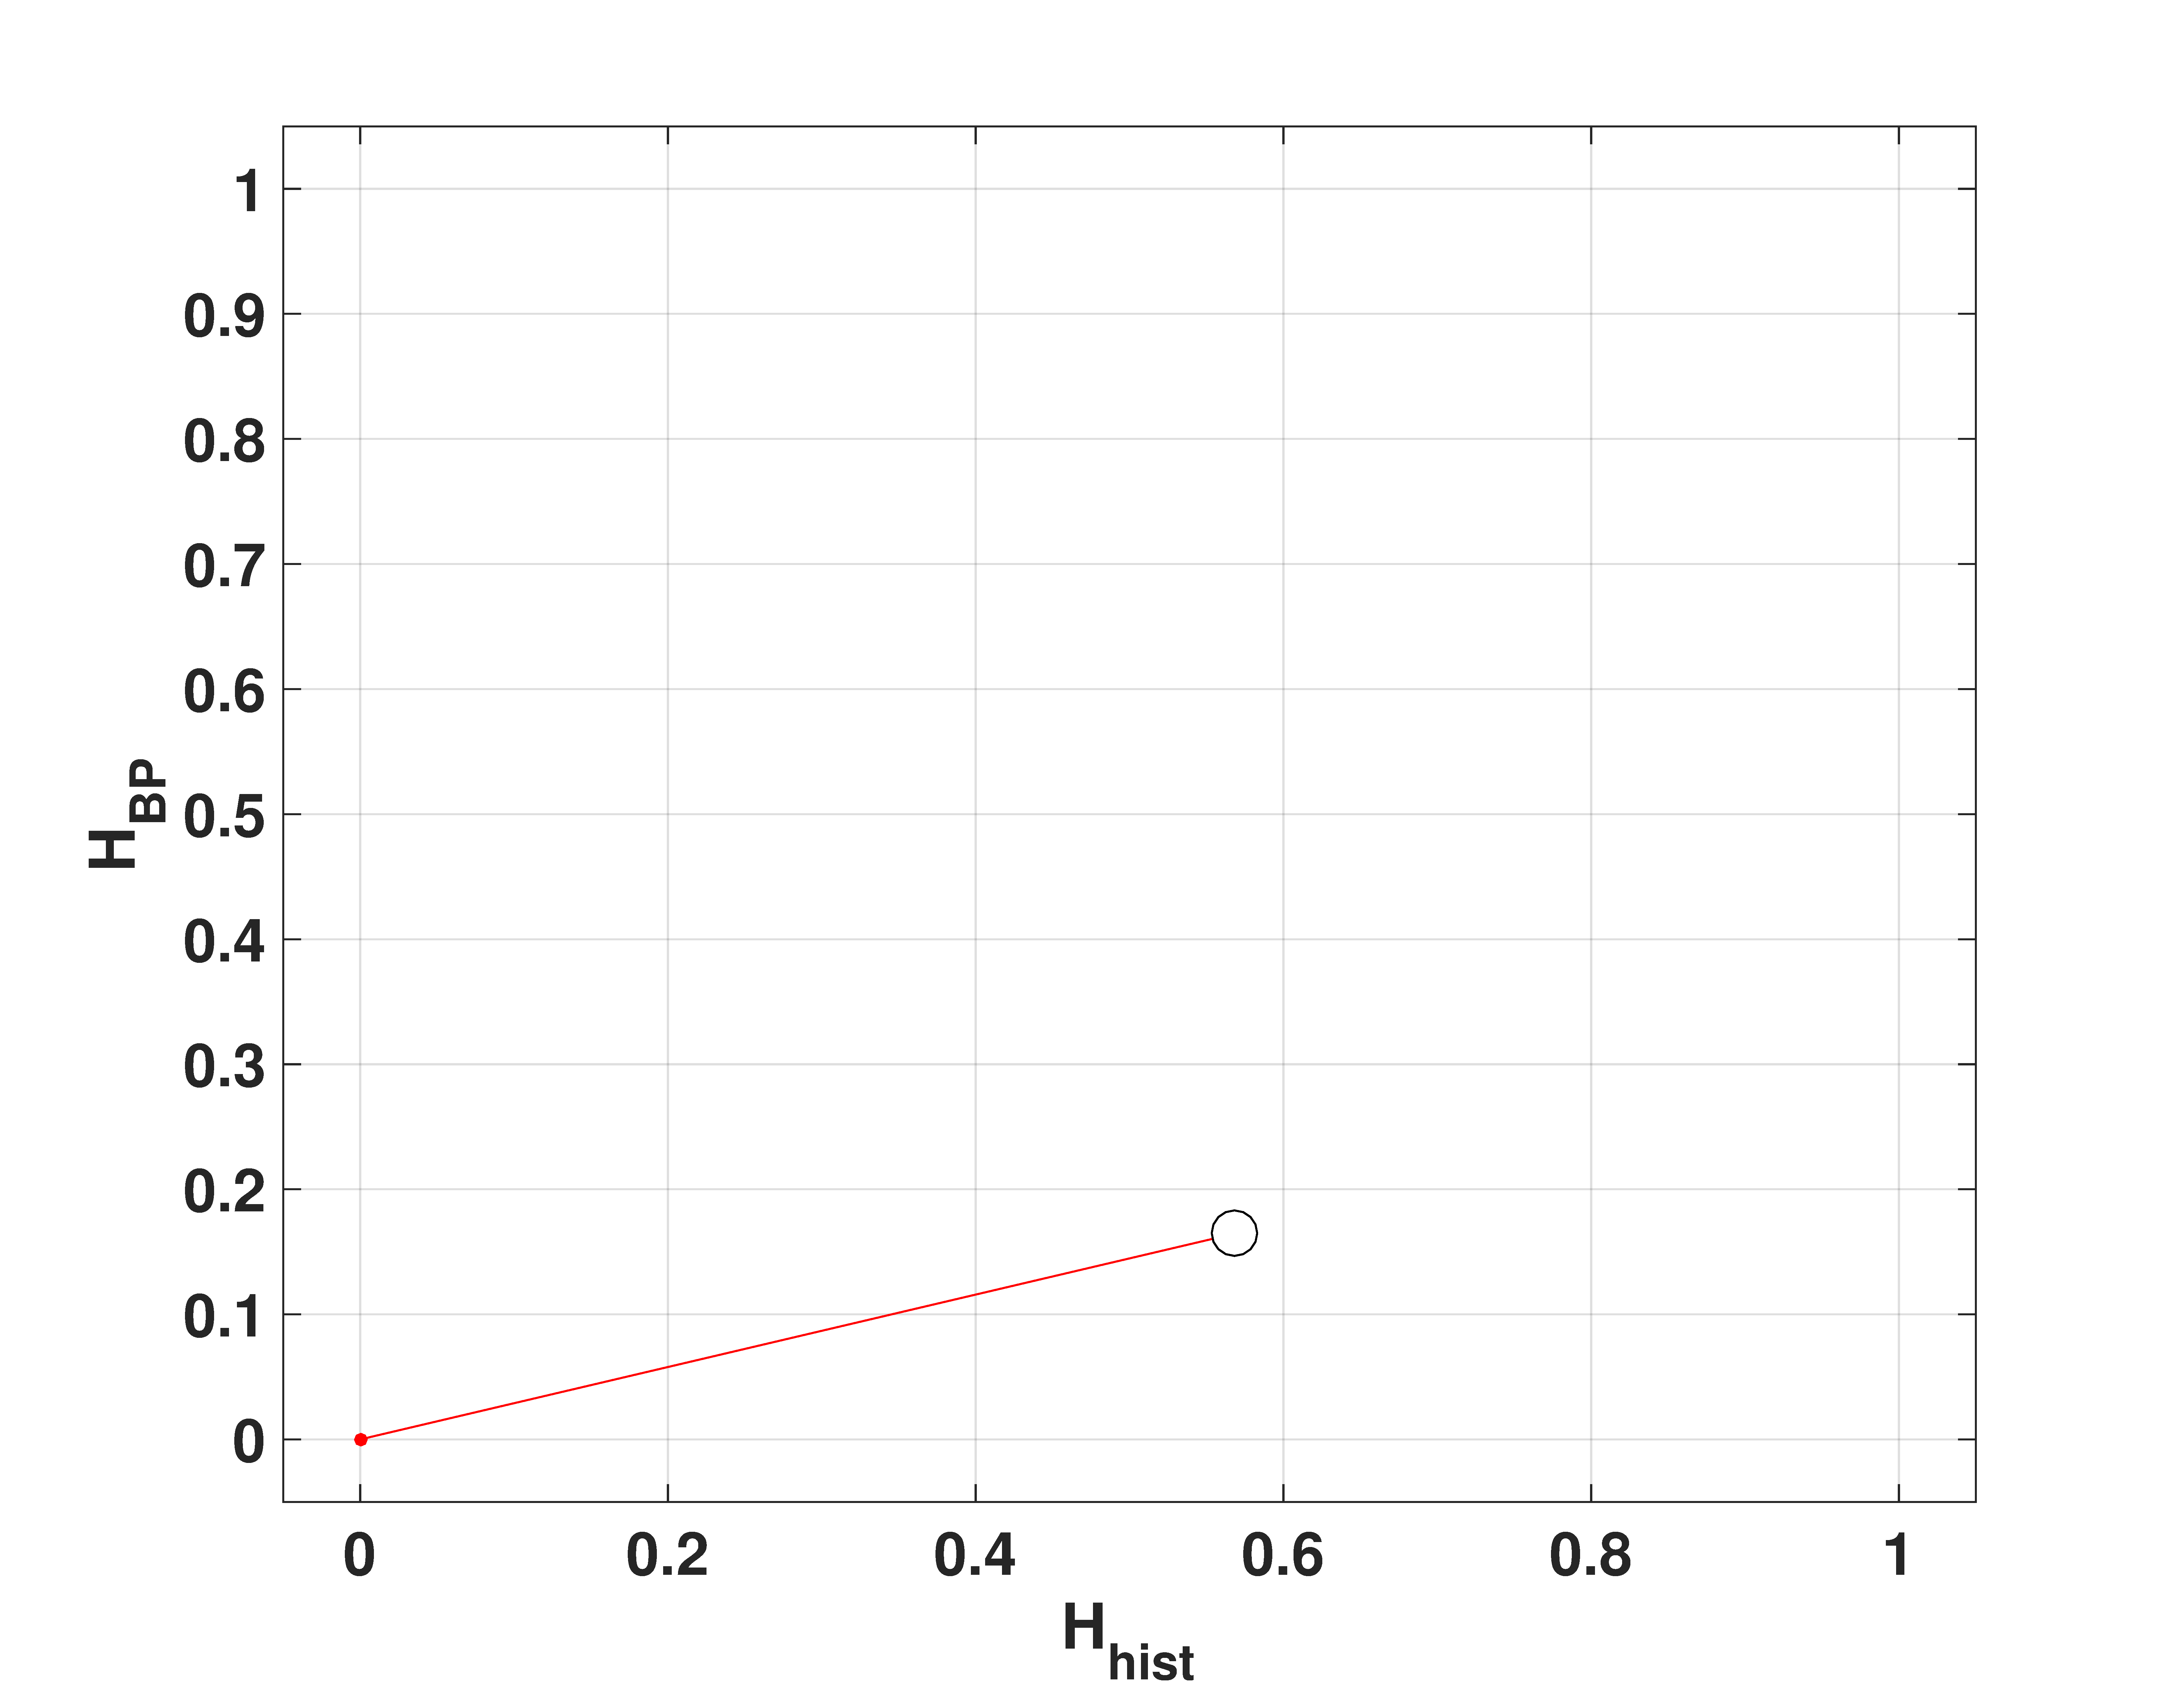
\includegraphics[width=\textwidth]{Senoidal_Hbp_Hhist}
        \caption{Plano deoble entropía}
        \label{subfig:Senoidal_HbpHhist}
    \end{subfigure}
    \caption{Cuantificadores calculados sobre la salida del filtro ideal cuando se ingresa con una senoidal limpia.}\label{fig:Senoidal}
\end{figure}

La salida de los cuantificadores cuando esta señal es contaminada con ruido gaussiano aditivo con $\sigma=0,2$ puede verse en la figura \ref{fig:SenoidalRuidosa}. Vemos en la figura \ref{subfig:SenoidalRuidosa_Hhist} que la entropía de valores aumenta cuando el filtrado no elimina la componente espectral, dando valores incluso sobre el valor de la entropía de la gaussiana. Esto se debe a que la PDF de la senoidal es complementaria con la de la gaussiana, entonces la PDF de la resultante es más parecida a la del ruido uniforme.
Para los patrones de orden de la figura \ref{subfig:SenoidalRuidosa_Hbp}, el pasa-altos no deja ver un cambio significativo debido a que la componente espectral de la senoidal es eliminada en la zona en la que su entropía es alta.
El pasa-bajos en cambio muestra que mientras esta componente está presente el valor de la entropía es asintótico a $H_{BP}\to0,16$ a medida que la frecuencia de corte baja. Recordemos que $H_{BP}\approx0,16$ es el valor de la entropía de patrones de orden de la senoidal limpia.
En el plano doble entropía (figura \ref{subfig:SenoidalRuidosa_HbpHhist}) se ve que ambos cuantificadores son complementarios, en el sentido que la entropía de valores detecta la presencia o no de la señal determinística mientras que la entropía de patrones de orden detecta el filtrado sobre la señal de ruido.
%
\begin{figure}[h]
    \centering
    \begin{subfigure}[t]{0.32\textwidth}
        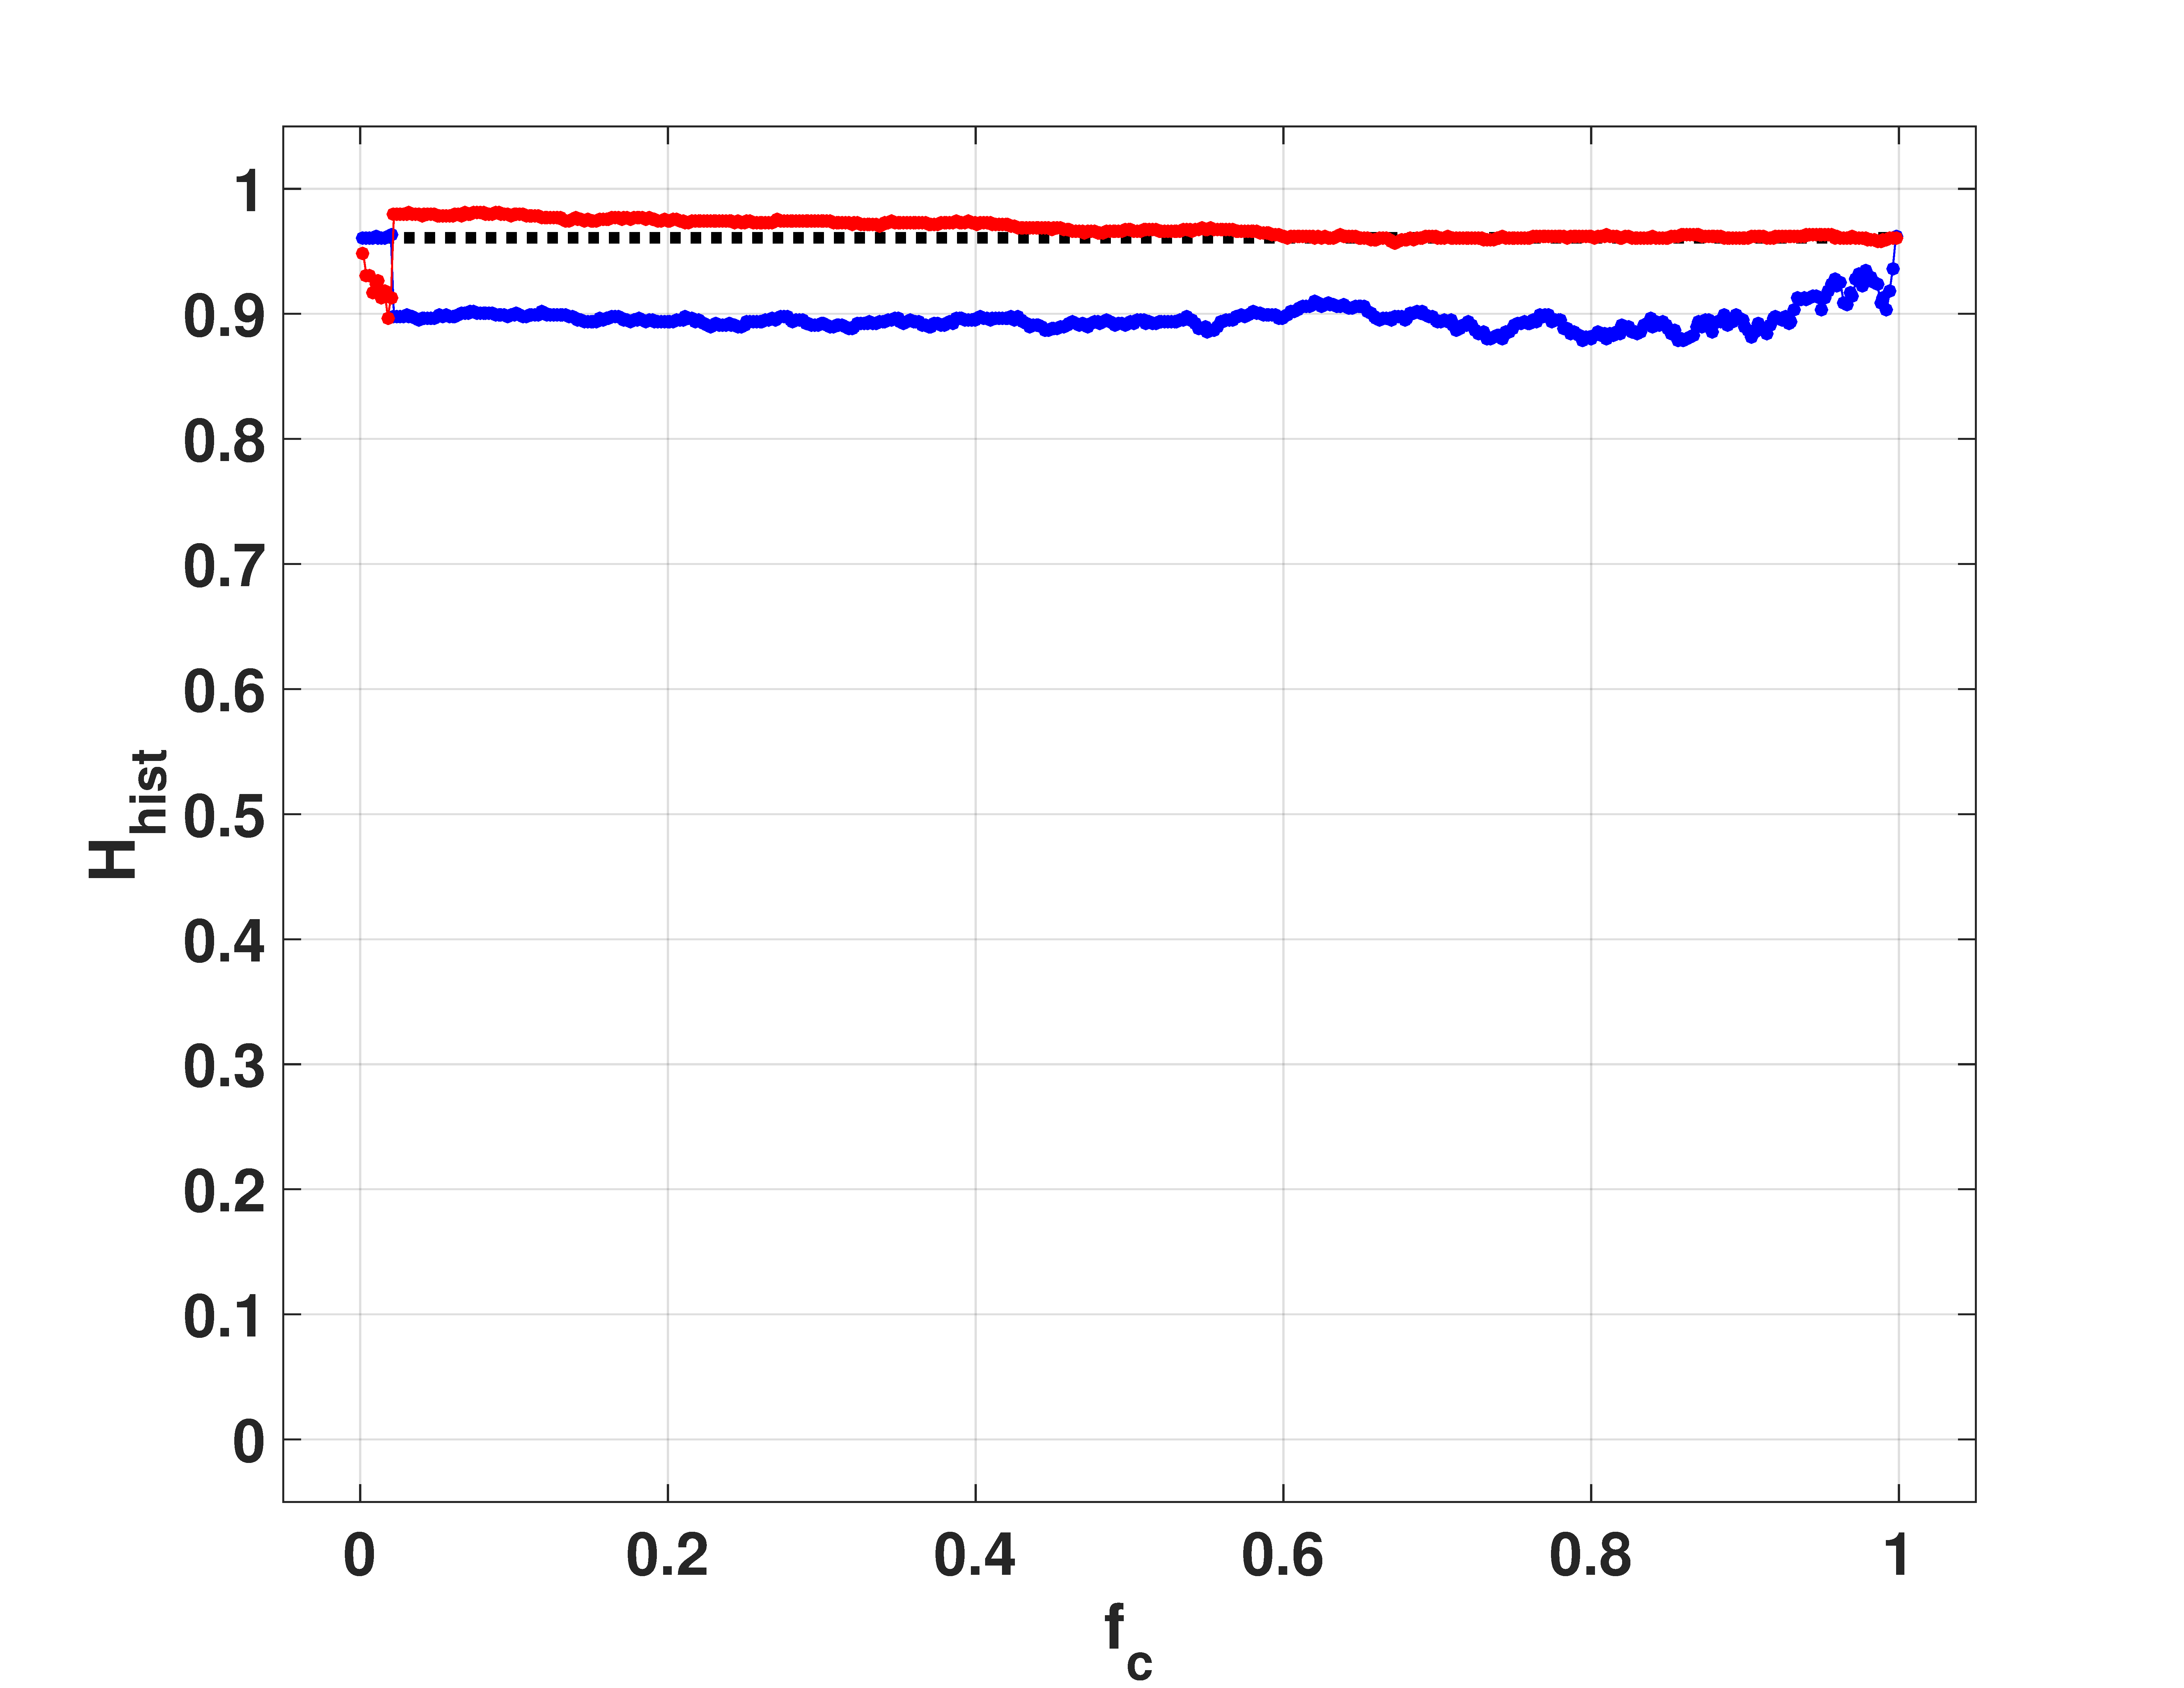
\includegraphics[width=\textwidth]{SenoidalRuidosa_Hhist}
        \caption{Entropía de valores normalizada}
        \label{subfig:SenoidalRuidosa_Hhist}
    \end{subfigure}
    ~ %add desired spacing between images, e. g. ~, \quad, \qquad, \hfill etc. 
      %(or a blank line to force the subfigure onto a new line)
    \begin{subfigure}[t]{0.32\textwidth}
        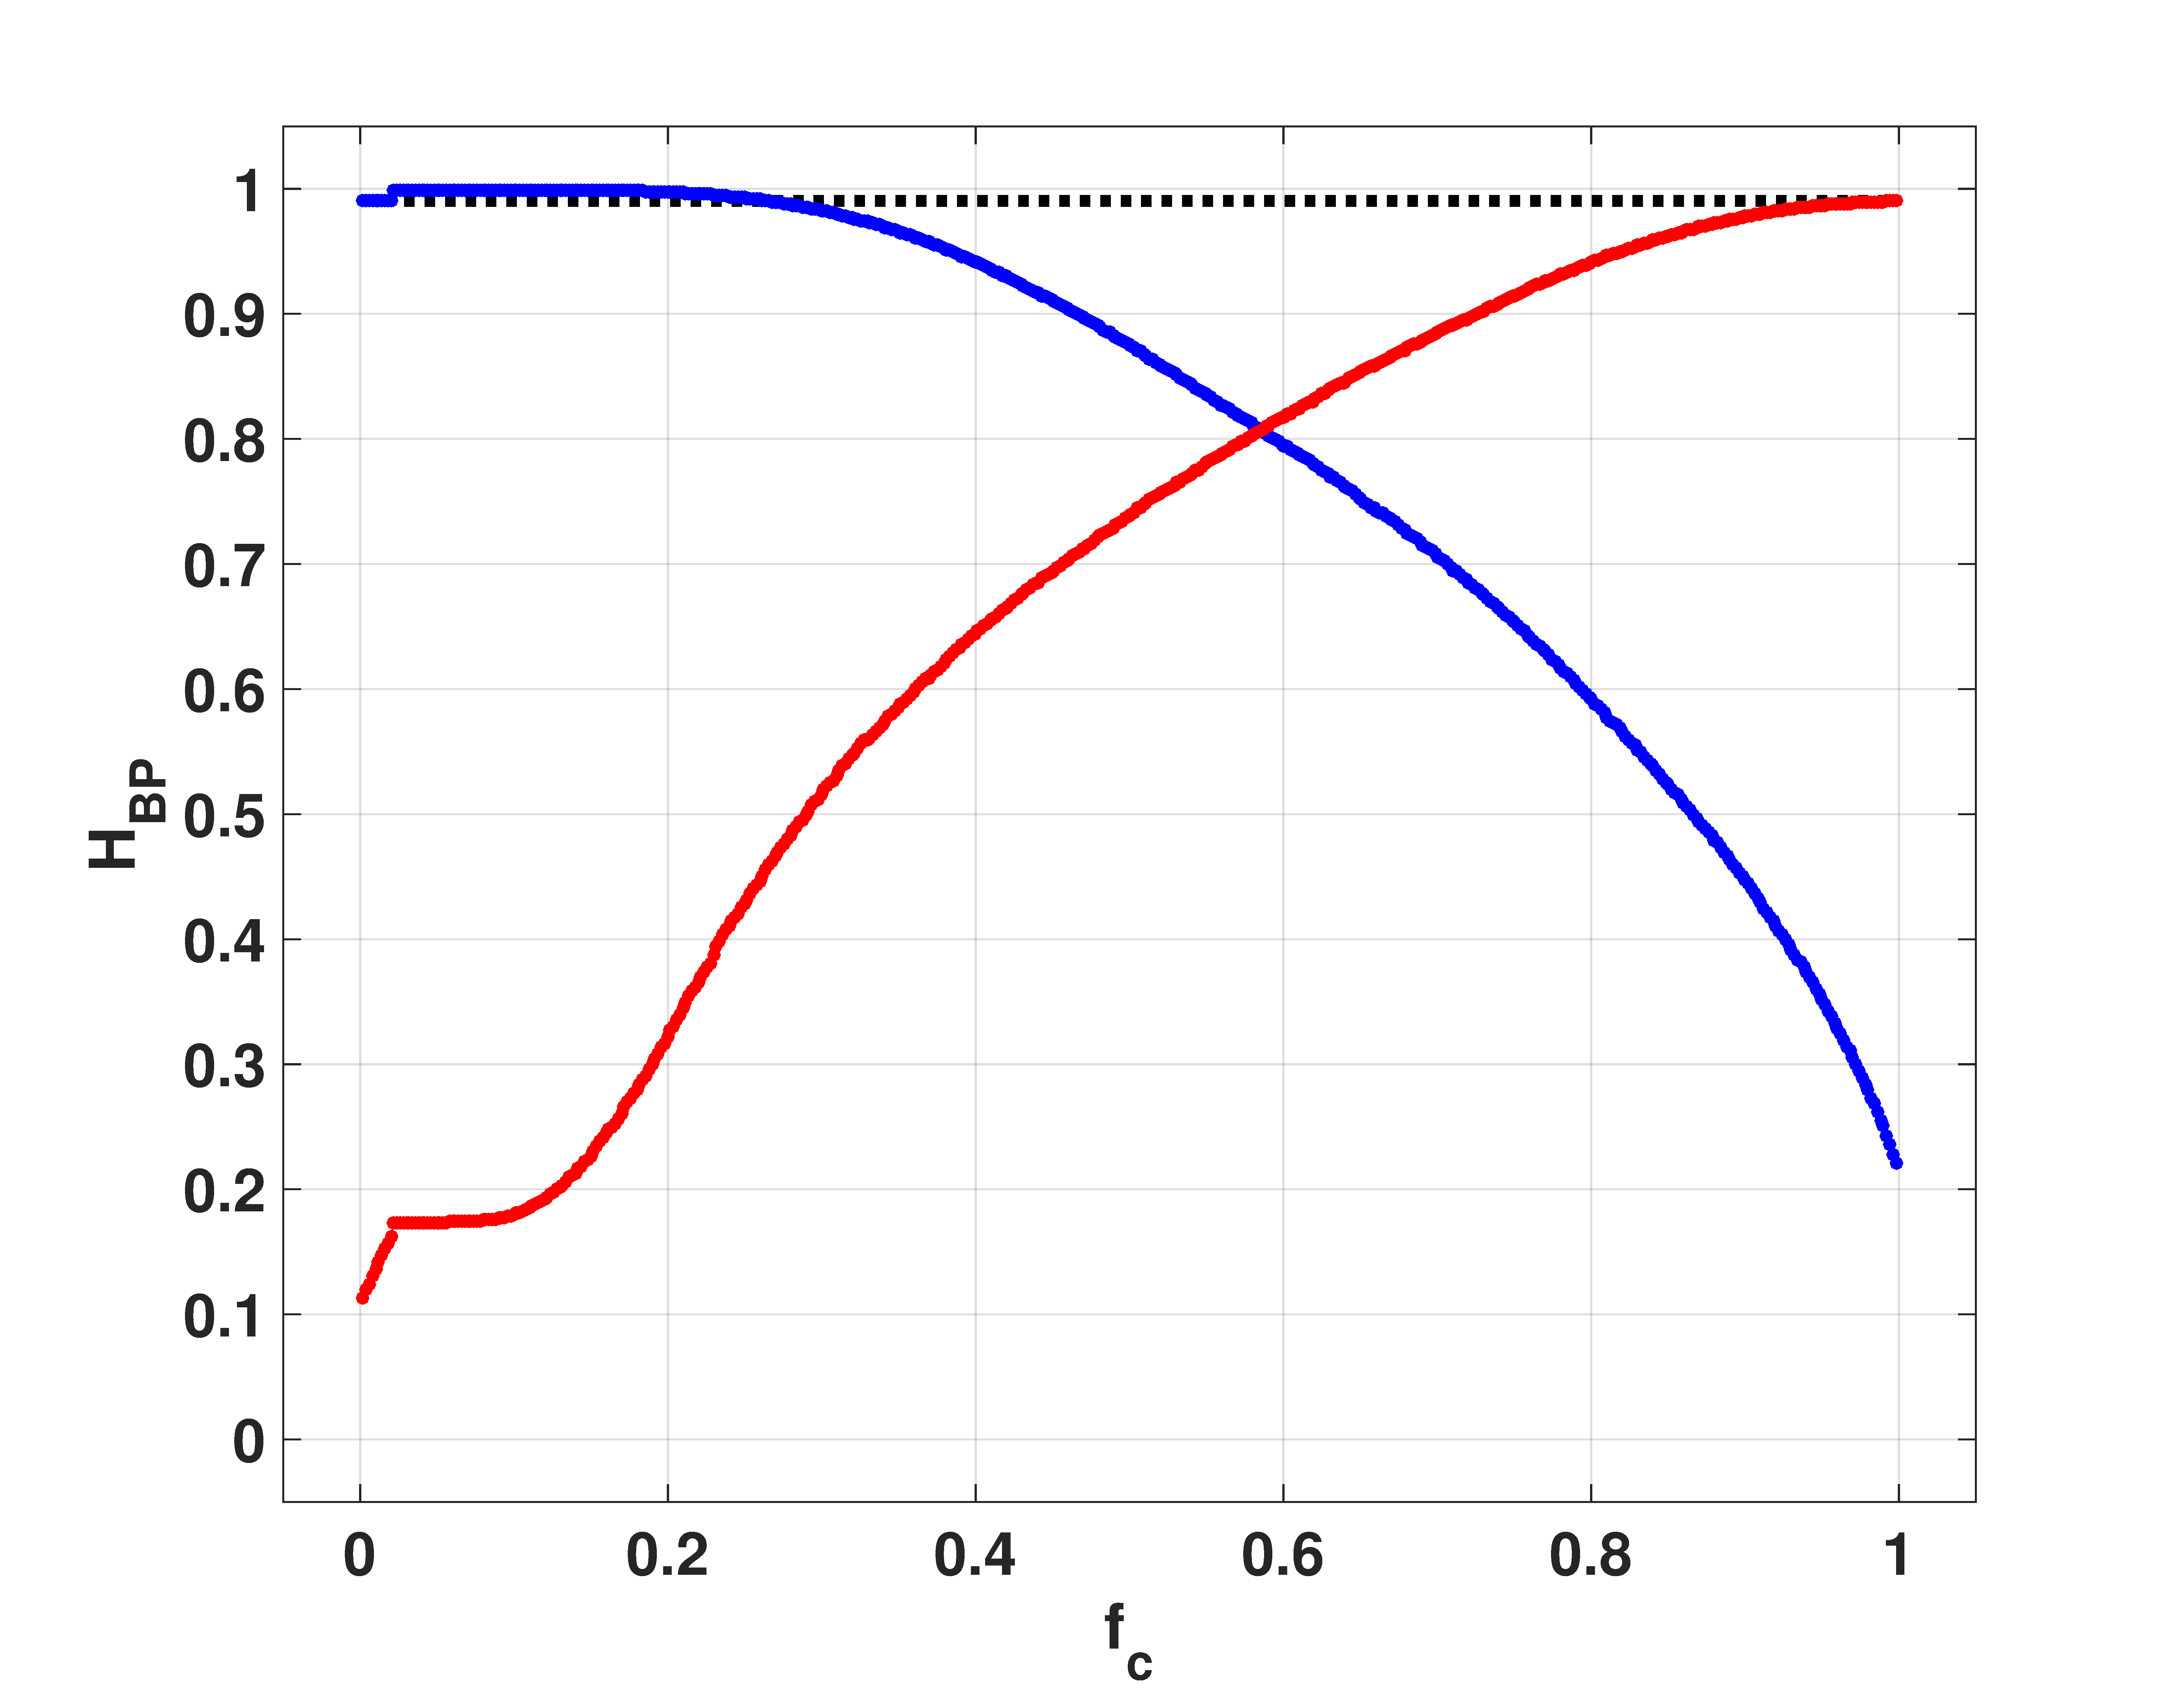
\includegraphics[width=\textwidth]{SenoidalRuidosa_Hbp}
        \caption{Entropía de patrones de orden normalizada}
        \label{subfig:SenoidalRuidosa_Hbp}
    \end{subfigure}
    ~ %add desired spacing between images, e. g. ~, \quad, \qquad, \hfill etc. 
    %(or a blank line to force the subfigure onto a new line)
    \begin{subfigure}[t]{0.32\textwidth}
        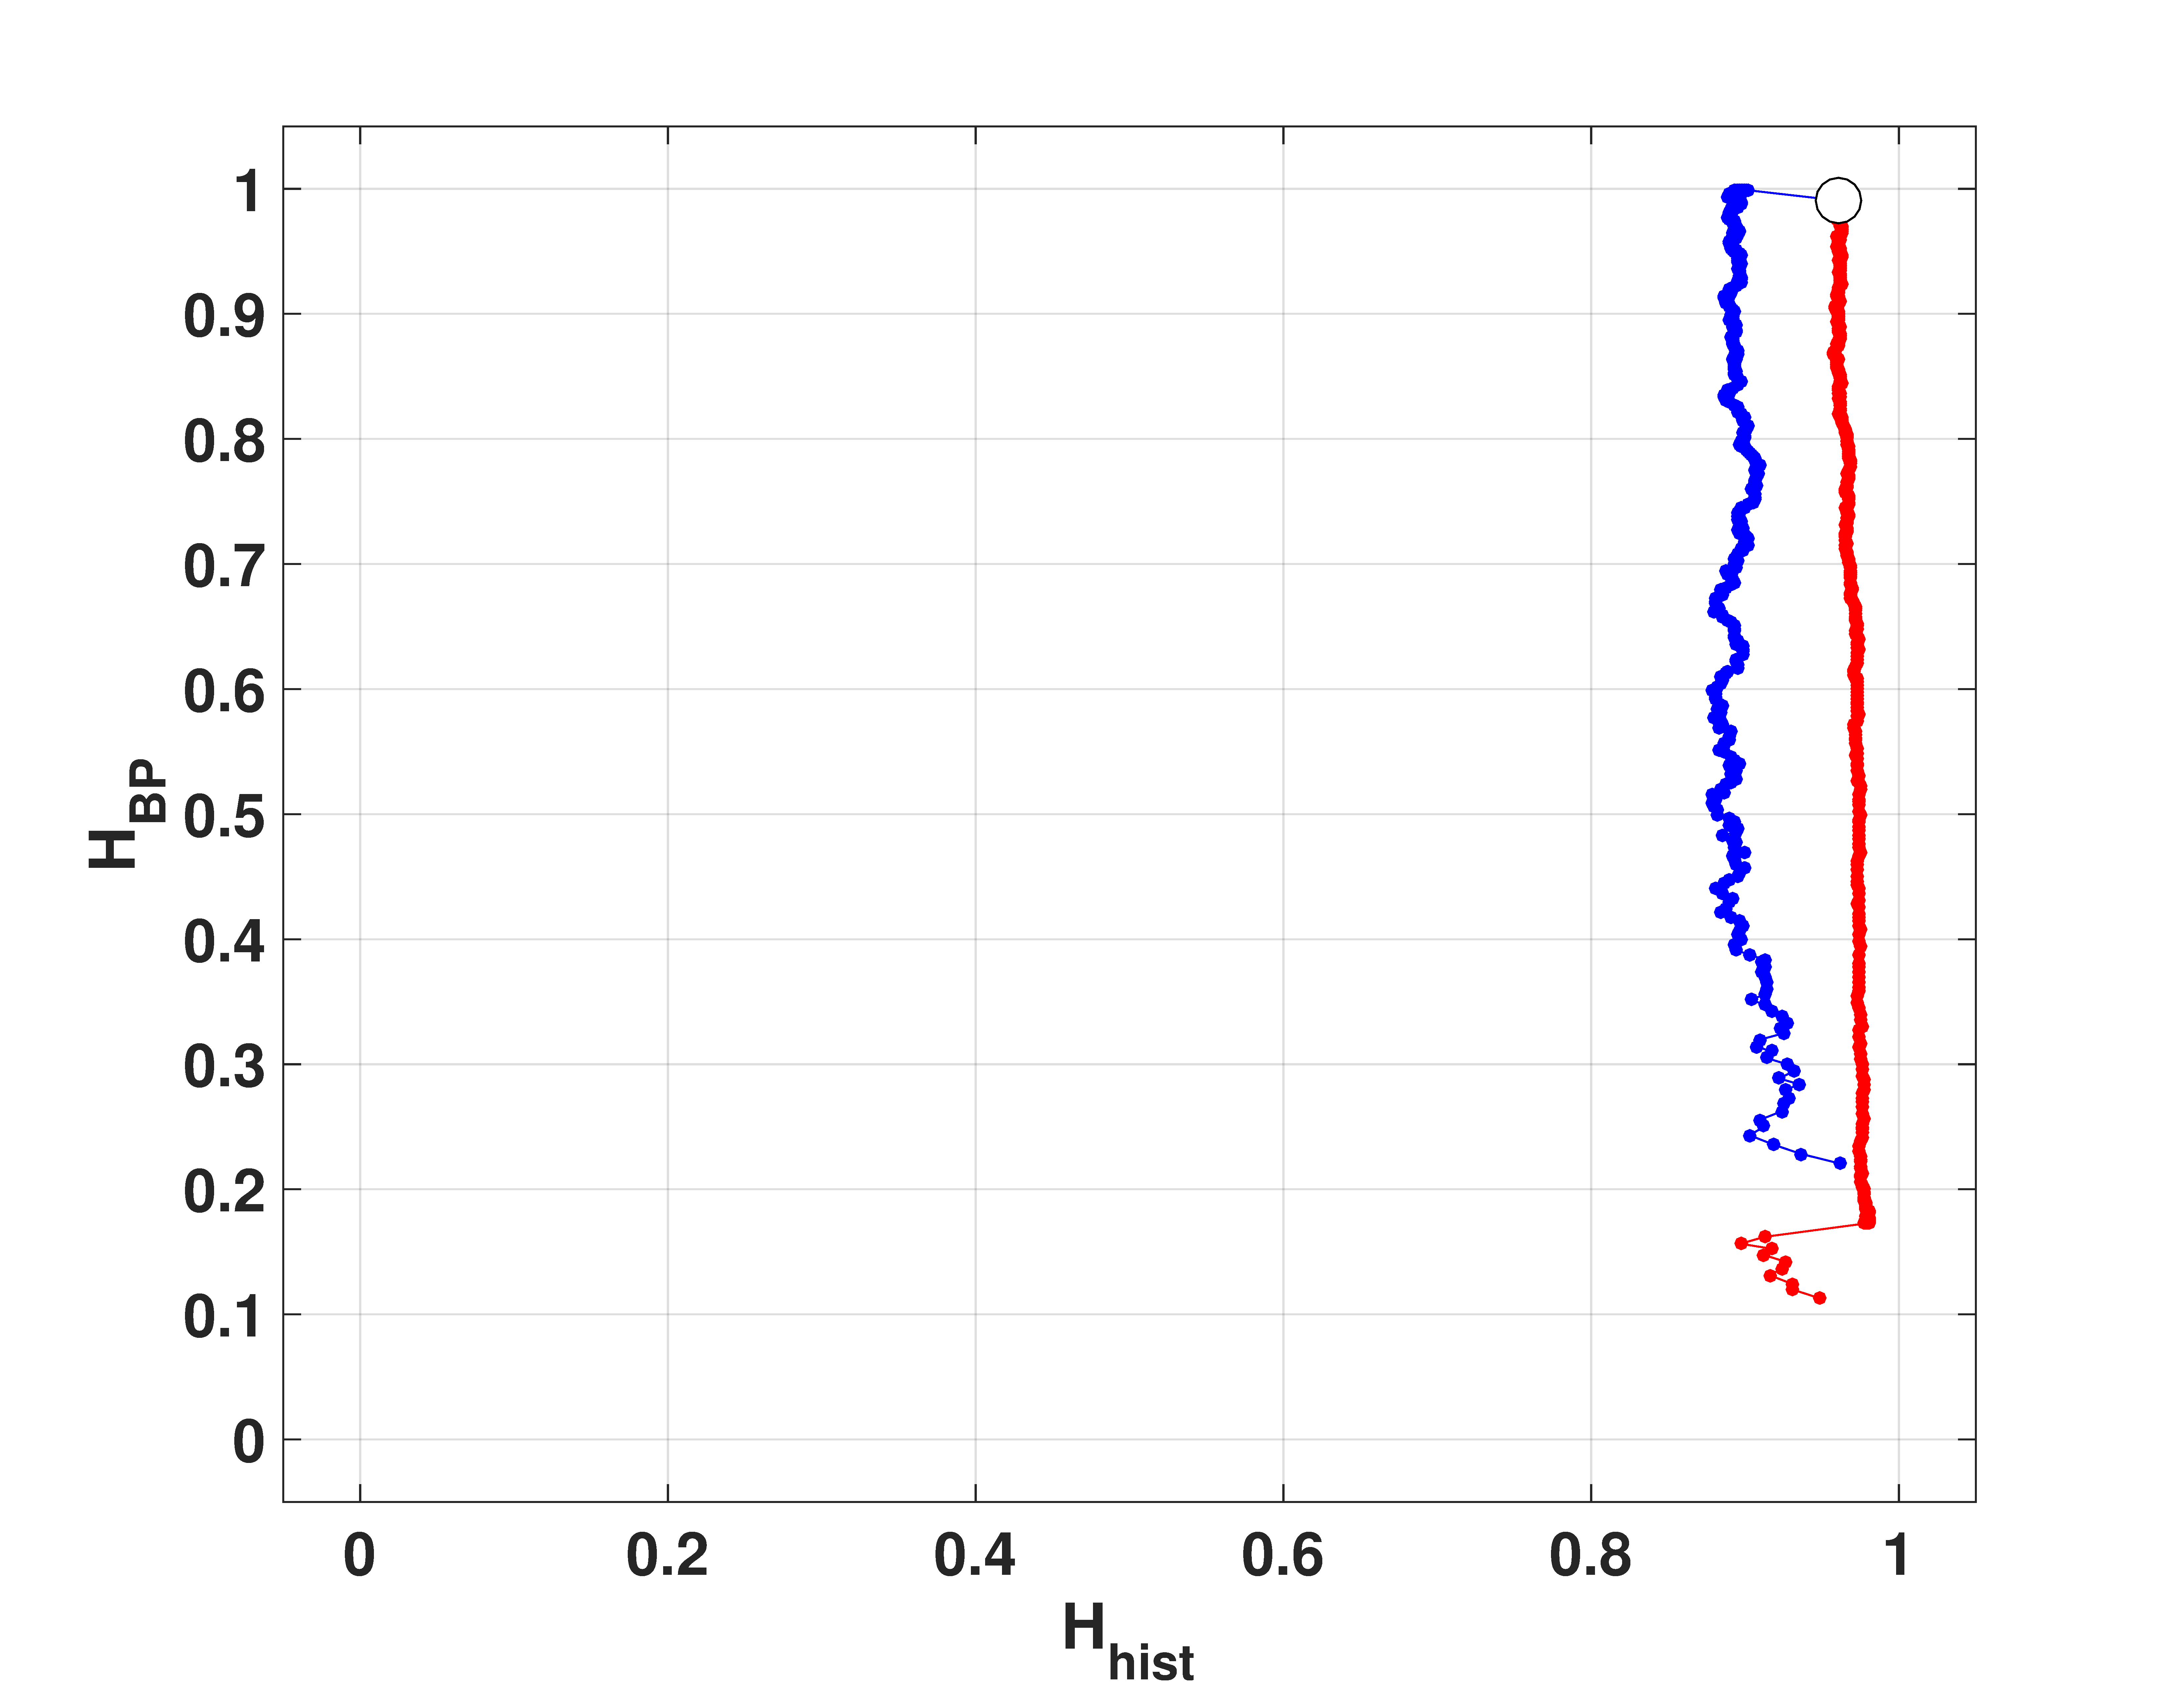
\includegraphics[width=\textwidth]{SenoidalRuidosa_Hbp_Hhist}
        \caption{Plano deoble entropía}
        \label{subfig:SenoidalRuidosa_HbpHhist}
    \end{subfigure}
    \caption{Cuantificadores calculados sobre la salida del filtro ideal cuando se ingresa con una senoidal ruidosa.}\label{fig:SenoidalRuidosa}
\end{figure}

En la figura \ref{fig:Cuadrada} se muestran los resultados cuando la señal determinística es una cuadrada sin ruido de amplitud unitaria y período de $100$ muestras. Tanto la entropía de valores $H_{hist}$ como la entropía de patrones de orden $H_{BP}$ presentan una forma escalonada, sus valores se mantienen constantes a medida que se barre la frecuencia de corte de los filtros hasta que la siguiente componente espectral es filtrada. También se ve que en ambos casos los valores resultantes se mantienen bastante lejos del valor sin filtrar, que se muestra con una linea negra punteada.
%
\begin{figure}[h]
    \centering
    \begin{subfigure}[t]{0.32\textwidth}
        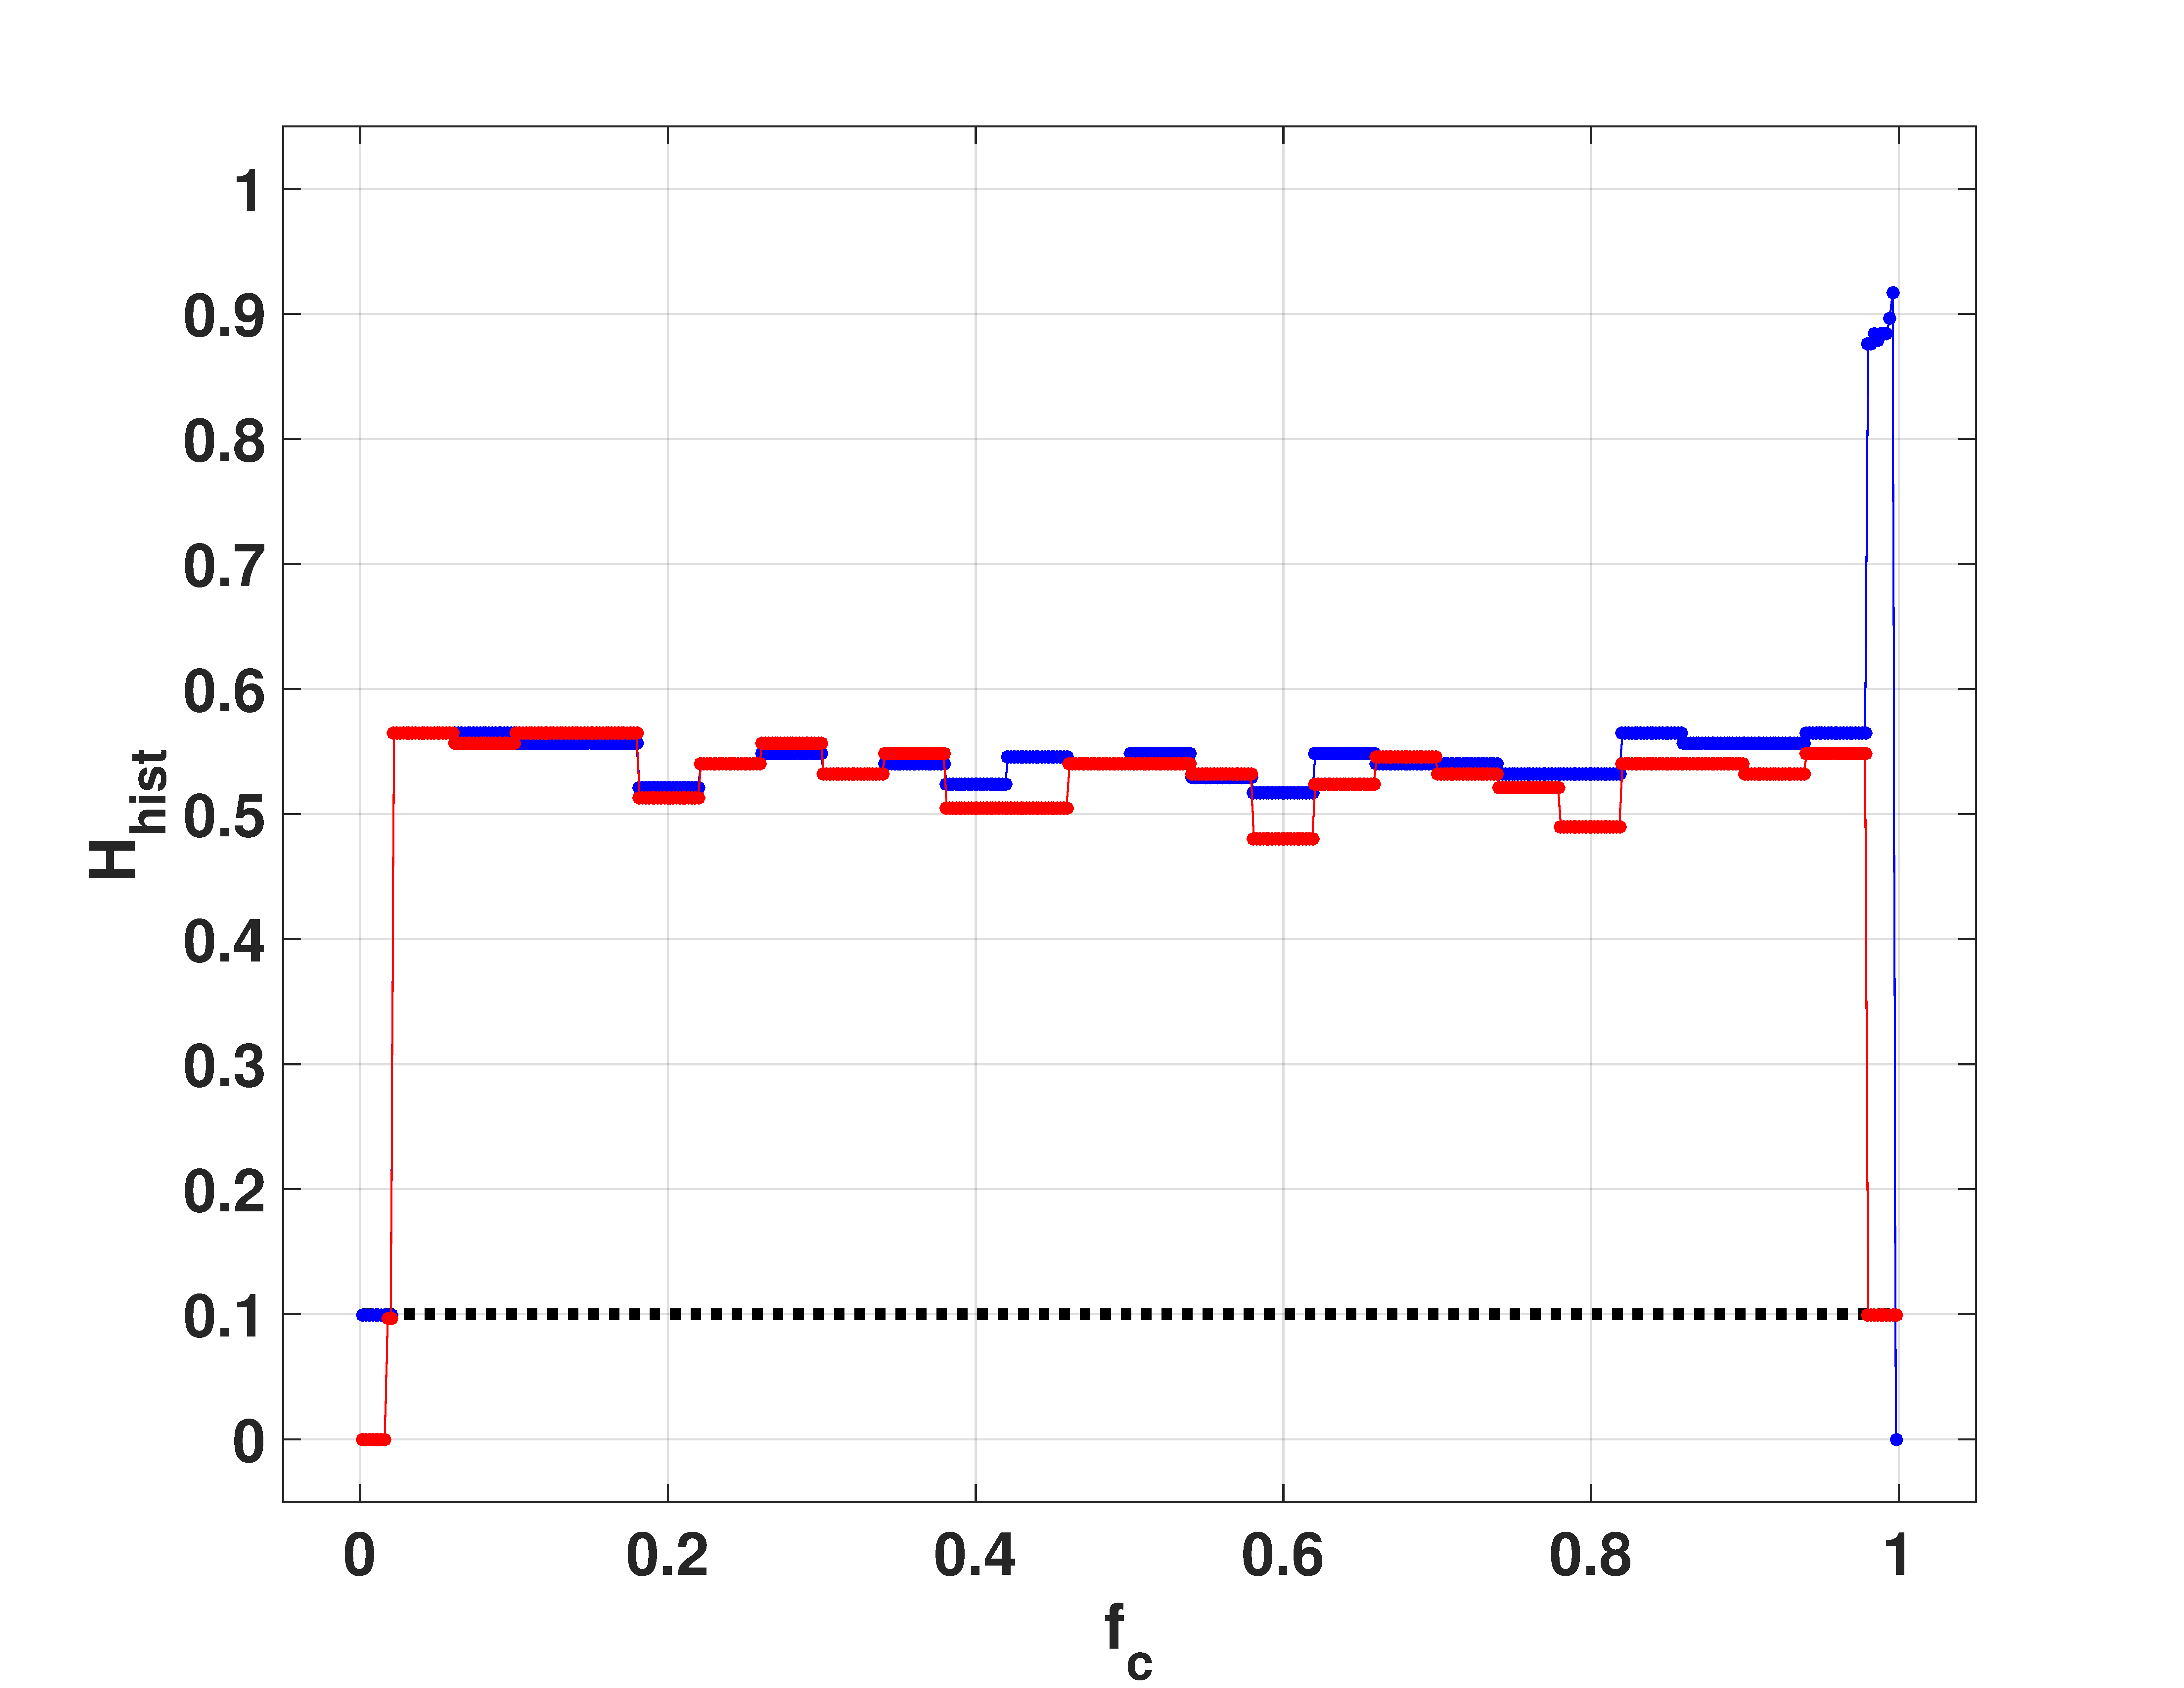
\includegraphics[width=\textwidth]{Cuadrada_Hhist}
        \caption{Entropía de valores normalizada}
        \label{subfig:Cuadrada_Hhist}
    \end{subfigure}
    ~ %add desired spacing between images, e. g. ~, \quad, \qquad, \hfill etc. 
      %(or a blank line to force the subfigure onto a new line)
    \begin{subfigure}[t]{0.32\textwidth}
        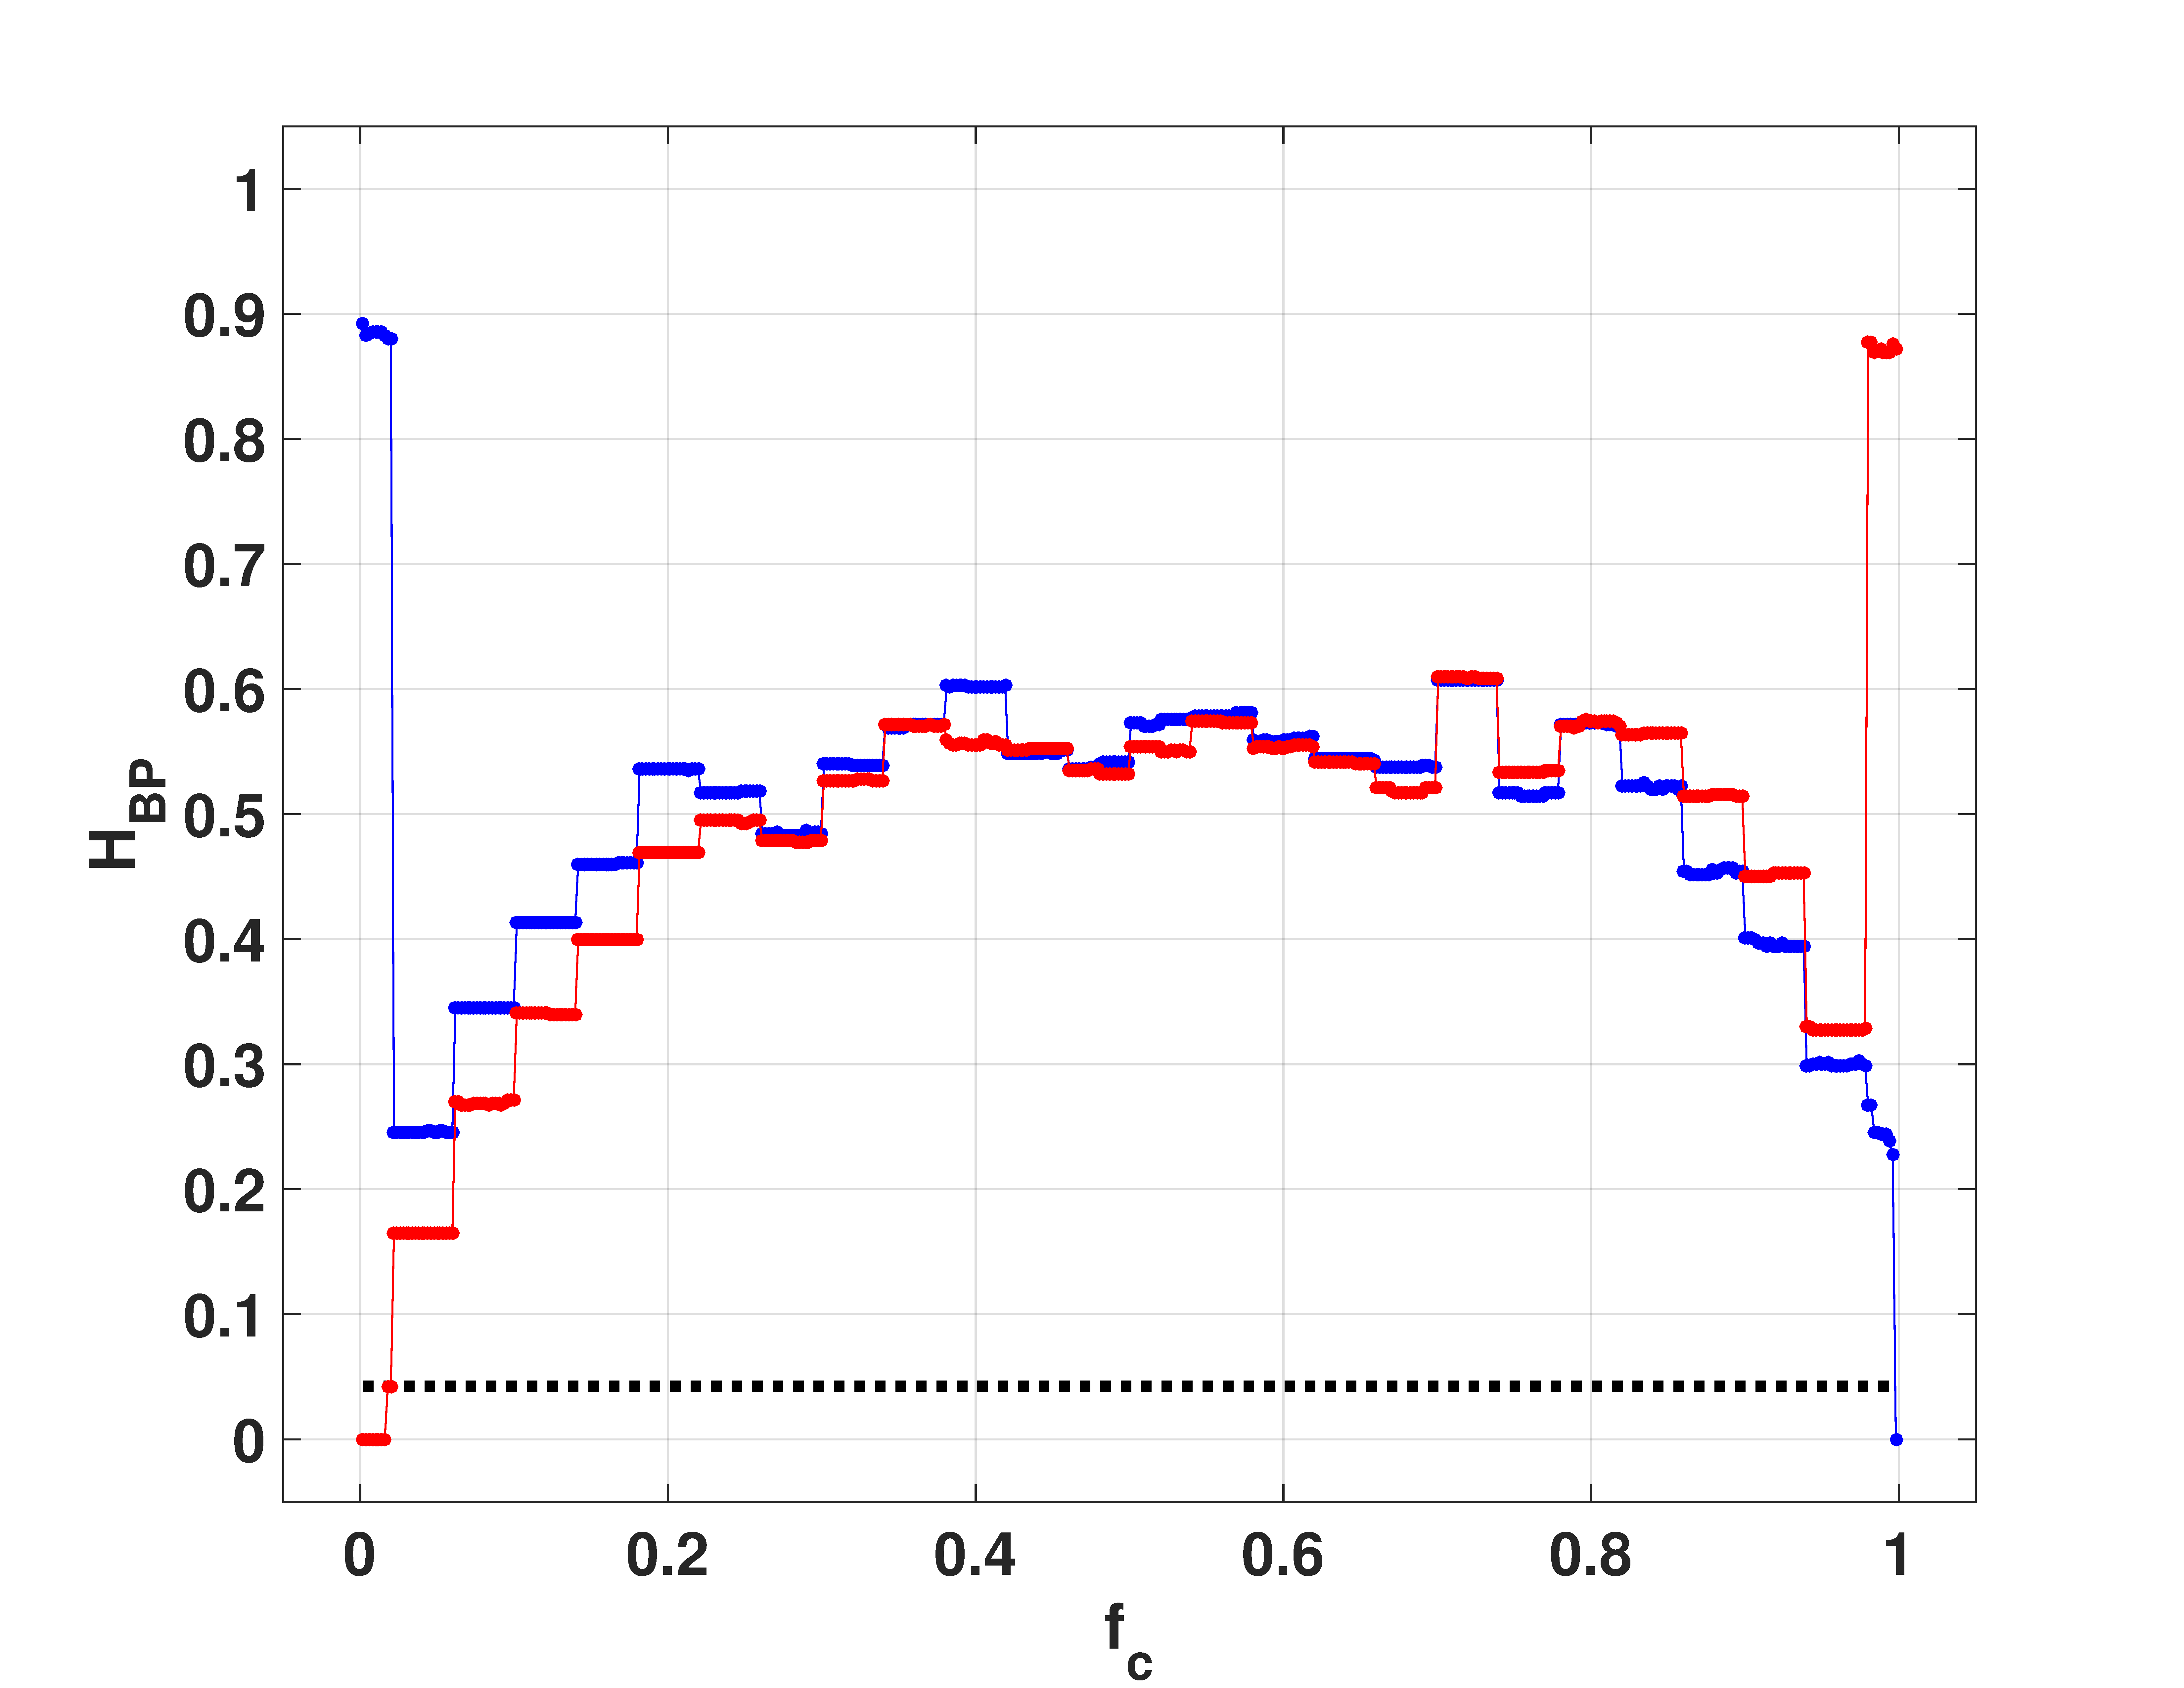
\includegraphics[width=\textwidth]{Cuadrada_Hbp}
        \caption{Entropía de patrones de orden normalizada}
        \label{subfig:Cuadrada_Hbp}
    \end{subfigure}
    ~ %add desired spacing between images, e. g. ~, \quad, \qquad, \hfill etc. 
    %(or a blank line to force the subfigure onto a new line)
    \begin{subfigure}[t]{0.32\textwidth}
        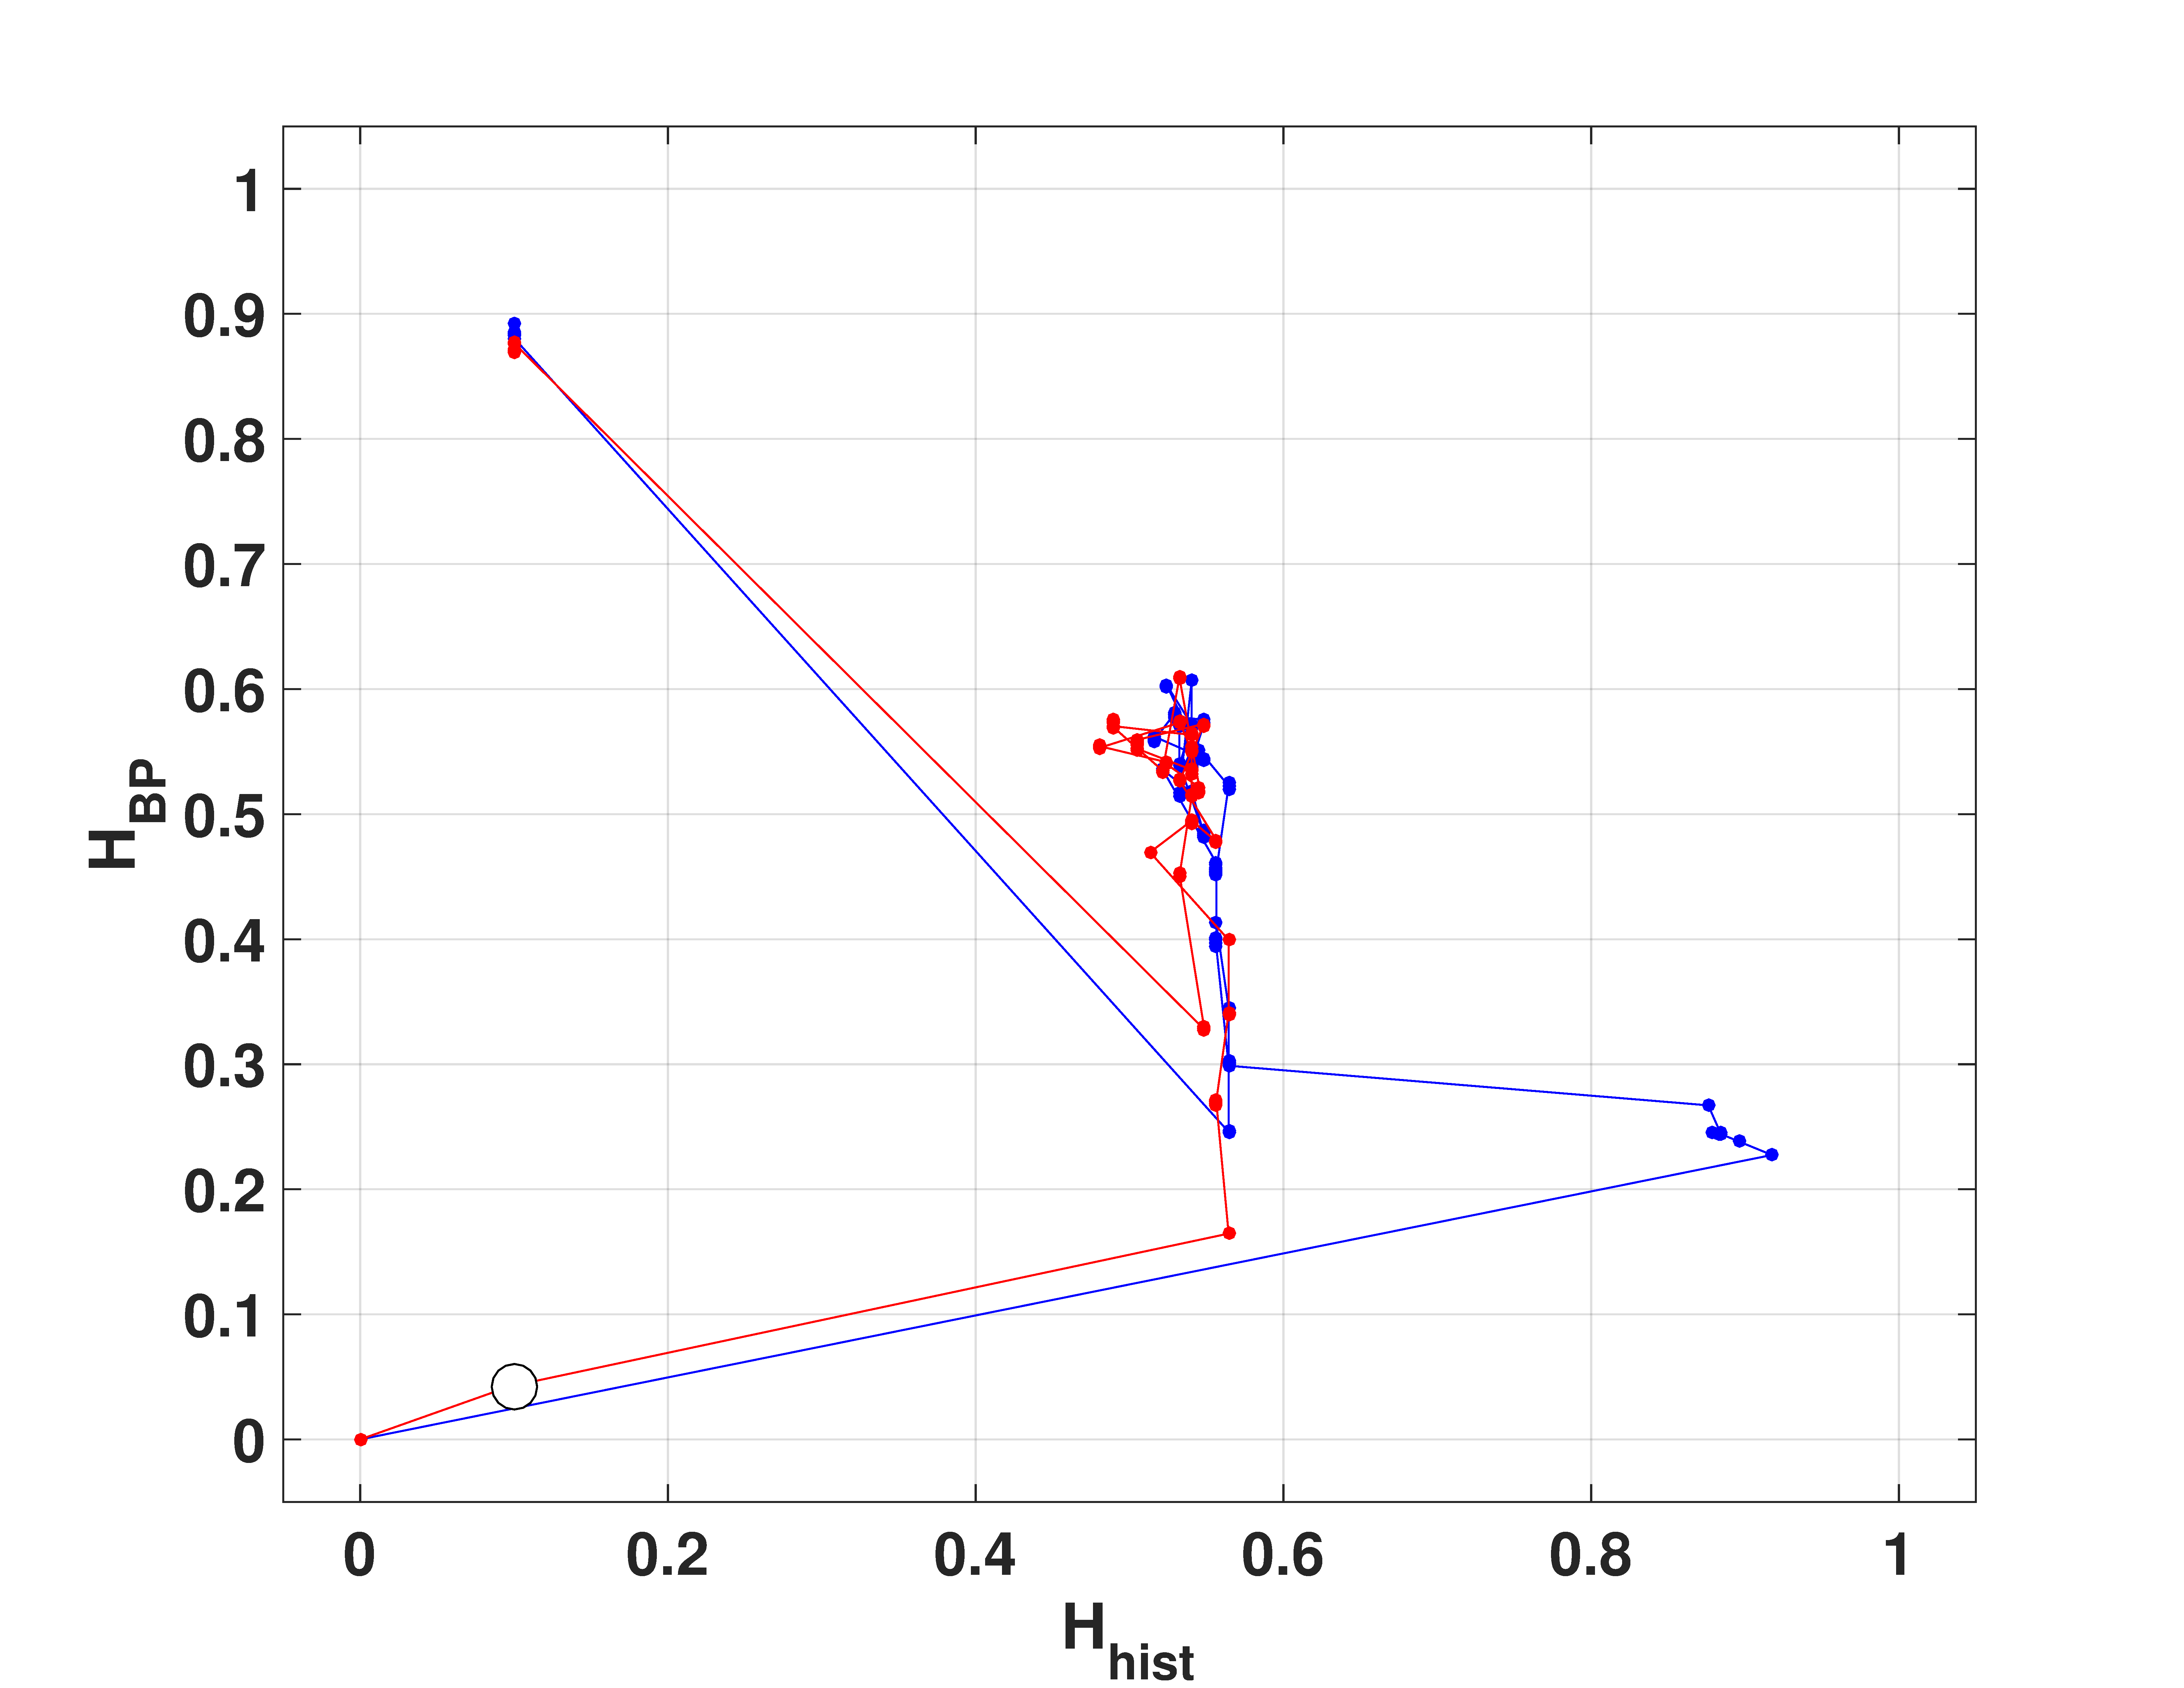
\includegraphics[width=\textwidth]{Cuadrada_Hbp_Hhist}
        \caption{Plano deoble entropía}
        \label{subfig:Cuadrada_HbpHhist}
    \end{subfigure}
    \caption{Cuantificadores calculados sobre la salida del filtro ideal cuando se ingresa con una cuadrada limpia.}\label{fig:Cuadrada}
\end{figure}

El caso contaminado con ruido (figura \ref{fig:CuadradaRuidosa}) cambia respecto del caso sin contaminar. En la figura \ref{subfig:CuadradaRuidosa_Hhist} se ve que para el pasabajos (rojo) $H_{hist}$ se mantiene alrededor del valor sin filtrar (linea punteada), excepto con las tres frecuencias más bajas, en donde su valor aumenta un levemente por las mismas razones que aumentaba con la senoidal contaminada.
Algo parecido sucede con $H_{BP}$ en la figura \ref{subfig:CuadradaRuidosa_Hbp}. Cuando la cuadrada se contamina con ruido su valor se mantiene cercano al del ruido gaussiano, esto es por que en las regiones en las que la cuadrada es plana su contribución al patrón de orden es nula. Para el pasa bajos se ve un escalonado en la posición de cada componente espectral que se hace más notorio para las frecuencias más bajas, en donde la contribución del ruido ya es bastante baja y a la vez se encuentran las componentes espectrales de mayor peso. Esto no es tan notorio en el pasa-altos, en este caso cuando la contribución del ruido es de baja amplitud también lo es la de la determinística, enmascarando este fenómeno.
%
\begin{figure}[h]
    \centering
    \begin{subfigure}[t]{0.32\textwidth}
        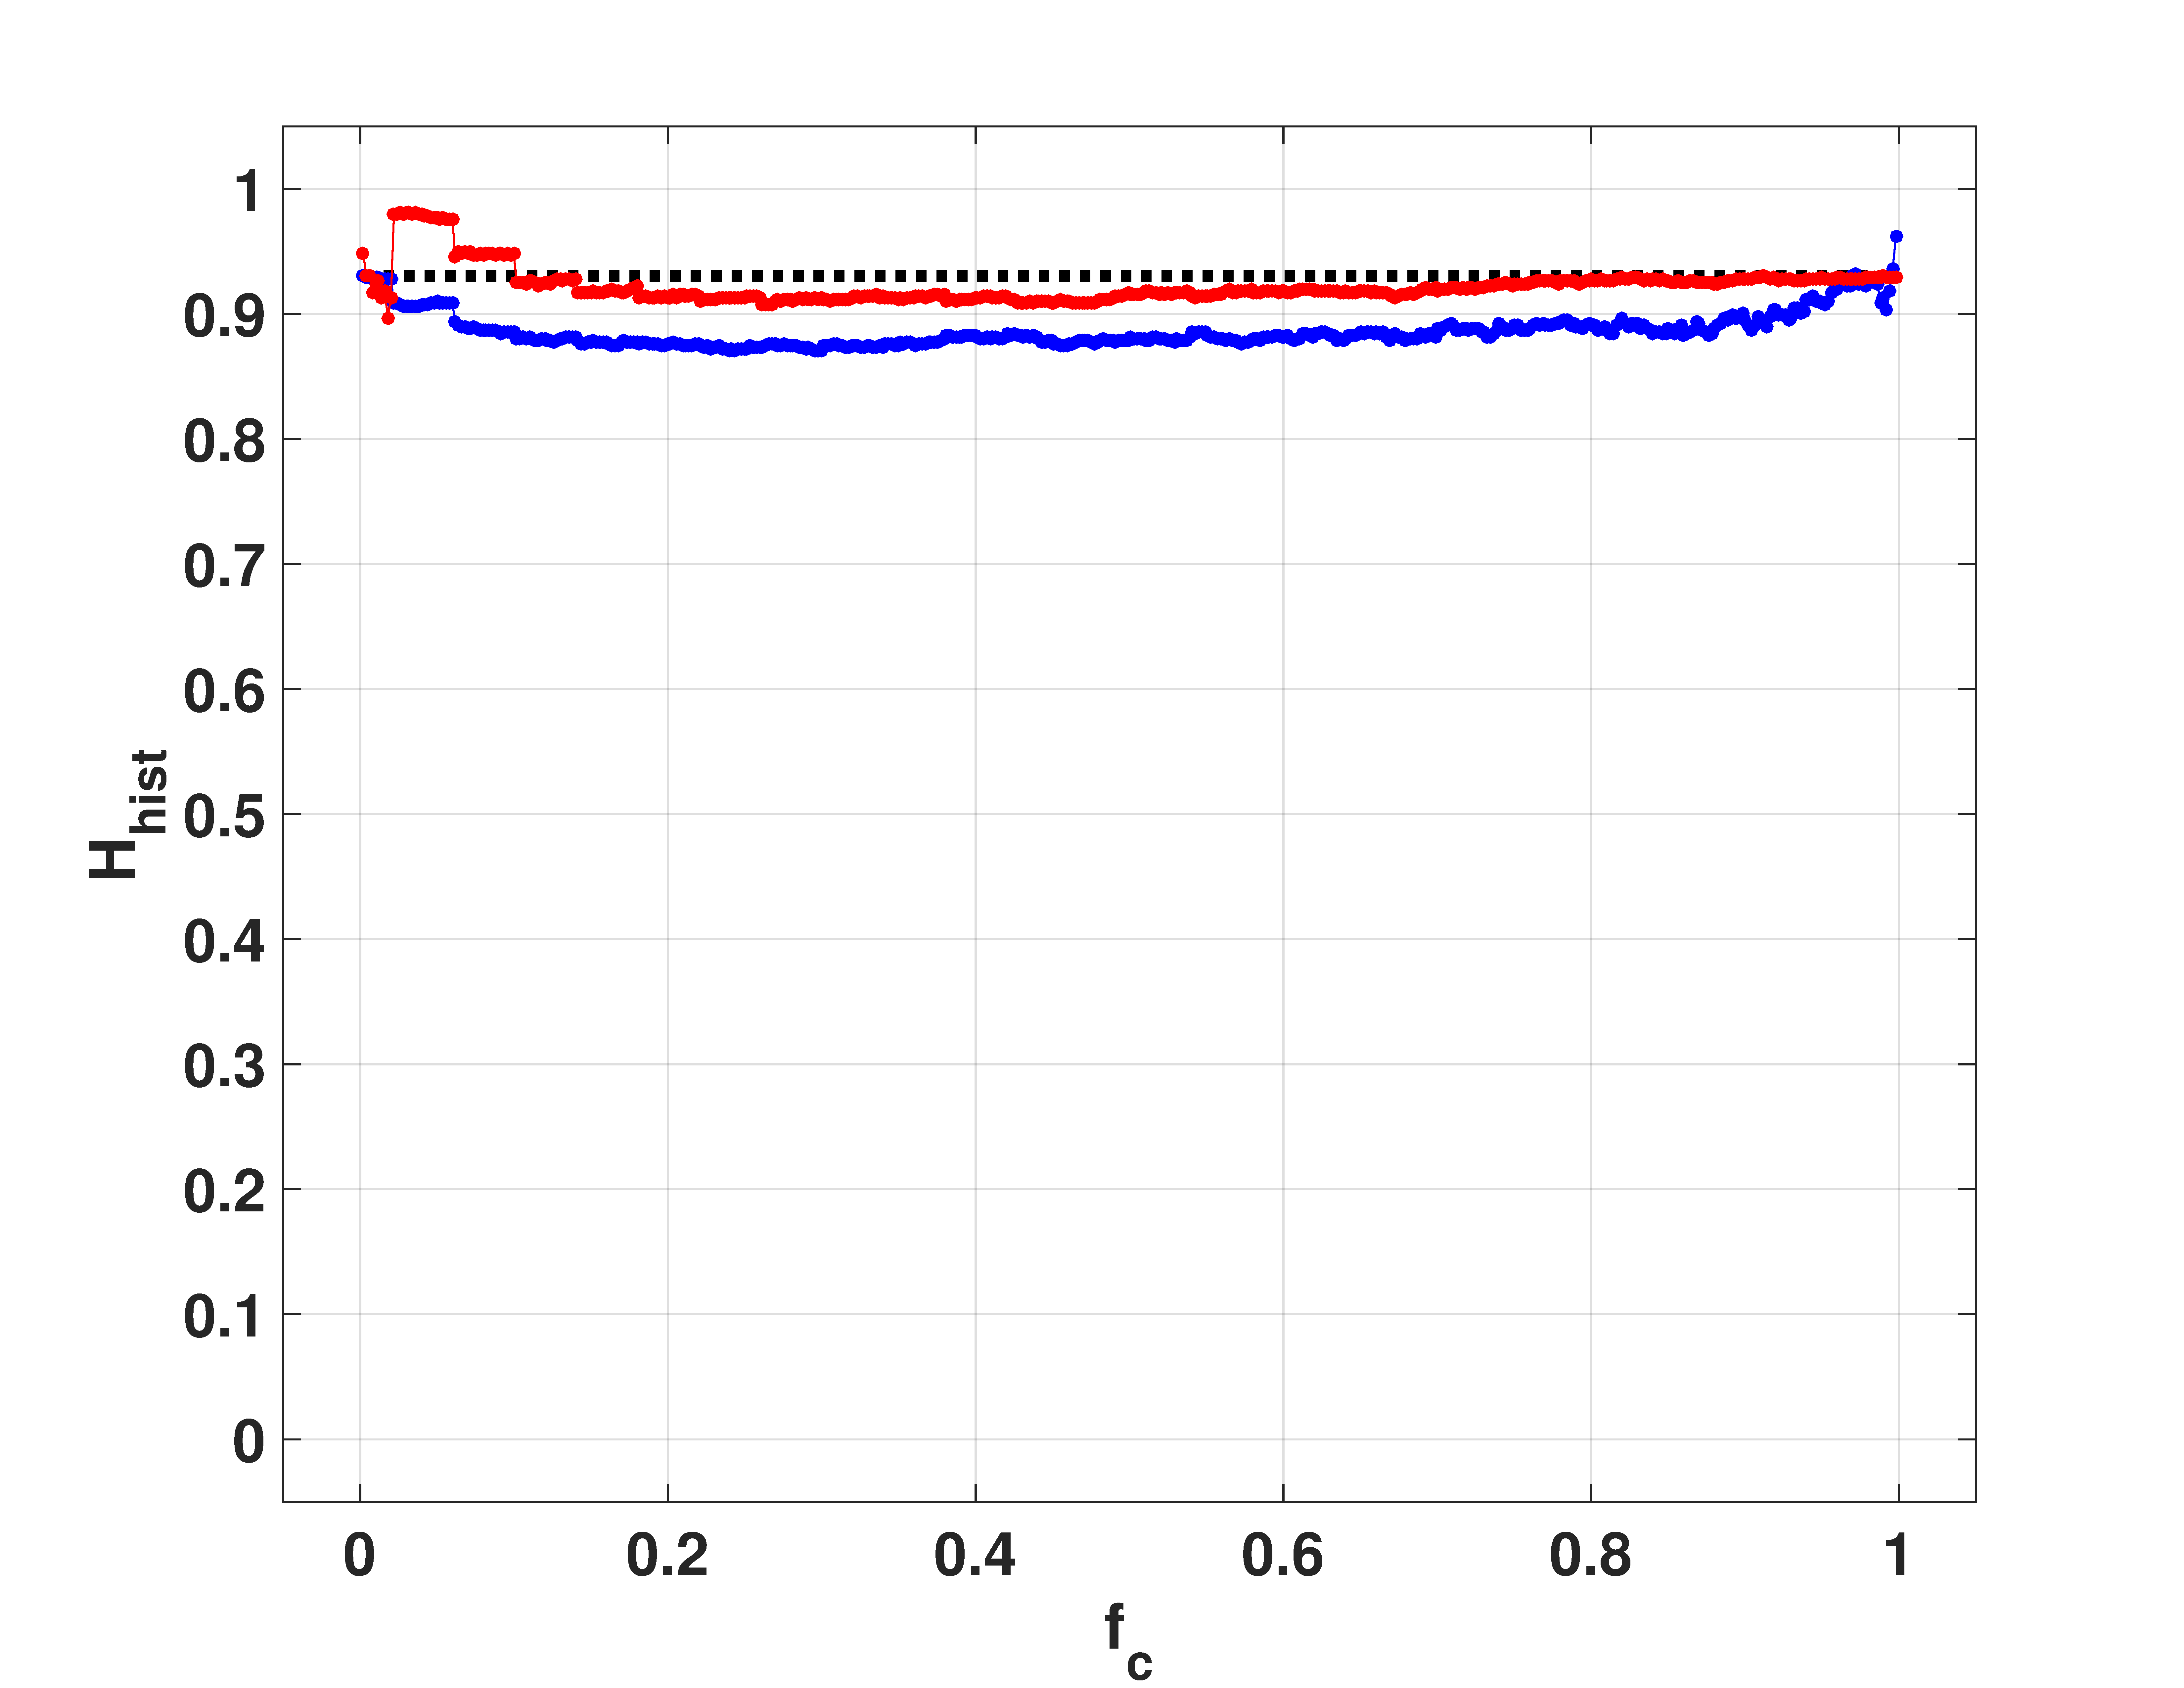
\includegraphics[width=\textwidth]{CuadradaRuidosa_Hhist}
        \caption{Entropía de valores normalizada}
        \label{subfig:CuadradaRuidosa_Hhist}
    \end{subfigure}
    ~ %add desired spacing between images, e. g. ~, \quad, \qquad, \hfill etc. 
      %(or a blank line to force the subfigure onto a new line)
    \begin{subfigure}[t]{0.32\textwidth}
        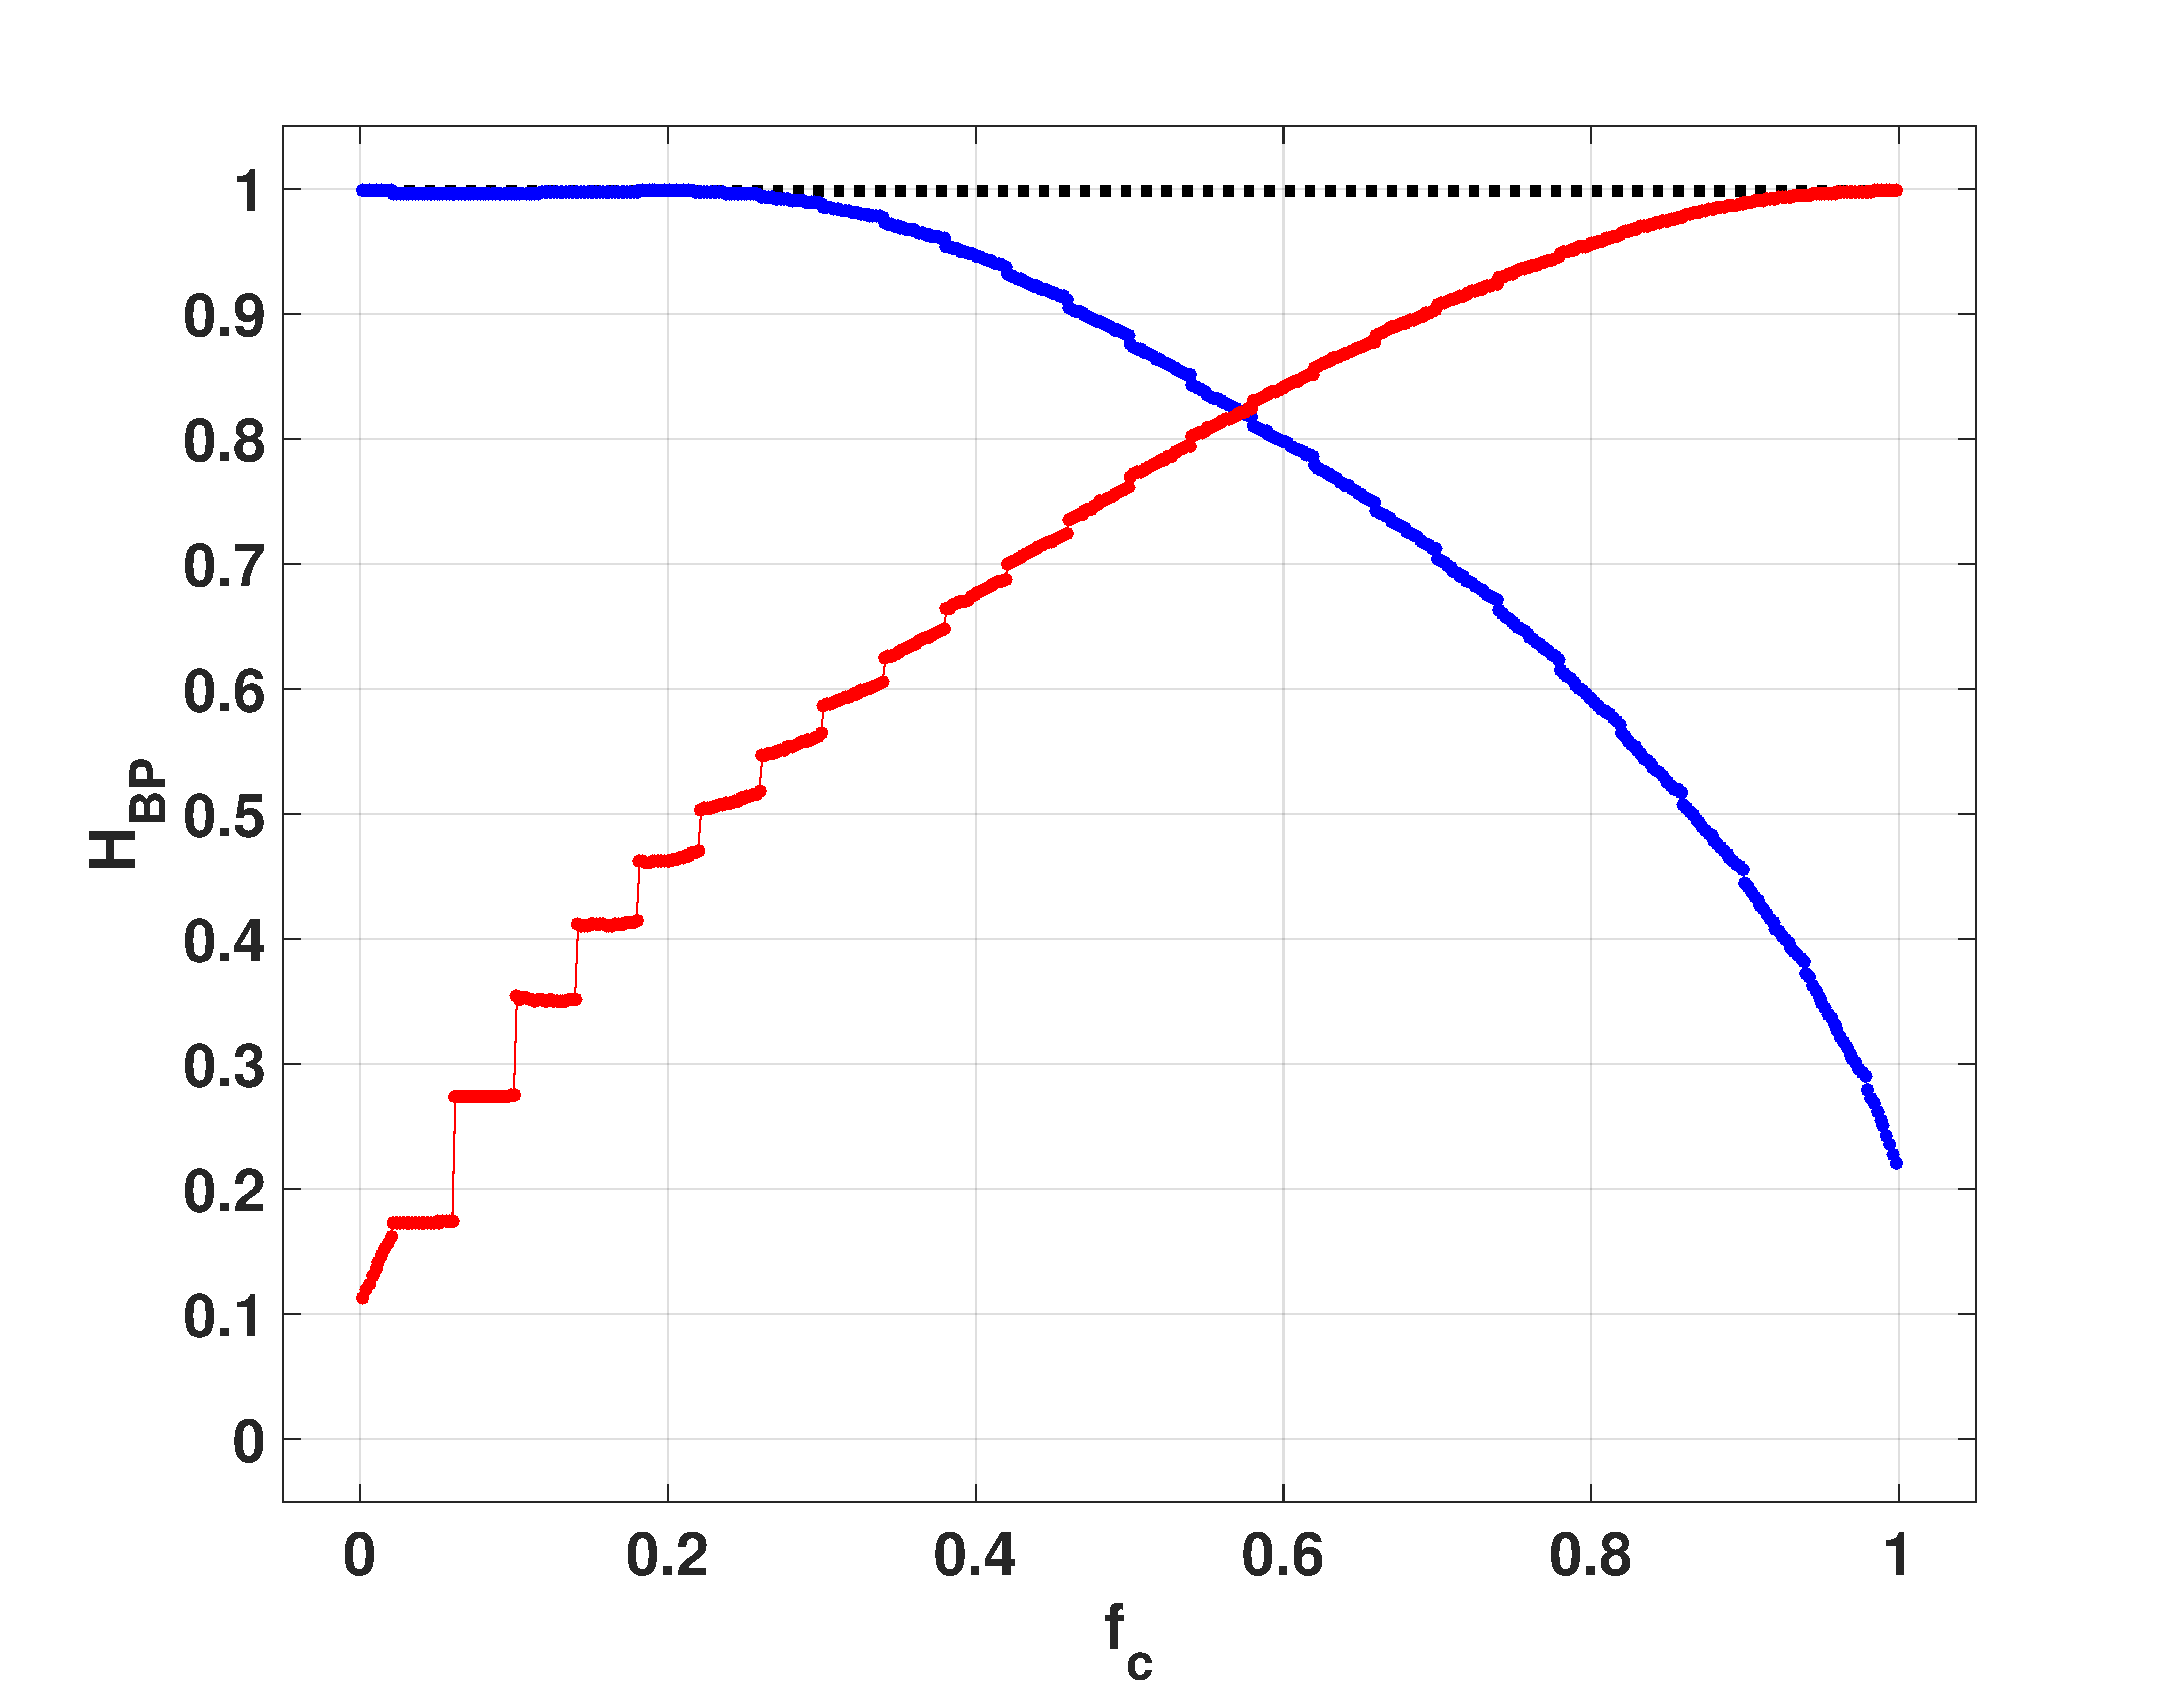
\includegraphics[width=\textwidth]{CuadradaRuidosa_Hbp}
        \caption{Entropía de patrones de orden normalizada}
        \label{subfig:CuadradaRuidosa_Hbp}
    \end{subfigure}
    ~ %add desired spacing between images, e. g. ~, \quad, \qquad, \hfill etc. 
    %(or a blank line to force the subfigure onto a new line)
    \begin{subfigure}[t]{0.32\textwidth}
        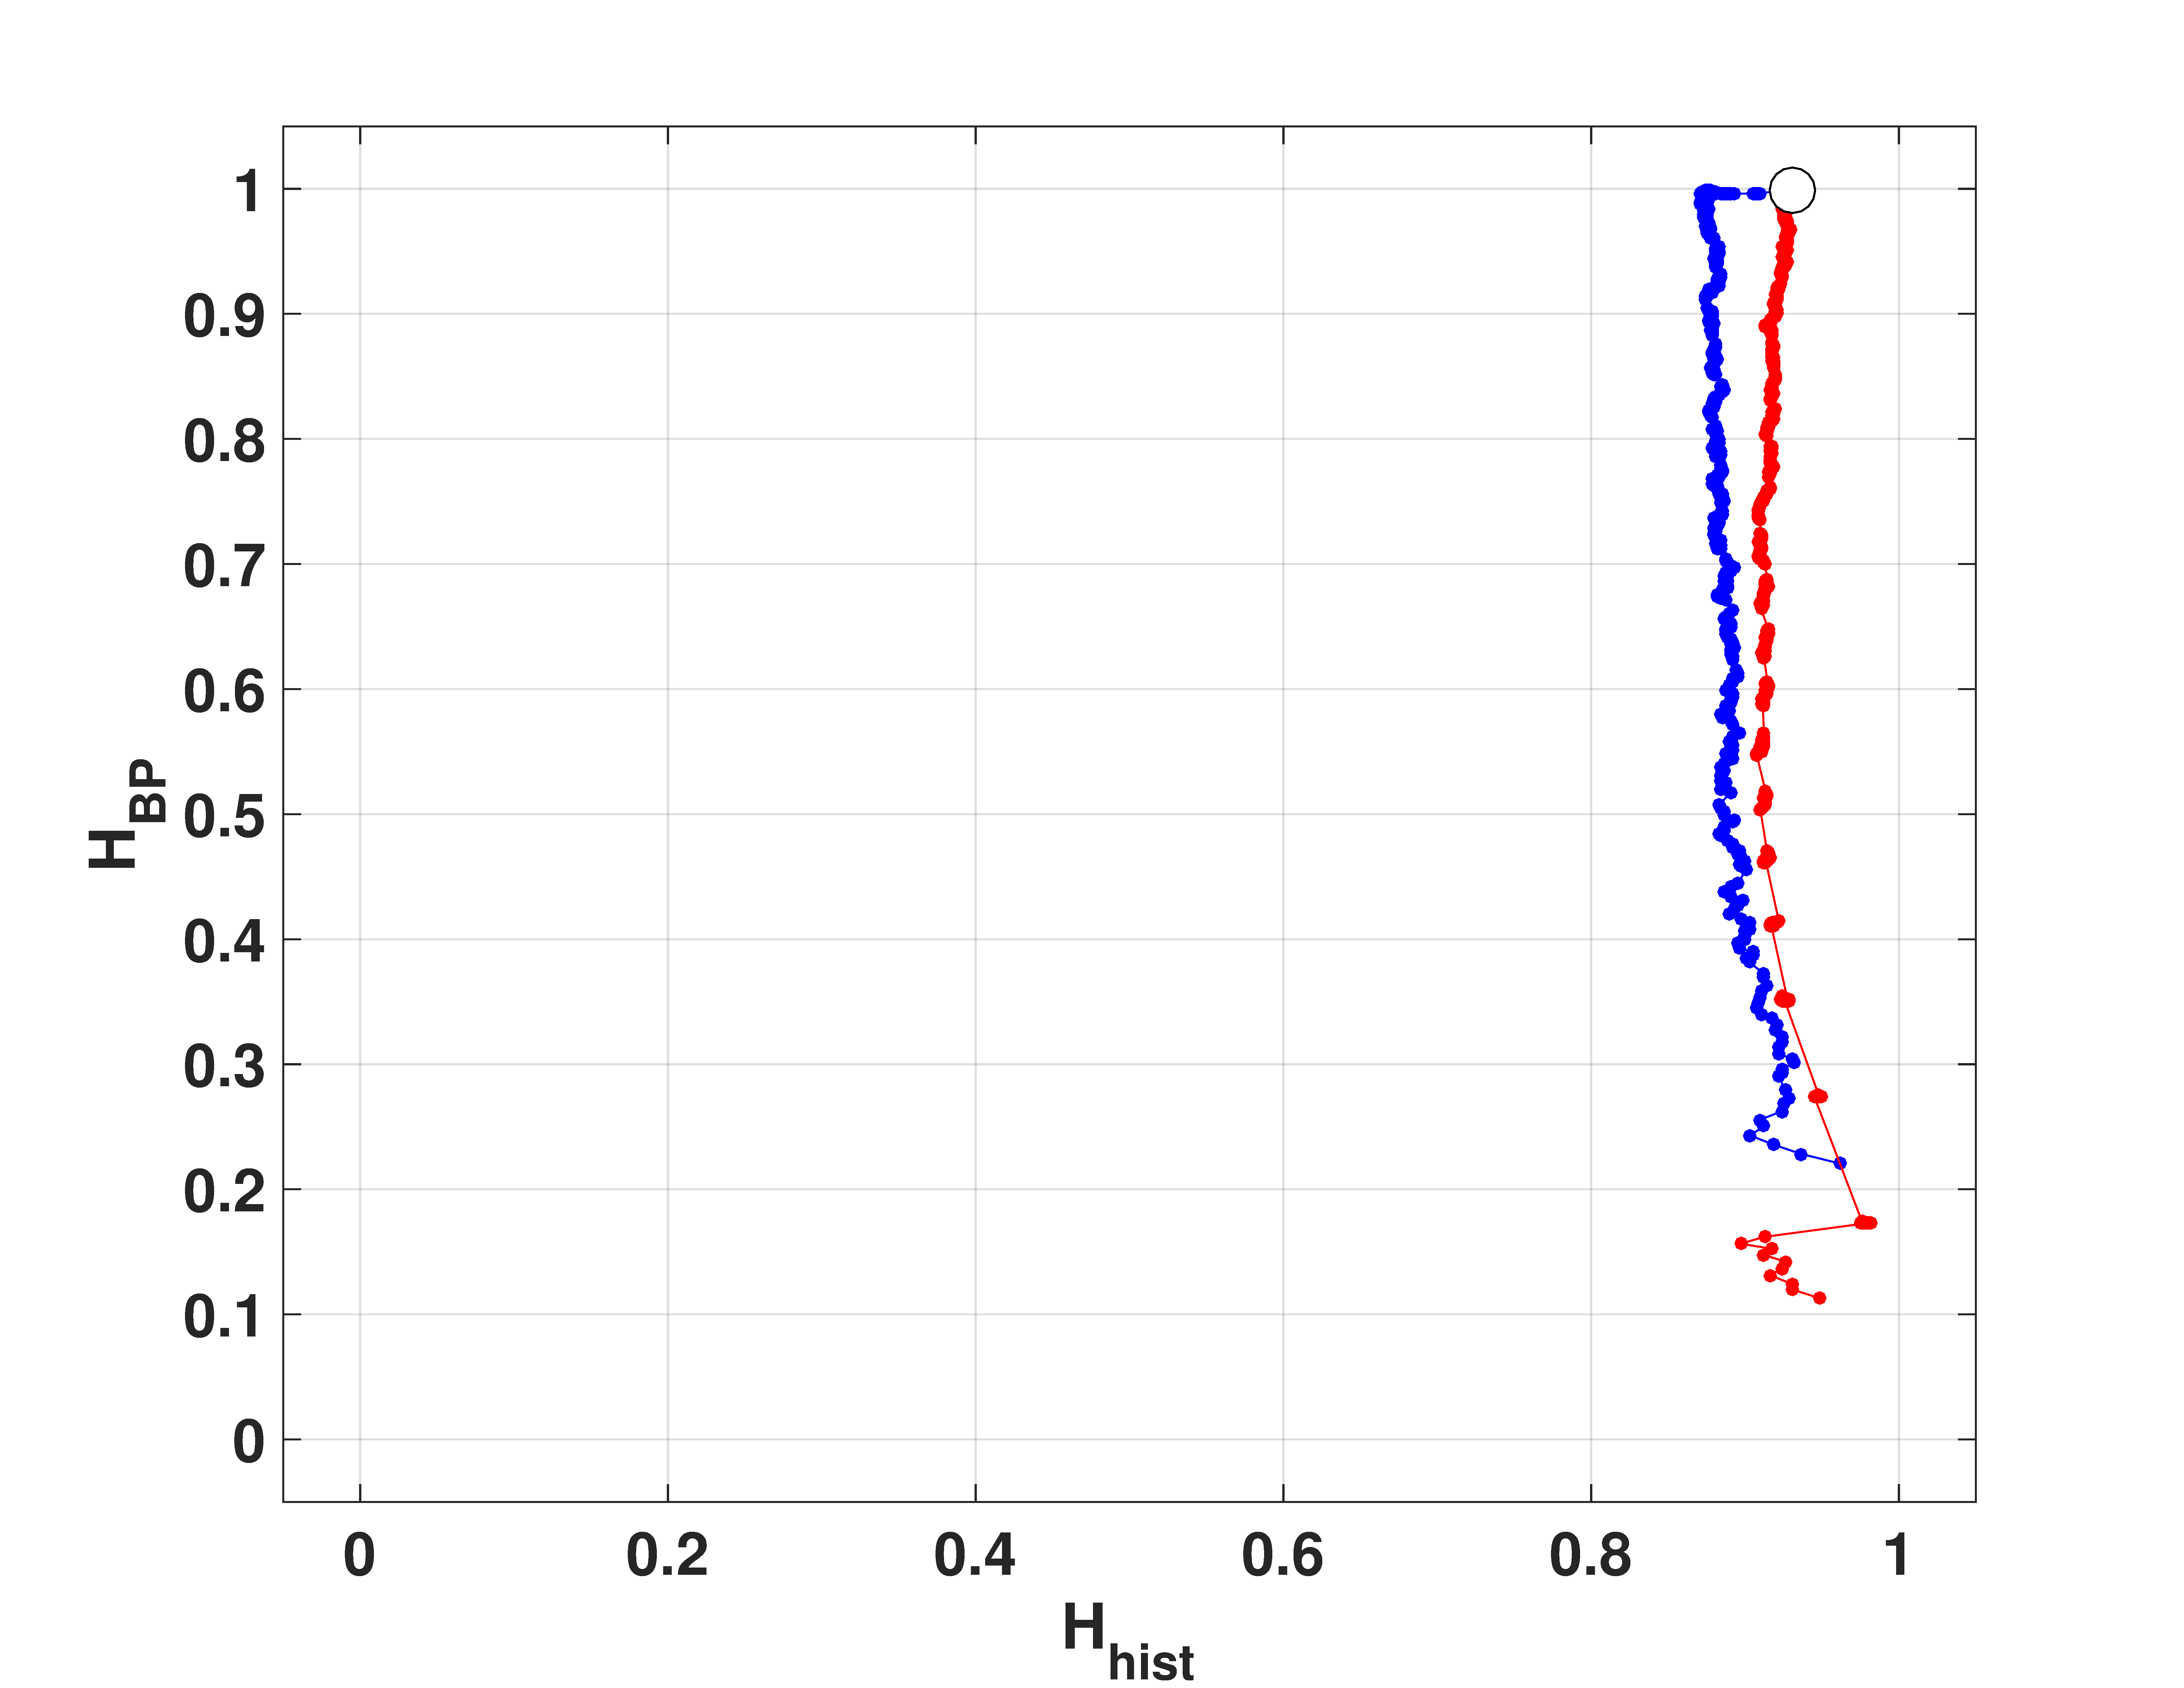
\includegraphics[width=\textwidth]{CuadradaRuidosa_Hbp_Hhist}
        \caption{Plano deoble entropía}
        \label{subfig:CuadradaRuidosa_HbpHhist}
    \end{subfigure}
    \caption{Cuantificadores calculados sobre la salida del filtro ideal cuando se ingresa con una cuadrada ruidosa.}\label{fig:CuadradaRuidosa}
\end{figure}

Para caracterizar el comportamiento de los cuantificadores frente a la amplitud de ruido, se generaron cuadradas contaminadas con AWGN de dos amplitudes y se filtraron para calcular cuantificadores.
En la figura \ref{fig:HCuadradaRuidosa_Sigma} se muestran ambos cuantificadores cuando se hace variar el ruido con valores de la desviación estándar $\sigma=[0~0,1~1]$.
Cuando comparamos las figuras \ref{subfig:HhistCuadradaRuidosa_Sigma_0}, \ref{subfig:HhistCuadradaRuidosa_Sigma_0p1} y \ref{subfig:HhistCuadradaRuidosa_Sigma_1} vemos un cambio significativo cuando pasamos de la señal limpia de \ref{subfig:HhistCuadradaRuidosa_Sigma_0} a la contaminada con bajos niveles de ruido de la \ref{subfig:HhistCuadradaRuidosa_Sigma_0p1}, sin embargo cuando pasamos del bajo nivel de ruido de \ref{subfig:HhistCuadradaRuidosa_Sigma_0p1} al de la figura \ref{subfig:HhistCuadradaRuidosa_Sigma_1} el cambio es mucho más sutil.
De modo similar, entre las figuras \ref{subfig:HbpCuadradaRuidosa_Sigma_0} y \ref{subfig:HbpCuadradaRuidosa_Sigma_0p1} hay muy poco parecido, mientras que las figuras \ref{subfig:HbpCuadradaRuidosa_Sigma_0p1} y \ref{subfig:HbpCuadradaRuidosa_Sigma_1} son bastante similares.
En este segundo caso es más evidente la diferencia cuando cambia el nivel de ruido, con bajos niveles puede verse el escalonado que aparece cada vez que una frecuencia es filtrada, mientras que cuando la amplitud de ruido es mayor este escalonado aparece solo en el pasabajos para las tres primeras frecuencias, que resultan ser las de mayor peso.
%
\begin{figure}[h]
    \centering
    \begin{subfigure}[t]{0.32\textwidth}
        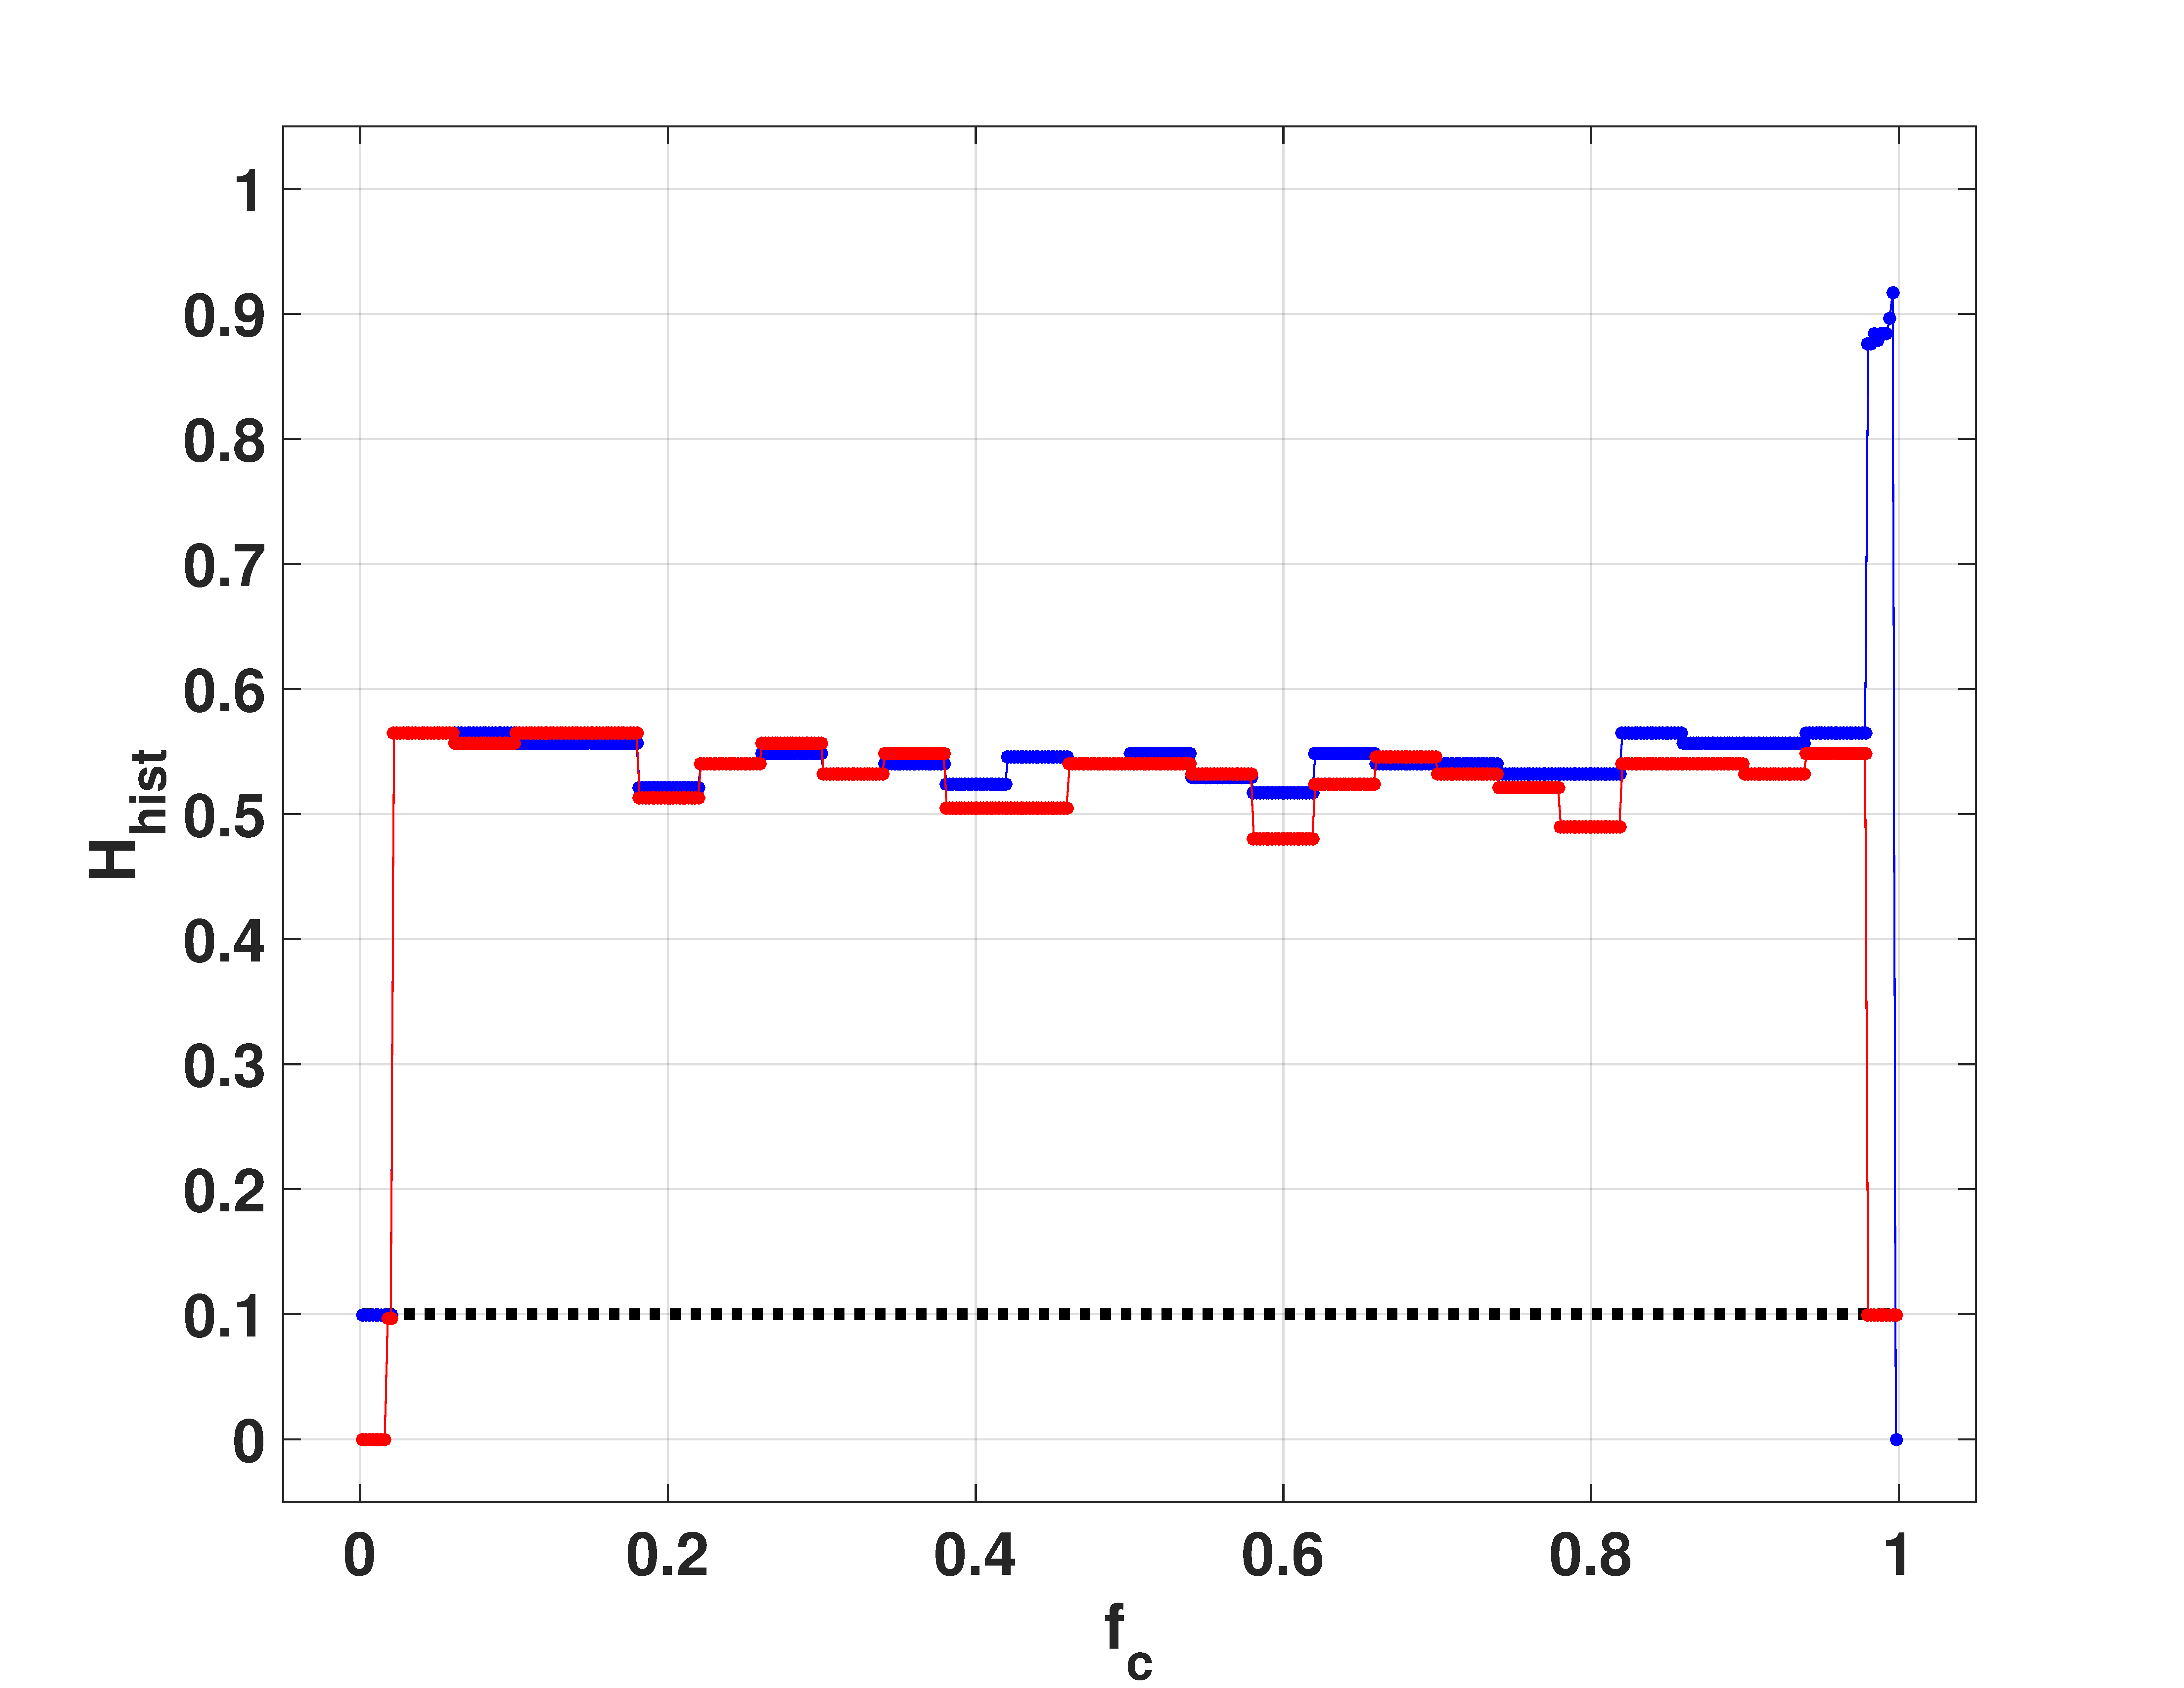
\includegraphics[width=\textwidth]{Cuadrada_Hhist}
        \caption{$H_{hist}$ con $\sigma=0$}
        \label{subfig:HhistCuadradaRuidosa_Sigma_0}
    \end{subfigure}
    ~ %add desired spacing between images, e. g. ~, \quad, \qquad, \hfill etc. 
      %(or a blank line to force the subfigure onto a new line)
    \begin{subfigure}[t]{0.32\textwidth}
        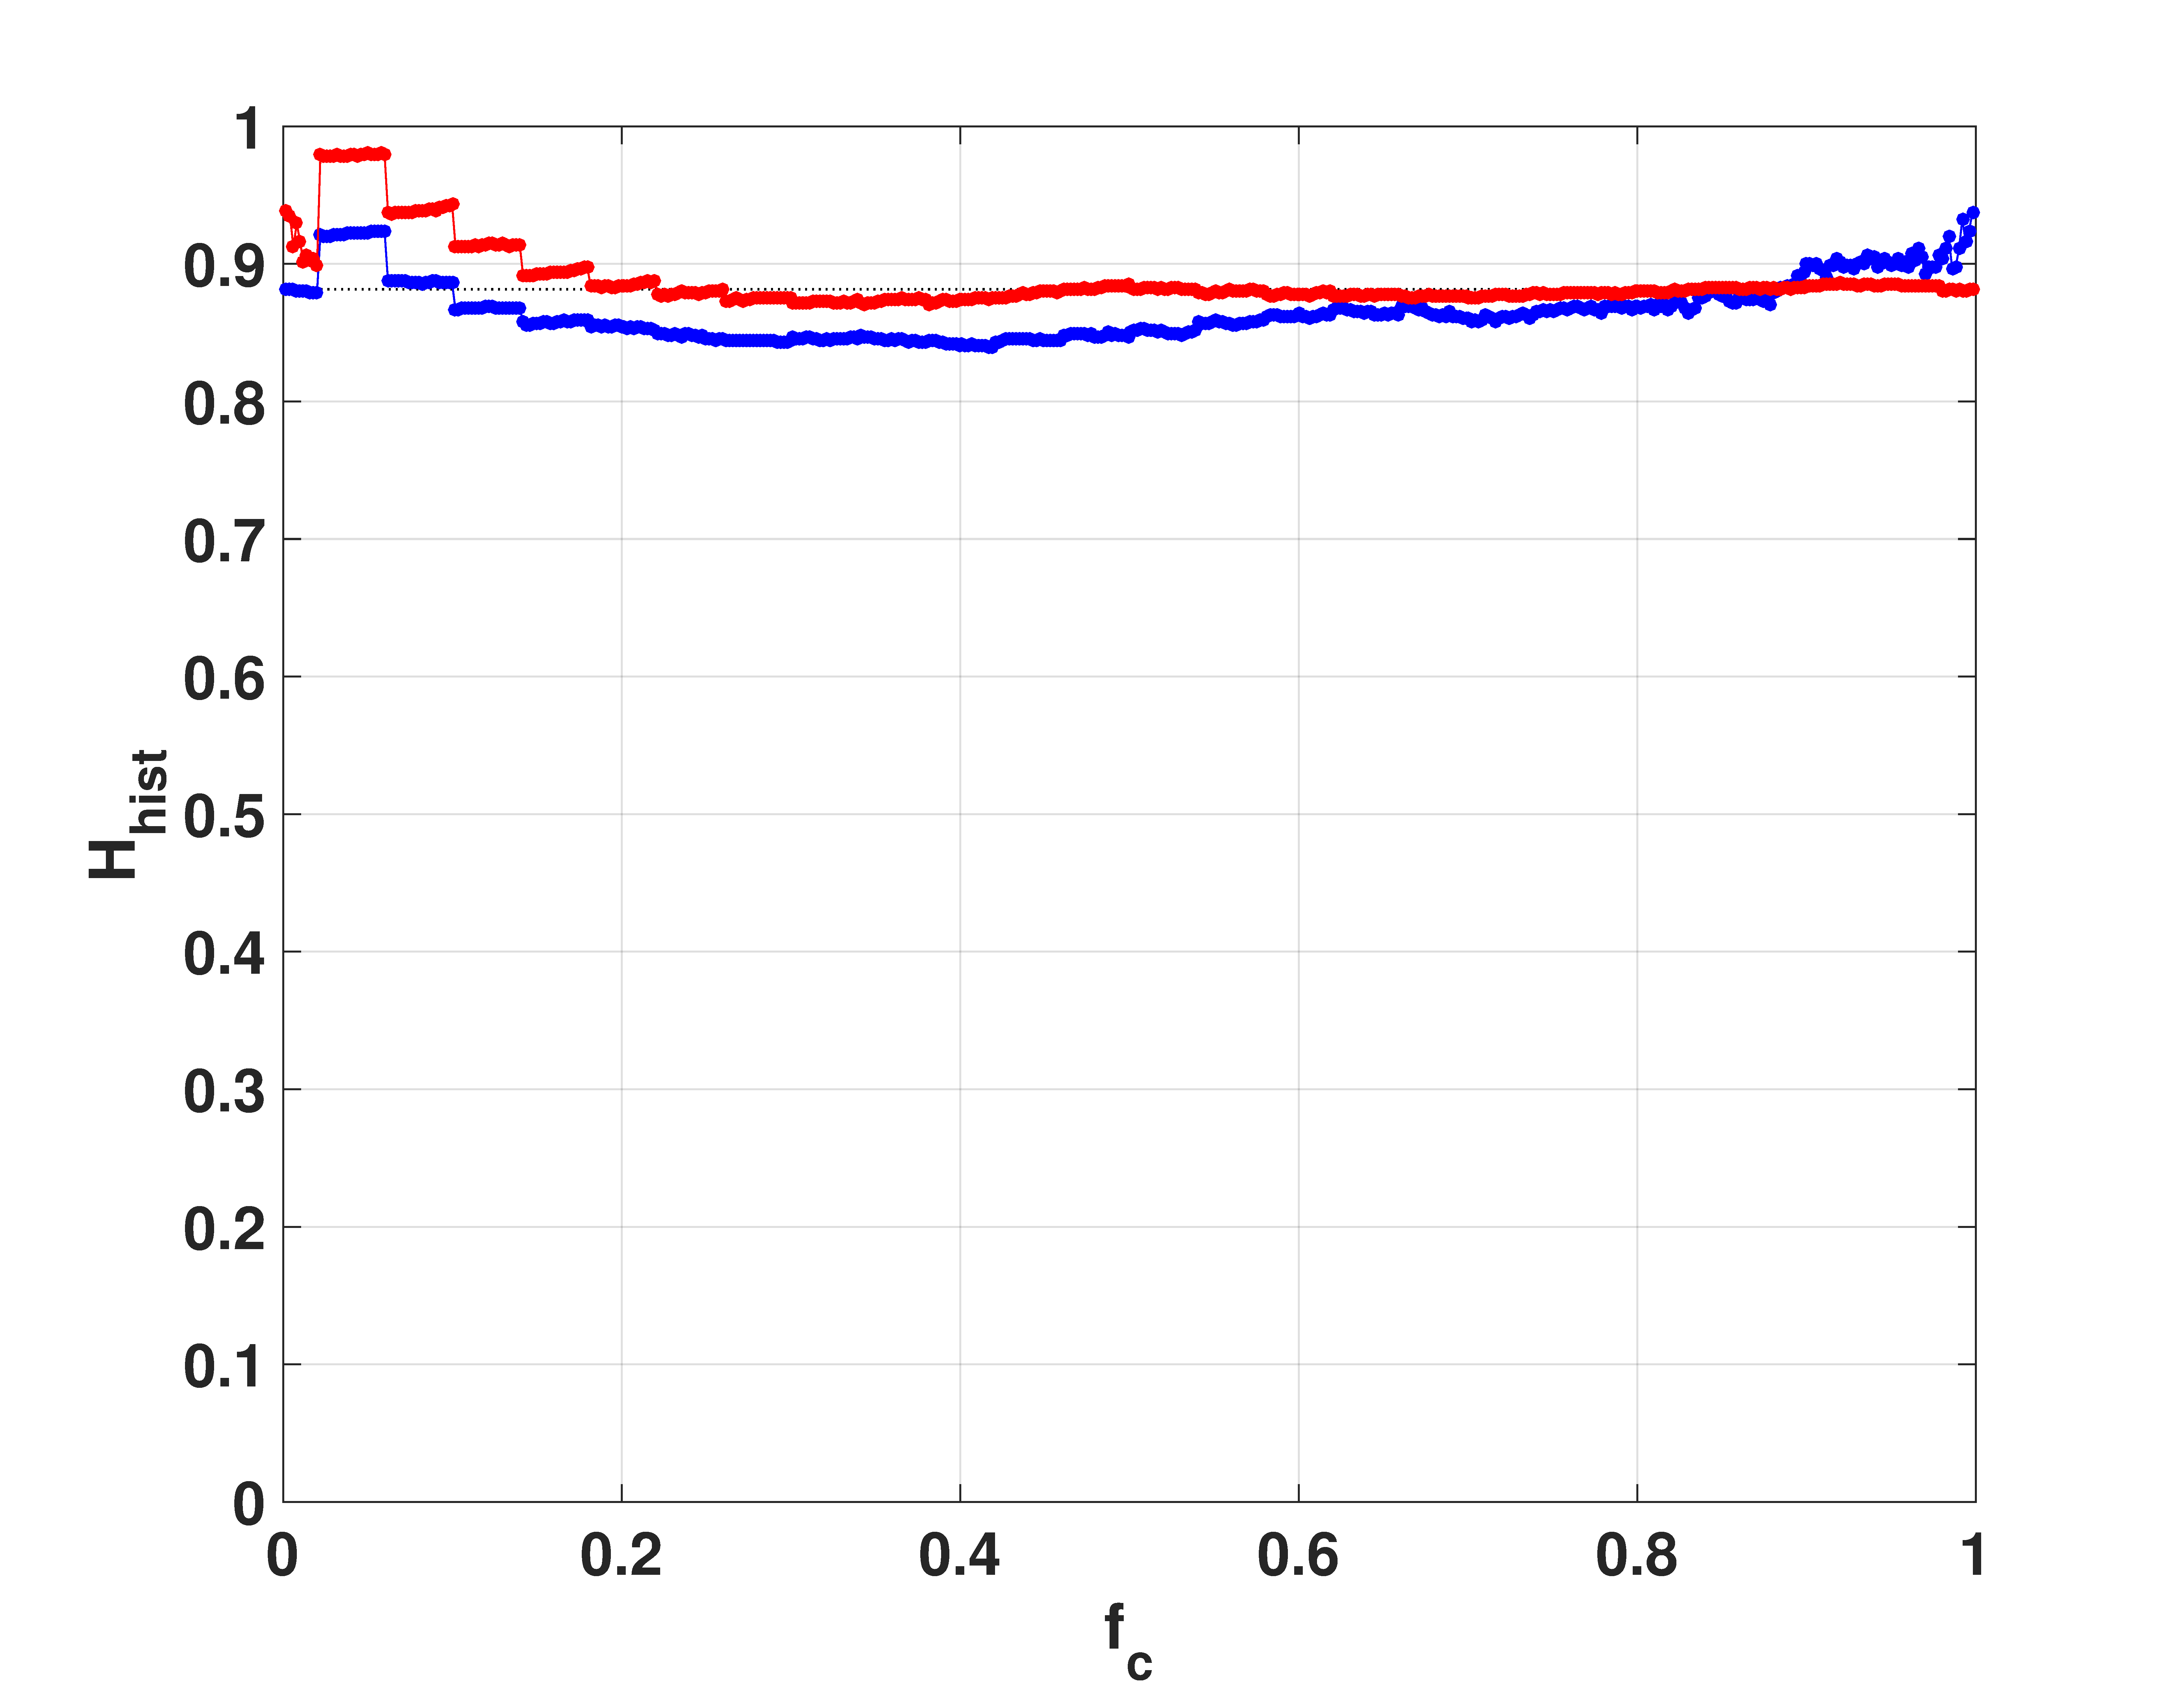
\includegraphics[width=\textwidth]{CuadradaRuidosa_Hhist_S0p1}
        \caption{$H_{hist}$ con $\sigma=0,1$}
        \label{subfig:HhistCuadradaRuidosa_Sigma_0p1}
    \end{subfigure}
    ~ %add desired spacing between images, e. g. ~, \quad, \qquad, \hfill etc. 
    %(or a blank line to force the subfigure onto a new line)
    \begin{subfigure}[t]{0.32\textwidth}
        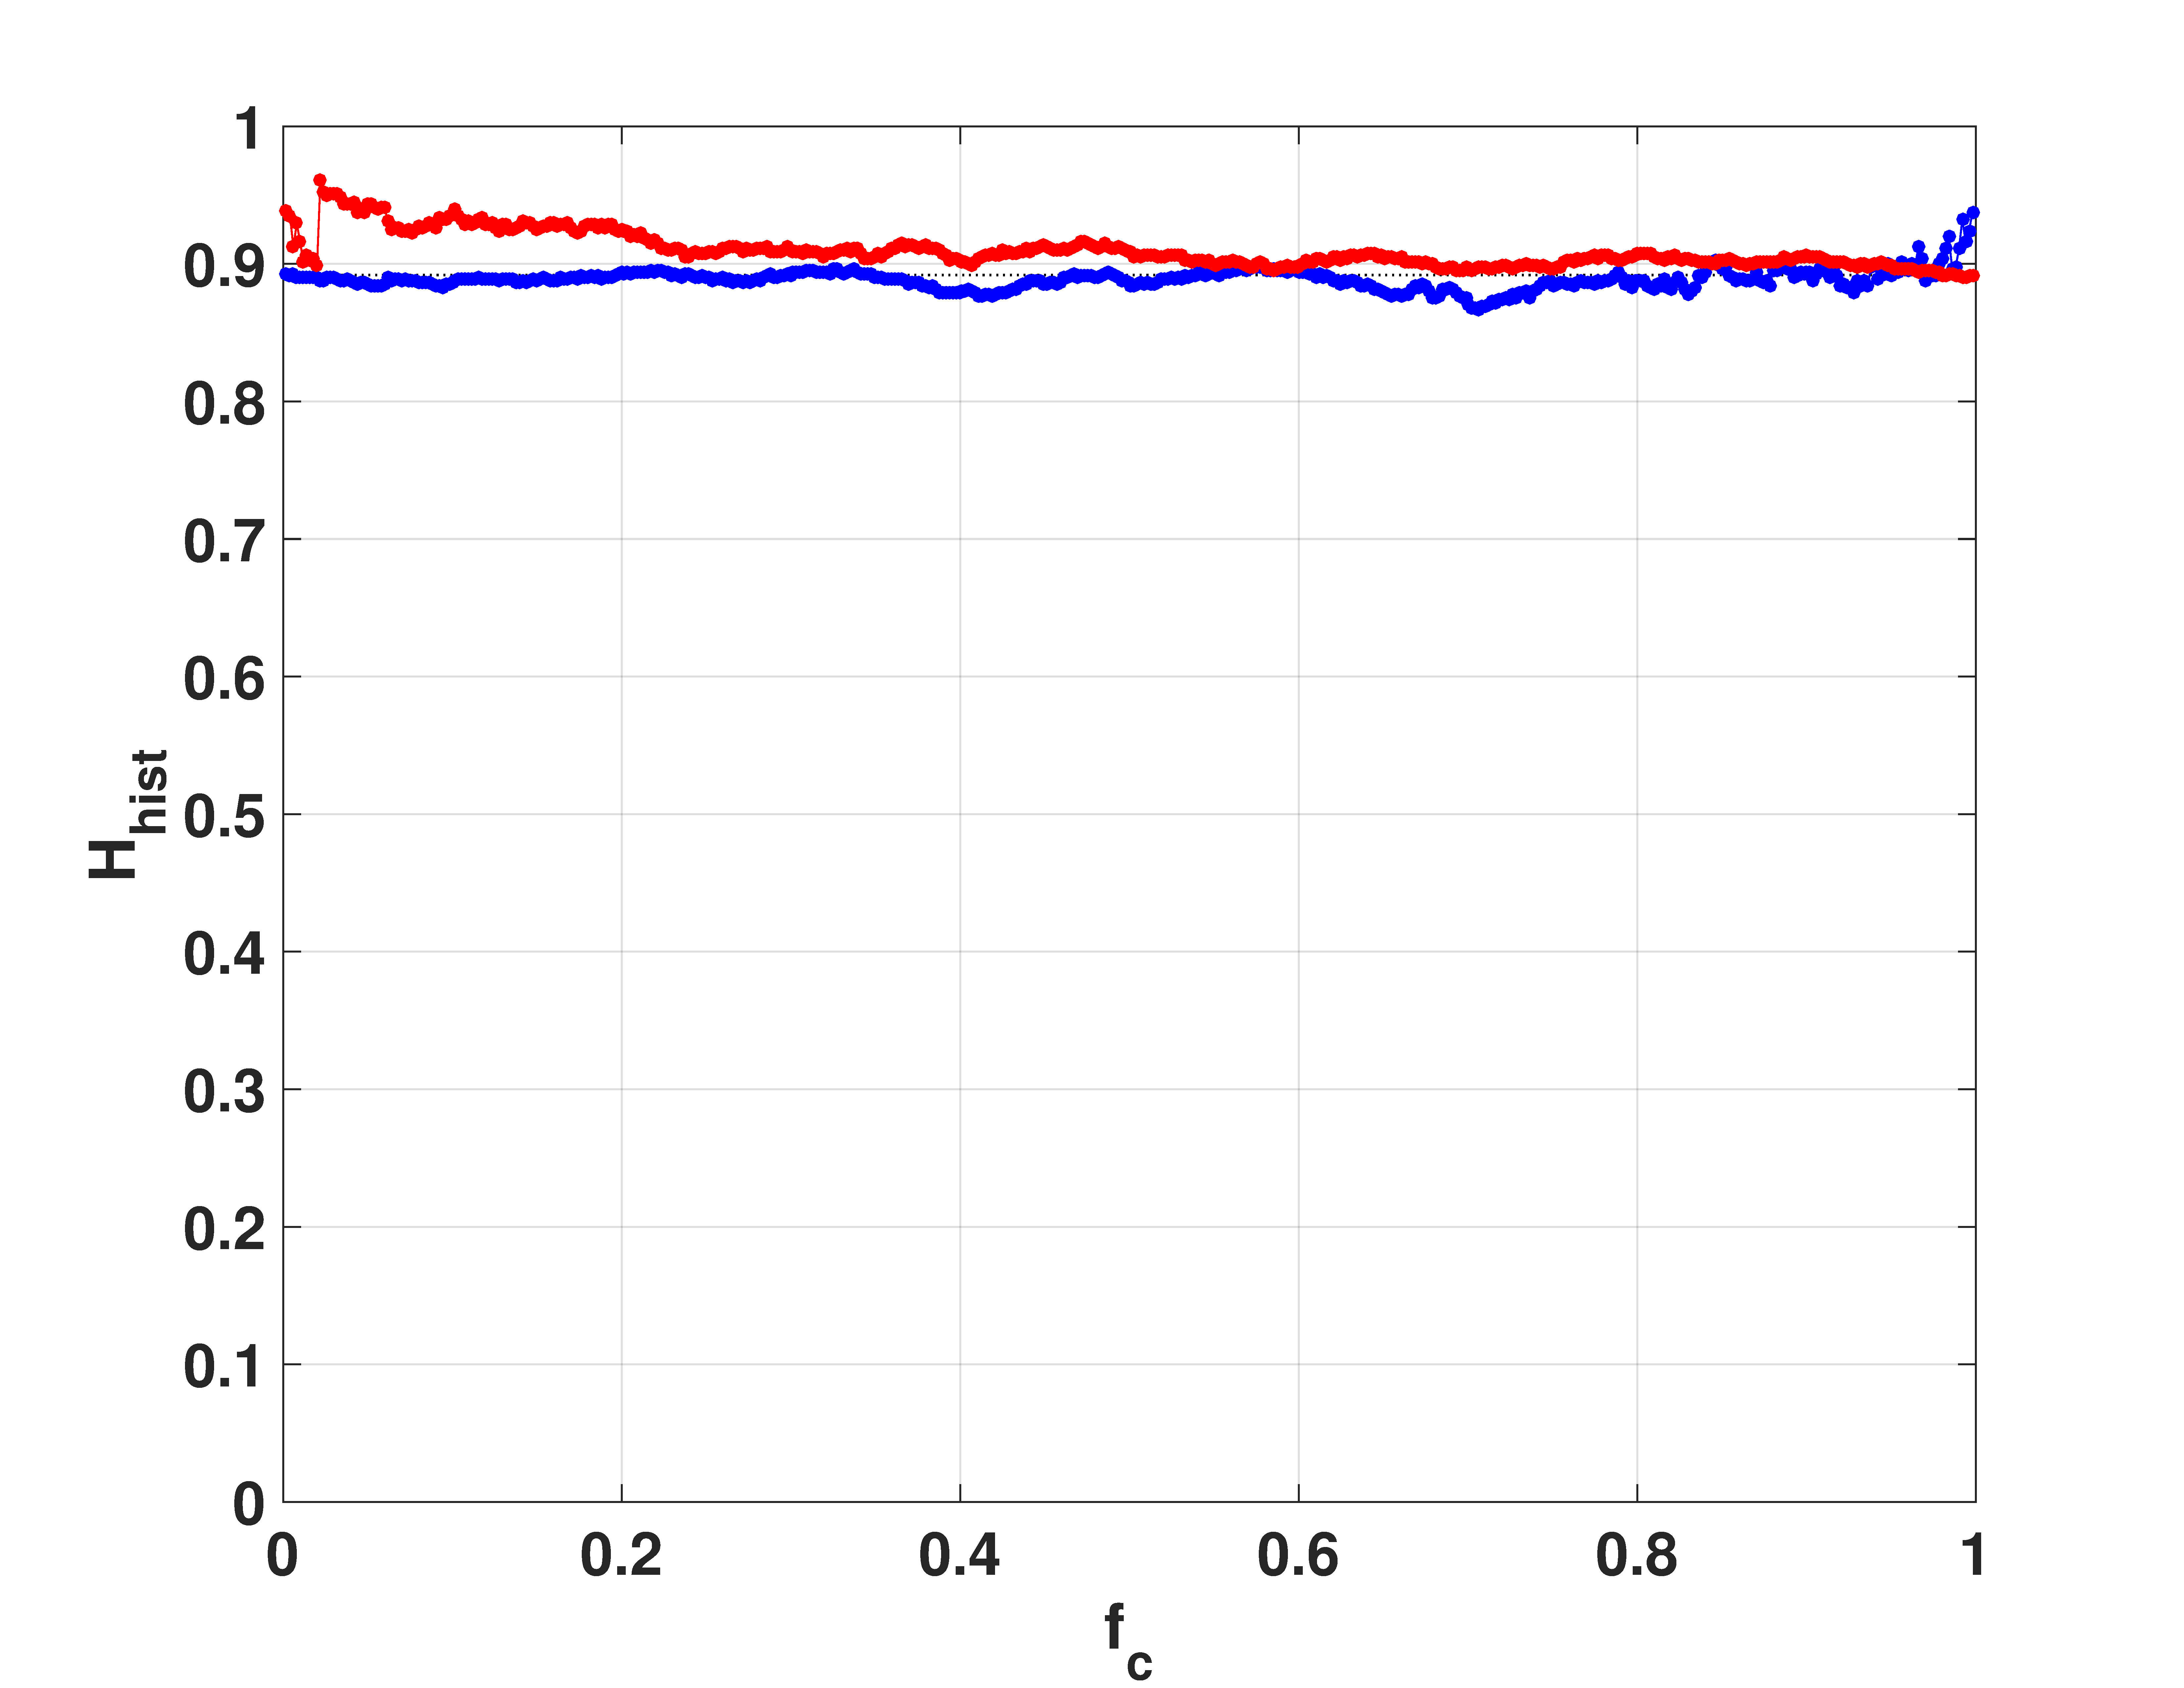
\includegraphics[width=\textwidth]{CuadradaRuidosa_Hhist_S1}
        \caption{$H_{hist}$ con $\sigma=1$}
        \label{subfig:HhistCuadradaRuidosa_Sigma_1}
    \end{subfigure}
    \begin{subfigure}[t]{0.32\textwidth}
        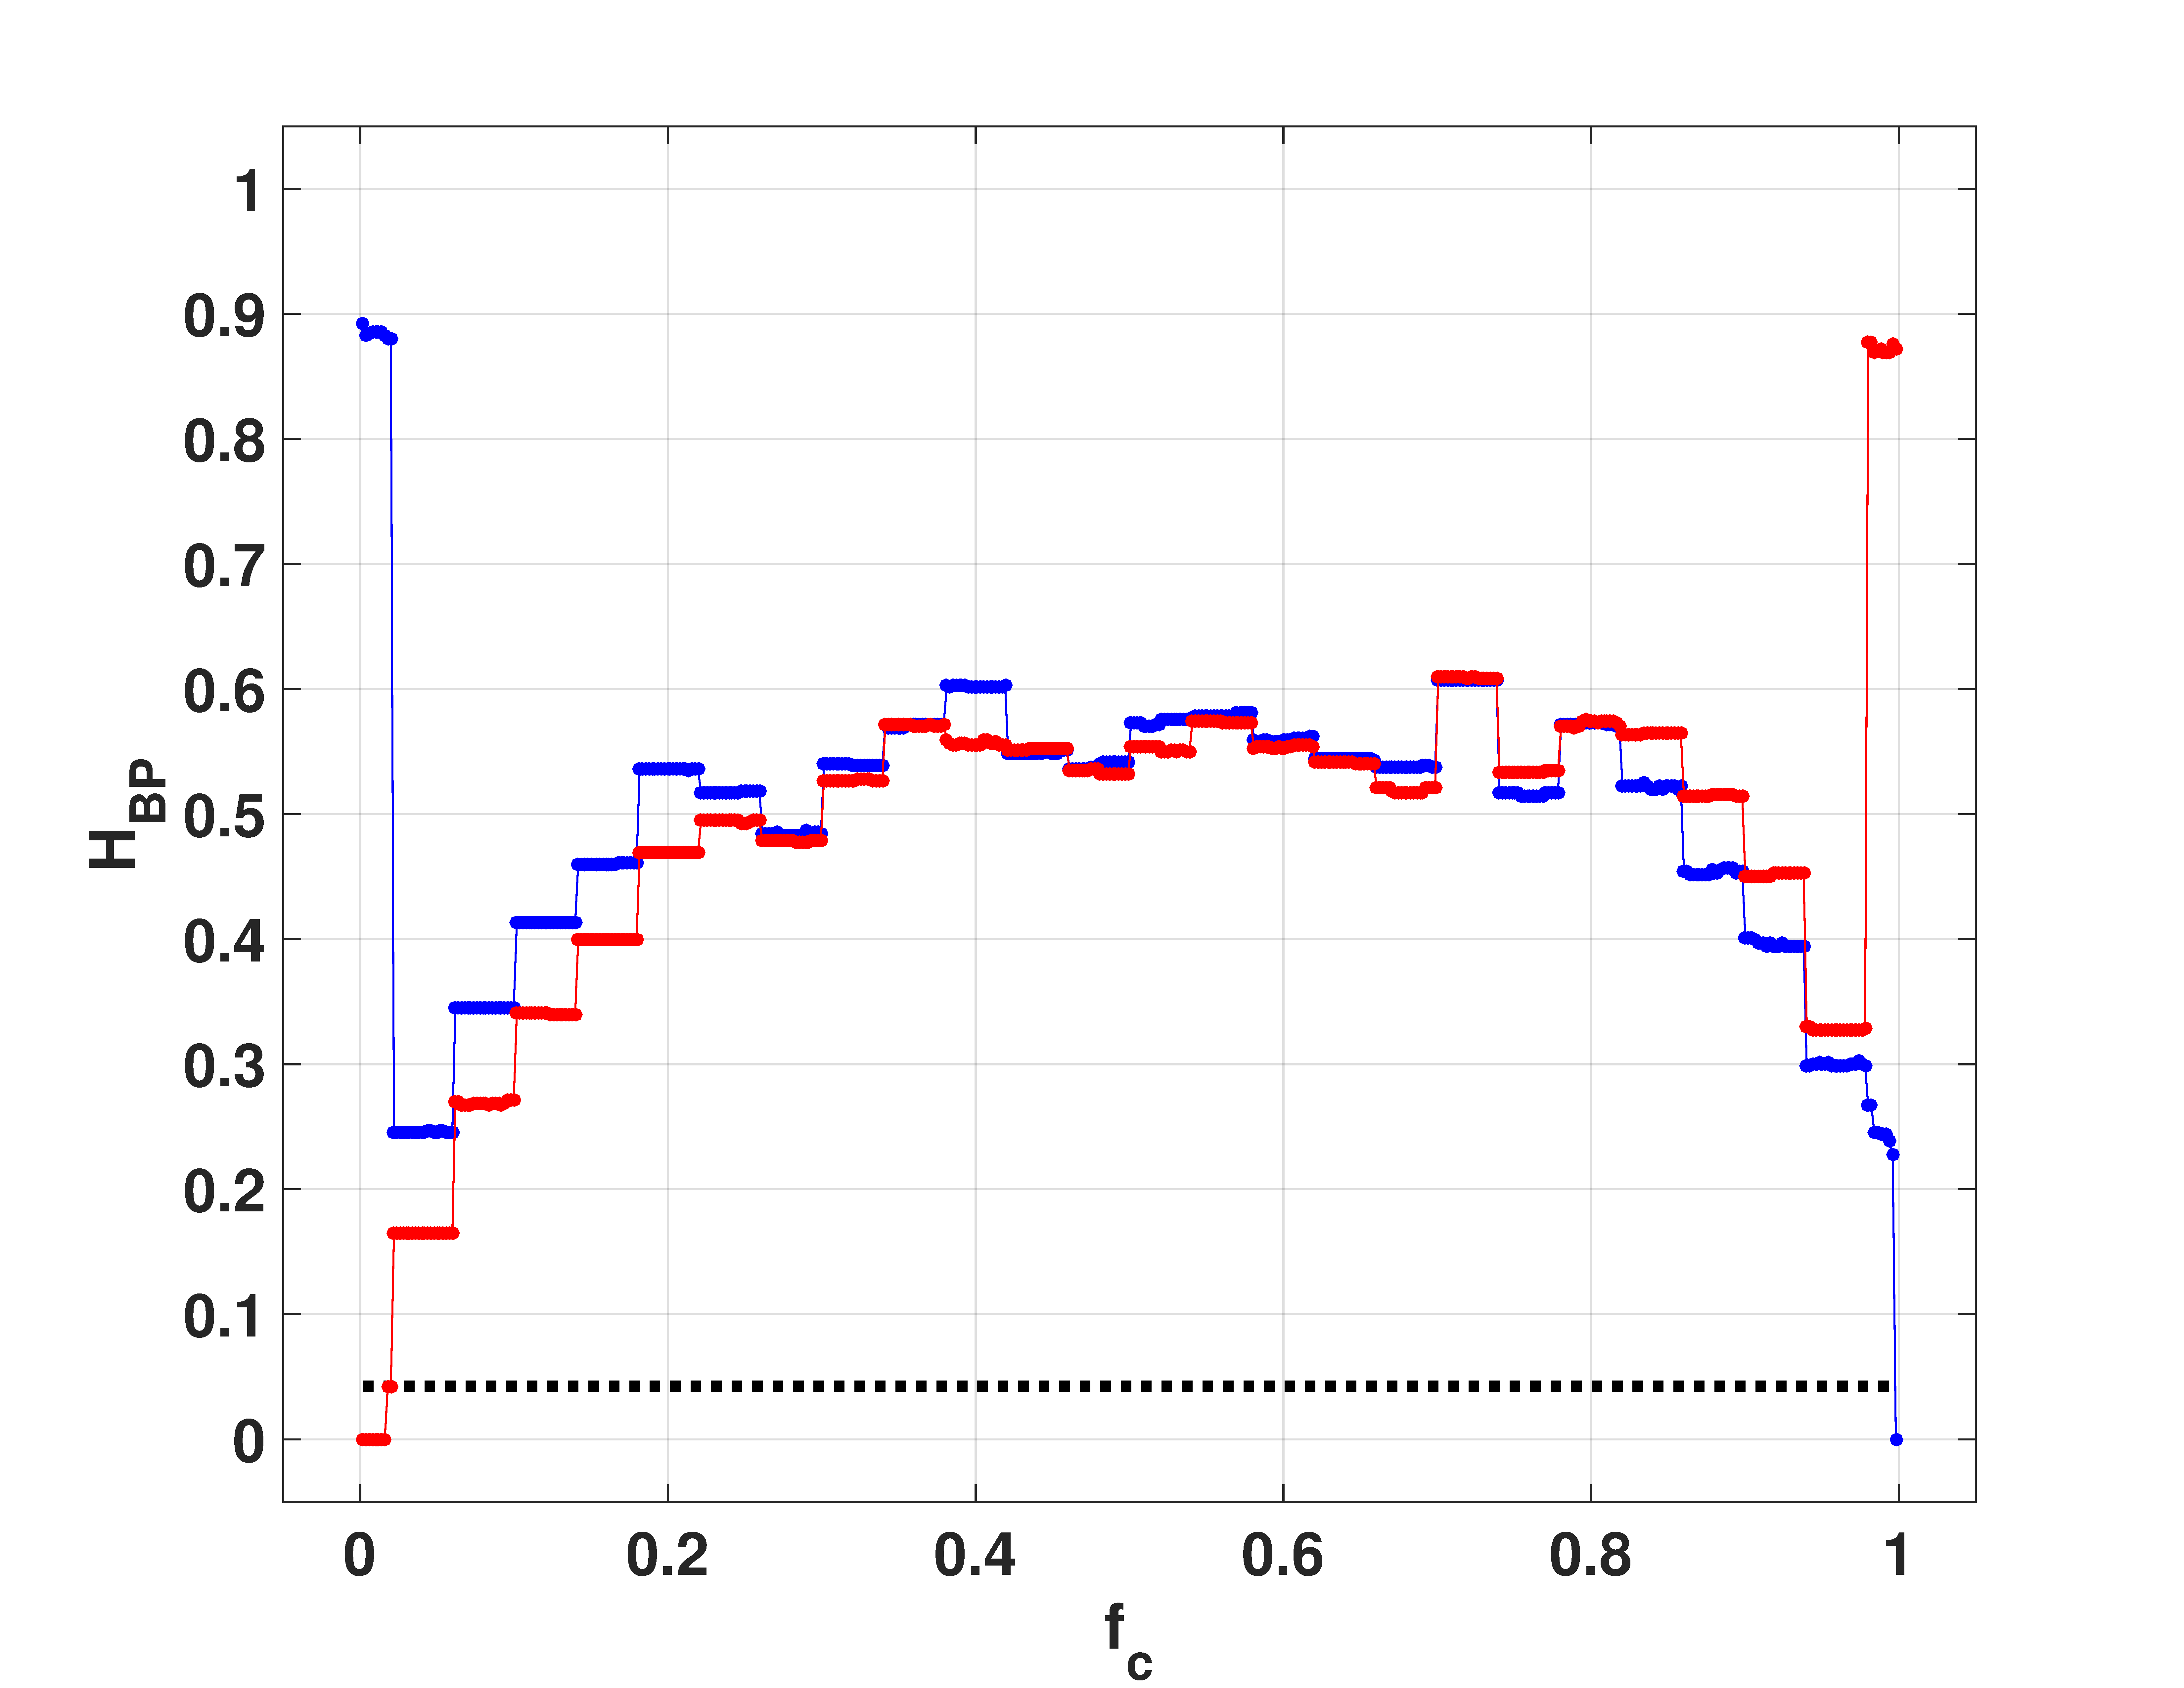
\includegraphics[width=\textwidth]{Cuadrada_Hbp}
        \caption{$H_{BP}$ con $\sigma=0$}
        \label{subfig:HbpCuadradaRuidosa_Sigma_0}
    \end{subfigure}
    ~ %add desired spacing between images, e. g. ~, \quad, \qquad, \hfill etc. 
      %(or a blank line to force the subfigure onto a new line)
    \begin{subfigure}[t]{0.32\textwidth}
        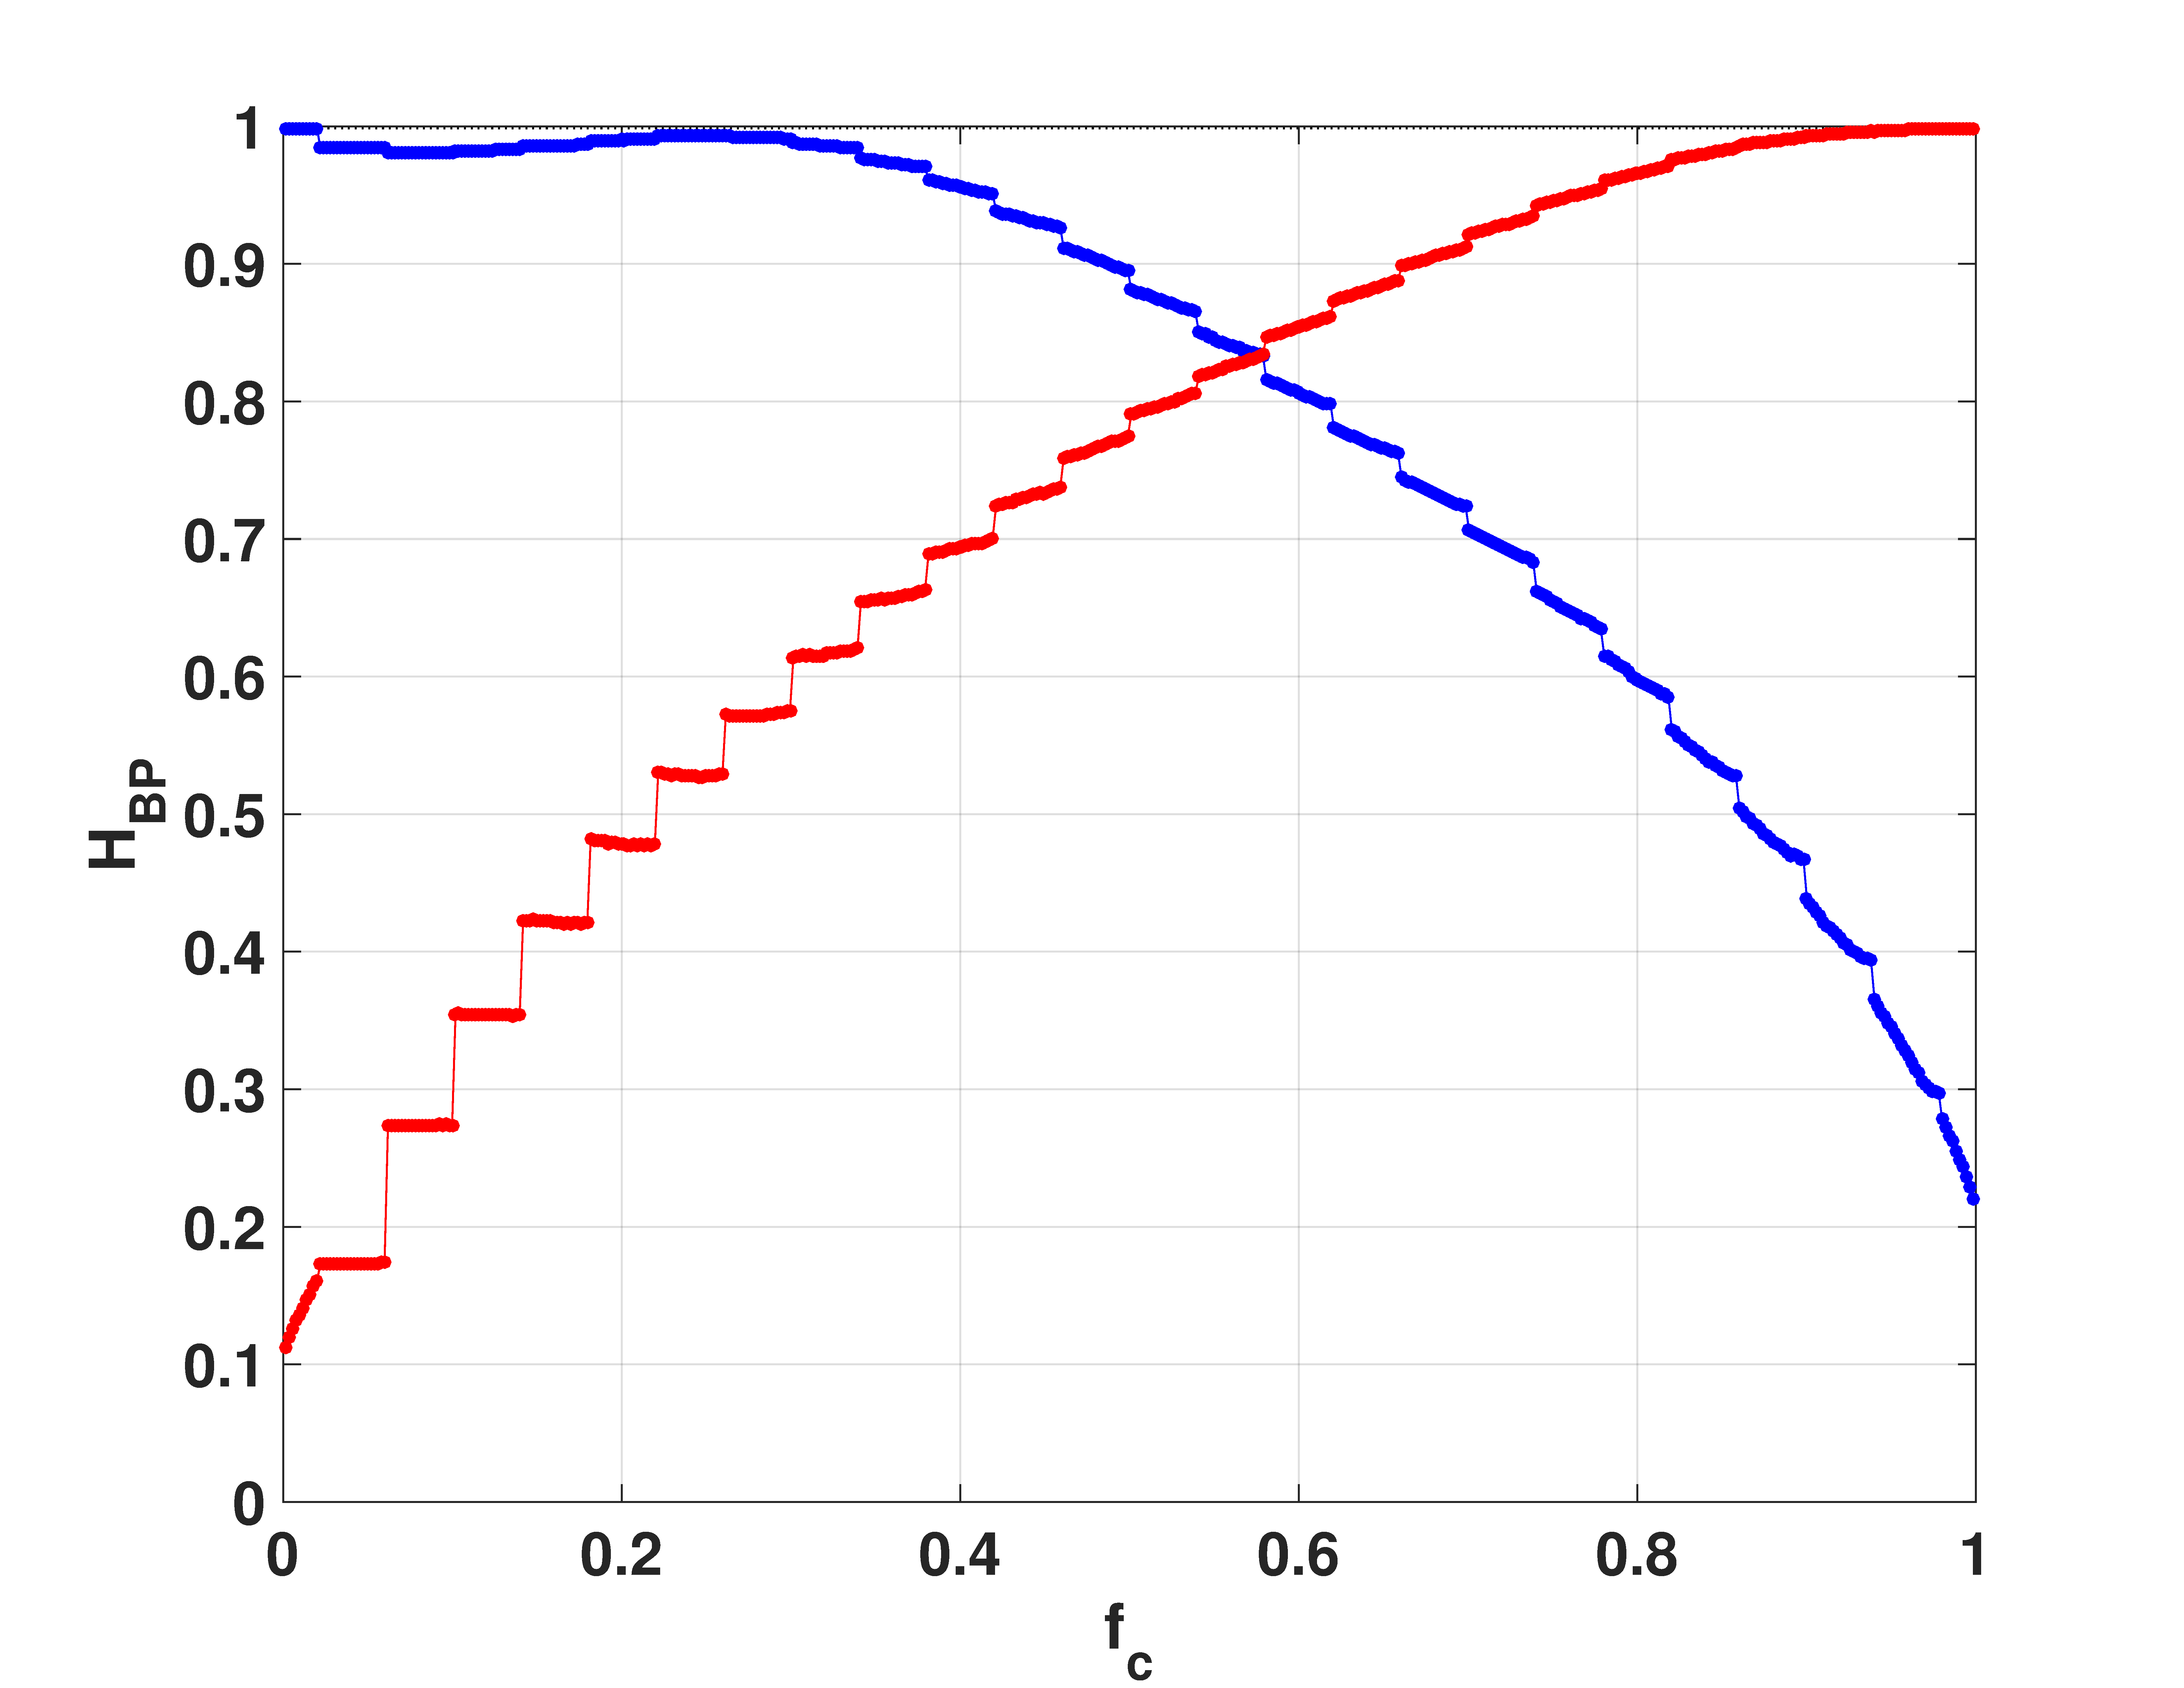
\includegraphics[width=\textwidth]{CuadradaRuidosa_Hbp_S0p1}
        \caption{$H_{BP}$ con $\sigma=0,1$}
        \label{subfig:HbpCuadradaRuidosa_Sigma_0p1}
    \end{subfigure}
    ~ %add desired spacing between images, e. g. ~, \quad, \qquad, \hfill etc. 
    %(or a blank line to force the subfigure onto a new line)
    \begin{subfigure}[t]{0.32\textwidth}
        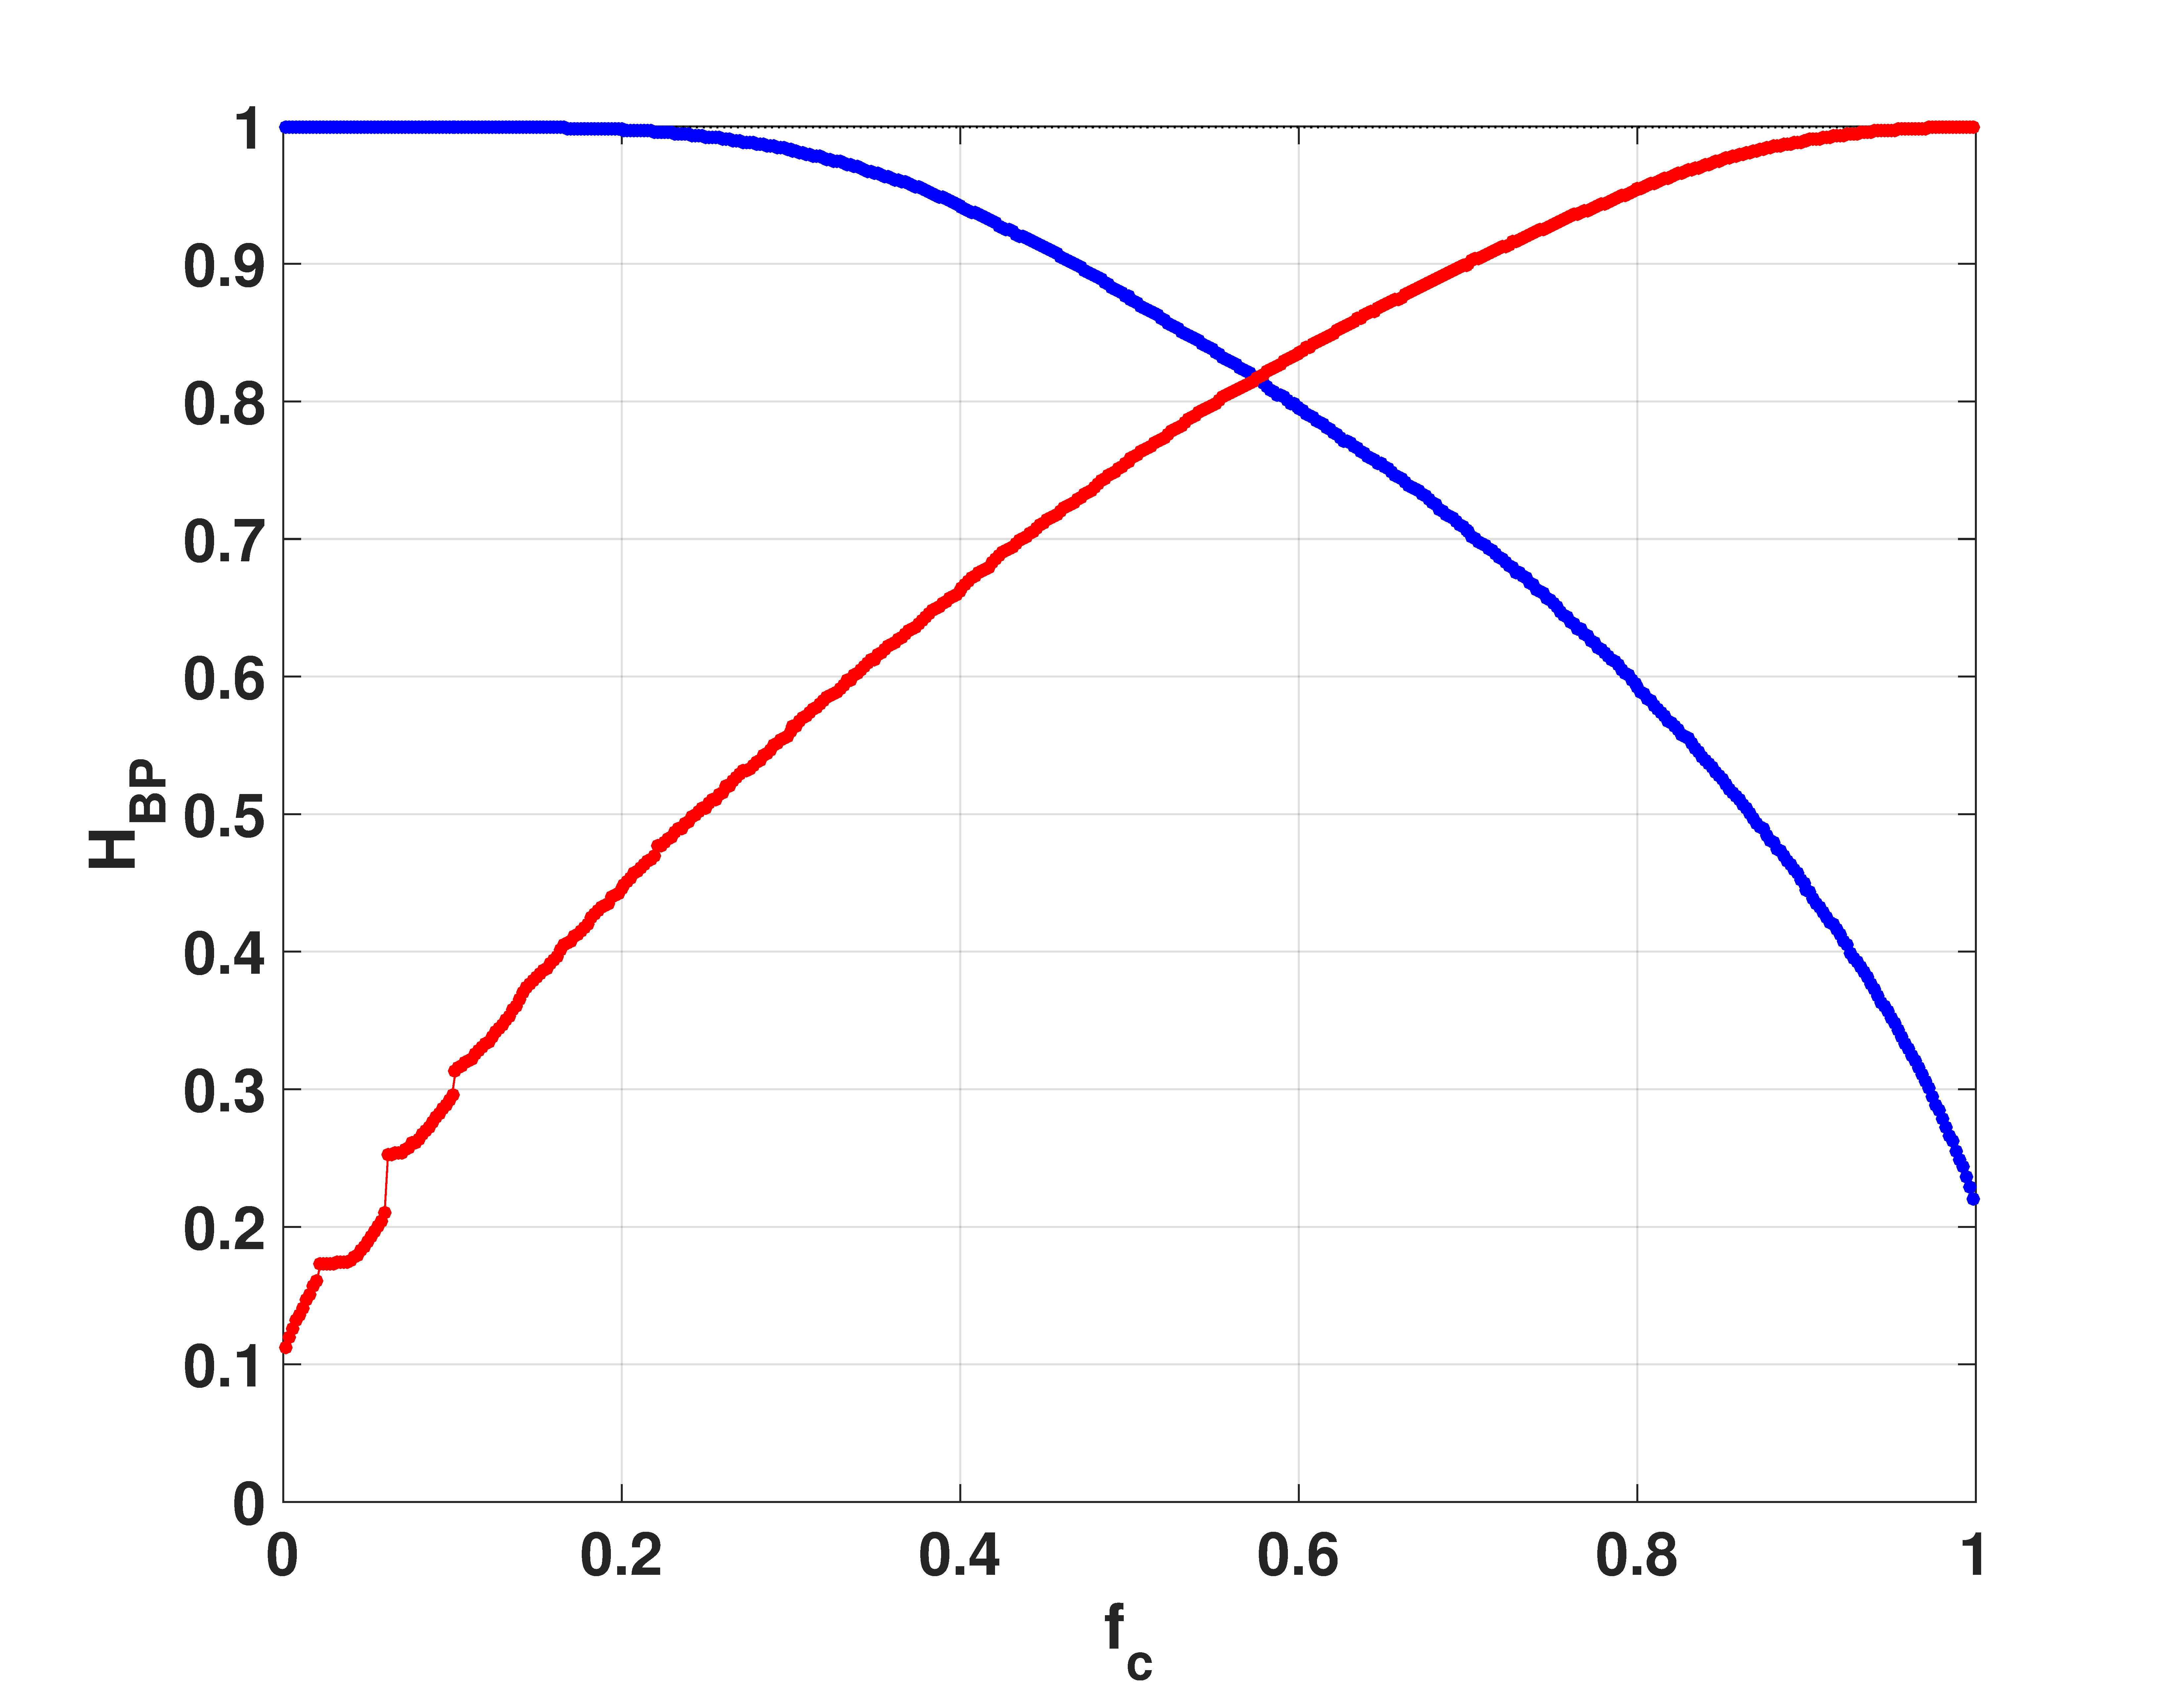
\includegraphics[width=\textwidth]{CuadradaRuidosa_Hbp_S1}
        \caption{$H_{BP}$ con $\sigma=1$}
        \label{subfig:HbpCuadradaRuidosa_Sigma_1}
    \end{subfigure}
    \caption{Cuantificadores calculados sobre la salida del filtro ideal cuando se ingresa con cuadradas contaminadas con AWGN de con amplitudes de ruido $\sigma=[0~0.1~1]$.}\label{fig:HCuadradaRuidosa_Sigma}
\end{figure}

\subsubsection{Discusión}
\label{sec:discusion}

Este trabajo fue necesario para explorar las fuentes de error en un medidor de entropías implementado en FPGA.

Para este primer análisis evaluamos que sucede aplicando un filtro abrupto, es por esto que elegimos para comparar un filtro elíptico y uno ideal. 
Las respuestas del filtro elíptico y del ideal fueron muy similares en el rango de frecuencias en los que el elíptico tiene un buen comportamiento, sin embargo cuando la frecuencia de corte del elíptico se acerca a los extremos (es decir cuando $f_c \to 0$ o $f_c \to 1$) la salida del filtro diverge.
El problema se debe a que el método numérico utilizado para calcular la salida del filtro diverge por la precisión finita utilizada.
Como no necesitamos volver a la frecuencia contínua nos quedamos con los resultados del ideal para hacer las pruebas, sin tener que procuparnos por el ripple que aparece en las bandas de paso y rechazo cuando pasamos al mundo analógico.

Cuando comparamos las respuestas de los cuantificadores con y sin ruido, vemos que las señales limpias tienen mesetas, es decir que se mantienen constantes hasta que el filtrado elimina la siguiente componente espectral.
Sin embargo, cuando son contaminadas con ruido los cuantificadores cambian para parecerse más a los resultados que arroja el ruido blanco gaussiano sin ninguna señal determinística.
En todos los casos se vio que estos cuantificadores son muy sensibles a la presencia de ruido, los que nos permite vincular a este hecho los errores en la medición.

También vimos que los valores cambian a medida que se filtra la señal sin contaminar, lo que agrega una segunda fuente de error dada por el ancho de banda finito del sistema.

Para continuar con este proyecto faltaría, por un lado caracterizar el sistema de medición en cuanto a su ancho de banda y su rechazo al ruido aditivo, y por otro lado probar con otros cuantificadores (como complejidad, desequilibrio, entropía diferencial, rate entropy, etc) o con variantes de los presentados aquí (Bandt \& Pompe pesada, amplitud promedio en el emmbedding, etc).